%&format

% The above line adds the format that can be compiled with the following command:
% pdflatex -ini -jobname="format" "&pdflatex" mylatexformat.ltx """Phd-Thesis-Format.tex"""

\endofdump

%-------------------------------------------------------------------------------
% Configuration
%-------------------------------------------------------------------------------

% Include all chapters/sections so the references are present
% \includeonly{chapters/objects}

\newif\ifIMAGES
\IMAGEStrue

%-------------------------------------------------------------------------------
% Includes changing over time
%-------------------------------------------------------------------------------
% -----------------------------------------------------------------------
% Image helper functions

\newcommand{\newImage}[1]{
    \ifIMAGES
        \centering
        \IfFileExists{#1}{\includegraphics{#1}}{\includegraphics{figures/general/scorpion.jpg}}
    \else
    \fi
}
\newcommand{\newImageResize}[1]{
    \ifIMAGES
        \centering
        \IfFileExists{#1}{
            \resizebox{\textwidth}{!}{
                \includegraphics{#1}
            }
        }
        {
            \includegraphics{figures/general/scorpion.jpg}
        }
    \else
    \fi
}
\newcommand{\newImageResizeCustom}[2]{
    \ifIMAGES
        \centering
        \IfFileExists{#1}{
            \resizebox{#2\textwidth}{!}{
                \includegraphics{#1}
            }
        }
        {
            \includegraphics{figures/general/scorpion.jpg}
        }
    \else
    \fi
}
\newcommand{\newImageResizeHalf}[1]{
    \ifIMAGES
        \centering
        \IfFileExists{#1}{
            \resizebox{0.48\textwidth}{!}{
                \includegraphics{#1}
            }
        }
        {
            \includegraphics{figures/general/scorpion.jpg}
        }
    \else
    \fi
}
\newcommand{\newImageScale}[2]{
    \ifIMAGES
        \centering
        \IfFileExists{#1}{\includegraphics[scale=#2]{#1}}{\includegraphics{figures/general/scorpion.jpg}}
    \else
    \fi
}
\newcommand{\newImageScaleRot}[2]{
    \ifIMAGES
        \centering
        \IfFileExists{#1}{\includegraphics[scale=#2,angle=-90]{#1}}{\includegraphics{figures/general/scorpion.jpg}}
    \else
    \fi
}


% -----------------------------------------------------------------------
% Short cuts

\newcommand{\myc}[1]{Ref.~\cite{#1}}

\newcommand{\HWW}{$H\rightarrow WW^*$}
\newcommand{\HWWdet}{\ensuremath{H\,{\rightarrow}\,W^{\pm}W^{\mp^*}\,{\rightarrow}\,\ell^-\bar{\nu} \ell^+\nu}\hspace{0.07em}}
\def\myurl{\hfil\penalty 100 \hfilneg \hbox}
\newcommand{\HWWhalfdet}{\ensuremath{H\,{\rightarrow}\,$~$WW^*\,{\rightarrow}\,$~$\ell\nu\ell\nu}\xspace}
\newcommand*{\ZeroJet}{\ensuremath{N_\text{jet}{=}\,0}\xspace}
\newcommand*{\OneJet}{\ensuremath{N_\text{jet}{=}\,1}\xspace}
\newcommand{\Ztautau}{\mbox{$Z/\gamma^*\,{\rightarrow}\,\tau\tau$}\,}
\newcommand{\Nbjet}{\ensuremath{N_{\text{$b$-jet}}}}
\newcommand{\Njet}{\ensuremath{N_{\text{jet}}}}
\newcommand{\Ntrkjet}{\ensuremath{N_{\text{jet}}^{\text{trk jet}}}}
%\newcommand{\Nbjetsub}{\ensuremath{N_{\text{$b$-jet}}}}
\newcommand{\nbJet}{\ensuremath{N_{\text{$b$-jet}}}}
\newcommand{\nbtrkjet}{\ensuremath{N_{\text{$b$-jet}}^{\text{track}}}}
\newcommand{\nbcalojet}{\ensuremath{N_{\text{$b$-jet}}^{\text{calo}}}}
\newcommand{\nbjet}{\ensuremath{N_{\text{$b$-jet}}}}
\newcommand*{\Zpoiss}{\ensuremath{Z_{\text{exp}}^{\text{Poiss}}}}
\newcommand{\Nbjetsub}{\ensuremath{N_{\text{$b$-jet}}^{\pT\,{>}\,20\,\GeV}}}
\newcommand{\Nbjetnom}{\ensuremath{N_{\text{$b$-jet}}^{\pT\,{>}\,30\,\GeV}}}
\newcommand{\Nbjetbetween}{\ensuremath{N_{\text{$b$-jet}}^{20\,\GeV{<}\,\pT\,{<}\,30\,\GeV}}}

\newcommand*{\bcaloveto}{\ensuremath{N^{\pT>20\,\GeV}_{\text{$b$-calo-jet}} = 0}}
\newcommand*{\btrkveto}{\ensuremath{N^{\pT>7\,\GeV, \text{WP77}}_{\text{$b$-track-jet}} = 0}}

\newcommand*{\bcalotag}{\ensuremath{N^{\pT>20\,\GeV)}_{\text{$b$-calo-jet}} \ge 1}}
\newcommand*{\topibcalotag}{\ensuremath{N^{\pT>20\,\GeV)}_{\text{$b$-calo-jet}} = 1}}
\newcommand*{\btrktag}{\ensuremath{N^{\pT>7\,\GeV, \text{WP77}}_{\text{$b$-track-jet}} \ge 1}}
\newcommand*{\topibtrktag}{\ensuremath{N^{\pT>7\,\GeV, \text{WP77}}_{\text{$b$-track-jet}} = 1}}
% Label for alternative working point of 85
\newcommand*{\albtrkveto}{\ensuremath{N^{\pT>7\,\GeV, \text{WP85}}_{\text{$b$-track-jet}} = 0}}
\newcommand*{\albtrktag}{\ensuremath{N^{\pT>7\,\GeV, \text{WP85}}_{\text{$b$-track-jet}} \ge 1}}
\newcommand*{\altopibtrktag}{\ensuremath{N^{\pT>7\,\GeV, \text{WP85}}_{\text{$b$-track-jet}} = 1}}
\newcommand*{\caloandtrkveto}{\ensuremath{N^{\pT>20\,\GeV}_{\text{$b$-calo-jet}} = N^{\pT>7\,\GeV, \text{WP77}}_{\text{$b$-track-jet}} = 0}}
\newcommand*{\caloandaltrkveto}{\ensuremath{N^{\pT>20\,\GeV}_{\text{$b$-calo-jet}} = N^{\pT>7\,\GeV, \text{WP85}}_{\text{$b$-track-jet}} = 0}}
\newcommand*{\caloandtrktag}{\ensuremath{N^{\pT>20\,\GeV}_{\text{$b$-calo-jet}} \ge 1 \,\,\&\,\, N^{\pT>7\,\GeV, \text{WP77}}_{\text{$b$-track-jet}} \ge 1}}
\newcommand*{\caloandaltrktag}{\ensuremath{N^{\pT>20\,\GeV}_{\text{$b$-calo-jet}} \ge 1 \,\,\&\,\, N^{\pT>7\,\GeV, \text{WP85}}_{\text{$b$-track-jet}} \ge 1}}
\newcommand*{\topicaloandtrktag}{\ensuremath{N^{\pT>20\,\GeV}_{\text{$b$-calo-jet}} = 1 \,\,\&\,\, N^{\pT>7\,\GeV, \text{WP77}}_{\text{$b$-track-jet}} \ge 1}}
\newcommand*{\topicaloandaltrktag}{\ensuremath{N^{\pT>20\,\GeV}_{\text{$b$-calo-jet}} = 1 \,\,\&\,\, N^{\pT>7\,\GeV, \text{WP85}}_{\text{$b$-track-jet}} \ge 1}}

\newcommand{\cmark}{\ding{52}}%
\newcommand{\xmark}{\ding{53}}%


\newcommand*{\SRojDFMlliPtSubLeadte}{$N_{\mathrm{jet}}=0,\, m_{\ell\ell}^{10-30},\, p_{\mathrm{T,\ell_2}}^{15-20},\, \mu e$}
\newcommand*{\SRojDFMlliPtSubLeadtm}{$N_{\mathrm{jet}}=0,\, m_{\ell\ell}^{10-30},\, p_{\mathrm{T,\ell_2}}^{15-20},\, e \mu$}
\newcommand*{\SRojDFMlliPtSubLeadthe}{$N_{\mathrm{jet}}=0,\, m_{\ell\ell}^{10-30},\, p_{\mathrm{T,\ell_2}}^{>20},\, \mu e$}
\newcommand*{\SRojDFMlliPtSubLeadthm}{$N_{\mathrm{jet}}=0,\, m_{\ell\ell}^{10-30},\, p_{\mathrm{T,\ell_2}}^{>20},\, e \mu$}
\newcommand*{\SRojDFMlltPtSubLeadte}{$N_{\mathrm{jet}}=0,\, m_{\ell\ell}^{30-55},\, p_{\mathrm{T,\ell_2}}^{15-20},\, \mu e$}
\newcommand*{\SRojDFMlltPtSubLeadtm}{$N_{\mathrm{jet}}=0,\, m_{\ell\ell}^{30-55},\, p_{\mathrm{T,\ell_2}}^{15-20},\, e \mu$}
\newcommand*{\SRojDFMlltPtSubLeadthe}{$N_{\mathrm{jet}}=0,\, m_{\ell\ell}^{30-55},\, p_{\mathrm{T,\ell_2}}^{>20},\, \mu e$}
\newcommand*{\SRojDFMlltPtSubLeadthm}{$N_{\mathrm{jet}}=0,\, m_{\ell\ell}^{30-55},\, p_{\mathrm{T,\ell_2}}^{>20},\, e \mu$}

\newcommand*{\SRijDFMlliPtSubLeadte}{$N_{\mathrm{jet}}=1,\, m_{\ell\ell}^{10-30},\, p_{\mathrm{T,\ell_2}}^{15-20},\, \mu e$}
\newcommand*{\SRijDFMlliPtSubLeadtm}{$N_{\mathrm{jet}}=1,\, m_{\ell\ell}^{10-30},\, p_{\mathrm{T,\ell_2}}^{15-20},\, e \mu$}
\newcommand*{\SRijDFMlliPtSubLeadthe}{$N_{\mathrm{jet}}=1,\, m_{\ell\ell}^{10-30},\, p_{\mathrm{T,\ell_2}}^{>20},\, \mu e$}
\newcommand*{\SRijDFMlliPtSubLeadthm}{$N_{\mathrm{jet}}=1,\, m_{\ell\ell}^{10-30},\, p_{\mathrm{T,\ell_2}}^{>20},\, e \mu$}
\newcommand*{\SRijDFMlltPtSubLeadte}{$N_{\mathrm{jet}}=1,\, m_{\ell\ell}^{30-55},\, p_{\mathrm{T,\ell_2}}^{15-20},\, \mu e$}
\newcommand*{\SRijDFMlltPtSubLeadtm}{$N_{\mathrm{jet}}=1,\, m_{\ell\ell}^{30-55},\, p_{\mathrm{T,\ell_2}}^{15-20},\, e \mu$}
\newcommand*{\SRijDFMlltPtSubLeadthe}{$N_{\mathrm{jet}}=1,\, m_{\ell\ell}^{30-55},\, p_{\mathrm{T,\ell_2}}^{>20},\, \mu e$}
\newcommand*{\SRijDFMlltPtSubLeadthm}{$N_{\mathrm{jet}}=1,\, m_{\ell\ell}^{30-55},\, p_{\mathrm{T,\ell_2}}^{>20},\, e \mu$}

\newcommand*{\CRojDFtop}{\ZeroJet\ top control region}
\newcommand*{\CRojDFWW}{\ZeroJet\ $WW$\ control region}
\newcommand*{\CRojDFZtt}{\ZeroJet\ \Ztautau\ control region}
\newcommand*{\CRijDFtop}{\OneJet\ top control region}
\newcommand*{\CRijDFWW}{\OneJet\ $WW$\ control region}
\newcommand*{\CRijDFZtt}{\OneJet\ \Ztautau\ control region}
  
\newcommand*{\MlliPtSubLeadte}{$m_{\ell\ell}^{10-30},\, p_{\mathrm{T,\ell_2}}^{15-20},\, \mu e$}
\newcommand*{\MlliPtSubLeadtm}{$m_{\ell\ell}^{10-30},\, p_{\mathrm{T,\ell_2}}^{15-20},\, e \mu$}
\newcommand*{\MlliPtSubLeadthe}{$m_{\ell\ell}^{10-30},\, p_{\mathrm{T,\ell_2}}^{>20},\, \mu e$}
\newcommand*{\MlliPtSubLeadthm}{$m_{\ell\ell}^{10-30},\, p_{\mathrm{T,\ell_2}}^{>20},\, e \mu$}
\newcommand*{\MlltPtSubLeadte}{$m_{\ell\ell}^{30-55},\, p_{\mathrm{T,\ell_2}}^{15-20},\, \mu e$}
\newcommand*{\MlltPtSubLeadtm}{$m_{\ell\ell}^{30-55},\, p_{\mathrm{T,\ell_2}}^{15-20},\, e \mu$}
\newcommand*{\MlltPtSubLeadthe}{$m_{\ell\ell}^{30-55},\, p_{\mathrm{T,\ell_2}}^{>20},\, \mu e$}
\newcommand*{\MlltPtSubLeadthm}{$m_{\ell\ell}^{30-55},\, p_{\mathrm{T,\ell_2}}^{>20},\, e \mu$}


\input{macros/captions}

\newcommand{\paperfiguredir}{figures/paper-figures}
\newboolean{draft}

\date{\today}
%\title{Precision Measurements of $H \to WW^*$ Cross Sections using Machine Learning with the ATLAS Experiment}
\title{Precision Measurements of Higgs Boson Production in Decays to $W$ Bosons using Machine Learning with the ATLAS Experiment}
\thesistype{Thesis}
\author{Benjamin Jäger}
\previousdegrees{%
	M.Sc., University of Freiburg, 2017\\
	B.Sc., University of Freiburg, 2015}
\degree{Doctor of Philosophy}
\department{Department of Physics}
\faculty{Faculty of Science}
\copyrightyear{2022}
\semester{Fall 2022}
\date{August 30th, 2022}

\keywords{Higgs boson, vector-boson fusion, gluon fusion, VBF, ggF, HWW, W decays, cross section measurement, simplified template cross sections, DNN, neural network, machine learning, combined Higgs, W boson.}

%TODO
\committee{%
	\chair{Malcom Kennett}{Associate Professor, Physics}
	\member{Bernd Stelzer}{Supervisor\\Professor, Physics}
	\member{Michel Vetterli}{Committee Member\\Professor, Physics}
	\member{Dugan O'Neil}{Committee Member\\Professor, Physics}
	\member{Matthias Danninger}{Examiner\\Assistant Professor, Physics}
	\member{TBD}{External Examiner}
}
%\keywords{ATLAS experiment; Higgs boson; Higgs to WW decay; Machine learning; Jet energy resolution}



% \setmathfont{Latin Modern Math}[version=lm]

%-------------------------------------------------------------------------------
% Content
%-------------------------------------------------------------------------------
\begin{document}

\setboolean{draft}{false}

% Set offset fo caption!
\newcommand\mycaptionoffset{2}   
\captionsetup[subfloat]{captionskip=\mycaptionoffset pt}
\newcommand{\resetcaptionoffset}{
	\captionsetup[subfloat]{captionskip=\mycaptionoffset pt}
}

\frontmatter
\pagestyle{plain}
\maketitle

\makecommittee

\newcommand{\chapterdir}{chapters}
\chapter*{Abstract}
% The discovery of a particle consistent with the Higgs boson of the Standard Model (SM) by the ATLAS and CMS experiments in 2012 was a milestone in the history of particles physics. 
% % maybe mention that by now more data is available
% The Higgs boson is at the core of the SM and related to several of the open fundamental questions that the SM cannot answer. 
% With the increasing number of proton-proton collisions delivered by the LHC and recorded by its experiments, precision measurements of the properties of the Higgs boson including its interactions with other fundamental particles can now be performed. This is crucial to probe the SM predictions and may reveal signs of new physics phenomena, opening doors to an improved understanding of nature. 
% With the increasing amount of proton-proton collisions recorded with the experiments located at the LHC
% This is considered one of the most promising paths to make progress in the search for the fundamental laws of nature.
% After the discovery of a particle consistent with the Higgs boson of the Standard Model (SM) of particle physics by the ATLAS and CMS experiments in 2012, an era of exploration of the properties of the Higgs boson began.
% The Higgs boson is at the core of the SM and is connected to many of the open fundamental questions the SM cannot answer.
The Higgs boson is a unique tool in the search for the fundamental laws of nature, as it is connected to many of the open fundamental questions the Standard Model (SM) of particle physics cannot answer.
Precision measurements of the properties of the Higgs boson, including its interactions with other fundamental particles, provide a powerful tool to test the predictions of the SM and possibly find deviations from them.
% The study of the Higgs boson is crucial for testing the predictions of the Standard Model (SM) of particle physics. 
% The Higgs boson sits at the core of the SM, which is known to be incomplete or merely an approximation of a more fundamental theory. 
% It sits at the core of the SM, which is known to be incomplete, or merely an approximation of a more fundamental theory. 
% For this purpose, the Large Hadron Collider produced proton-proton collisions with a center-of-mass energy of $\sqrt{s} = 13\,$TeV between 2015 and 2018 that were recorded by the ATLAS experiment, providing a dataset corresponding to an integrated luminosity of 139\,\ifb.
% This dataset provides unprecedented opportunities to measure precisely the properties of the Higgs boson including its interactions with other fundamental particles.
% The \HWW\ analysis is part of the Higgs precision program that aims at establishing a precise experimental map of both Higgs boson production and decay processes and the couplings of the Higgs boson to other particles.
% There is a rich phenomenology of final states of Higgs boson events. 
% Measuring all the interactions precisely is one of the major goals of current experimental particle physics. 
% The measurement is performed using proton-proton collision data with a center-of-mass energy of $\sqrt{s} = 13\,$TeV delivered by the LHC between 2015 and 2018. The data were recorded by the ATLAS experiment and correspond to an integrated luminosity of 139\,\ifb. 
% The proton-proton collision data with a center-of-mass energy of $\sqrt{s} = 13\,$TeV delivered by the LHC between 2015 and 2018, recorded by the ATLAS experiment and corresponding to an integrated luminosity of 139\,\ifb, are used to study various combinations of Higgs boson production and decay modes.
% The proton-proton ($pp$) collision data delivered by the Large Hadron Collider (LHC) provide excellent opportunities to study the various Higgs boson production and decay processes.

As part of a broad Higgs boson physics program at the Large Hadron Collider (LHC), this thesis presents cross-section measurements of Higgs boson production via gluon fusion (ggF) and vector-boson fusion (VBF) in decays to $W$ bosons.
The \HWW decay is the second most likely decay of the Higgs boson and, in the VBF production mode, the most sensitive channel to measure the coupling of the Higgs boson to vector bosons at the LHC.
The measurement is based on $pp$ collisions at a center-of-mass energy of $\sqrt{s} = 13\,$TeV recorded by the ATLAS experiment at the LHC between 2015 and 2018, corresponding to an integrated luminosity of 139\,\ifb.
The measurements of the inclusive ggF and VBF cross sections times branching fraction result in $12.0 \pm 1.4~\mathrm{pb}$ and $0.75\;^{+0.19}_{-0.16}~\mathrm{pb}$, respectively.
In addition, Higgs boson production is measured in 11 exclusive kinematic regions. All results are found to be consistent with their corresponding SM predictions.
The \HWW analysis is also an important input to combined Higgs boson measurements, which provide some of the most precise measurements of Higgs boson interactions to date and are briefly summarized in this work.

The measurement of the VBF, \HWW process is drastically improved over previous results by the implementation of a binary classifier based on a deep neural network (DNN) that distinguishes the VBF, \HWW signal from other physical processes. 
The development and optimization of the DNN are presented in this thesis. 
% The VBF production mode of the Higgs boson is characterized by two energetic jets emitted in the forward directions of the detector.
% The abundance of jets in proton-proton collisions makes it very important to measure precisely the jet energy resolution (JER) to calibrate the energy of the reconstructed jets.
This thesis also presents the measurement of the jet energy resolution, which is essential for many physics analyses performed with the ATLAS experiment, such as the \HWW analysis, due to the abundance of jets in $pp$ collisions.

% which is essential for many physics analyses performed with the ATLAS experiment, such as the \HWW analysis.

% This thesis also presents the measurement of the effect of multiple proton-proton collisions and detector noise on the JER used to calibrate the energy of reconstructed jets, which is essential for many physics analyses performed with the ATLAS experiment. 

% A precise knowledge of the jet energy resolution (JER) is therefore crucial. The measurement of the effect of multiple $pp$ collisions and detector noise on the JER is presented in this thesis.

% and results in a distinct detector signature that can be distinguished from signatures produced by other physical processes considered as backgrounds. 
% The proton-proton collisions were delivered by the Large Hadron Collider between 2015 and 2018 and recorded by the ATLAS detector, corresponding to an integrated luminosity of 139\,\ifb. 
% H->WW second most likely
% VBF, H->WW most sensitive to Higgs to vector boson coupling
% Cross section results
% xsec measurements in 11 kinematic regions
% All results consistent with the SM, provide input to combined measurements with other Higgs boson analyses. 
% \paragraph{}\mbox{}\\
% Keywords: \keywords
\leavevmode\\[5pt]
\noindent\textbf{Keywords:} ATLAS experiment, Higgs boson, $W$~boson, vector-boson fusion, gluon fusion, cross section, simplified template cross sections, neural network, machine learning.


\addcontentsline{toc}{chapter}{Contents}%
\tableofcontents

%This is an optional page. Remove the following lines if you don't have any tables.
\addcontentsline{toc}{chapter}{List of Tables}%
\listoftables
\clearpage

%This is an optional page. Remove the following lines if you don't have any figures.
\addcontentsline{toc}{chapter}{List of Figures}%\listoffigures
\listoffigures
\clearpage

\mainmatter
\pagestyle{fancy}
% -------------------------------------------------------------------------------
\chapter{Introduction}
\label{chap:introduction}

- To produce collision events at the highest energies, circular accelerators are built in order to gradually increase the energy of the particles. 

\Minote{}{Mention previous experiments? Tevatron, ...other?}


\subsection*{Contributions by the Author}
\label{sec:contributions} 

In this thesis, the \cref{chap:theory,chap:experiment,chap:objects} review existing literature. \Cref{chap:calibration} first discusses necessary background knowledge on jet calibration before presenting the noise term measurement of the jet energy resolution. The author carried out all aspects of the noise term measurement and improved the measurement uncertainties by introducing several new methodologies and strategies described in the text. This measurement has been successfully performed for the first time for both particle-flow jets (published in \ccite{JETM-2018-05}) and \emph{R-scan} jets (jets with a radius of $R=0.2$ and $R=0.6$, publication currently in ATLAS internal review), as a result of the author's studies and research. 

The \cref{chap:statistics,chap:ml} summarize the statistical analysis methodologies that are used in the \HWW analysis which is presented in the following \cref{chap:hww}. The description of the \HWW analysis presents original research to which the author contributed significantly. Most notably, the author trained, validated, and incorporated a Deep Neural Network (DNN) to distinguish the VBF signal from background events in the VBF couplings analysis. This included the development of new strategies to use the DNN output score as the final discriminant in the statistical analysis. These studies also extended to the VBF STXS analysis, for which the same DNN was adopted and for which the author introduced several improvements.
The author developed and studied the fit model used for the VBF couplings and STXS analysis intensively and implemented several improvements to the treatment of systematic uncertainties. 
Moreover, the author contributed significantly to the development and improvement of the analysis framework used, resulting in significant enhancements to several aspects of the overall workflow. This proved highly useful to many analyzers inside and outside the \HWW group. 
Besides these main contributions, the author frequently contributed to review meetings, performed several other smaller optimization and validation studies, is co-author of the internal supporting documentation, and provided final results for the analyses that are published in \ccite{ATLAS-CONF-2021-014,ATLAS-CONF-2020-045}.

\Cref{chap:introduction,chap:summary} provide an introduction and a summary of this work and are of a purely supplementary nature.


% \begin{itemize}
%     \item HWW Analysis
%           \begin{itemize}
%               \item Framework, migration to R21, setup for full Run2, significant workflow enhancement
%               \item Optimization studies for ggF regions
%               \item Training, testing, incorporation of Deep Neural Network as VBF analysis final discriminant
%               \begin{itemize}
%                   \item Establish binning choice algorithm
%               \end{itemize}
%               \item Statistics Analysis including major improvements in the workflow
%               \item Derivation of Theoretical Uncertainties
%               \item Developed and implemented new treatment of Theoretical Uncertainties (pruning, smoothing)
%               \item STXS Analysis Optimization (CR and SR merging studies)
%               \item Prospect studies derived in cooperation with students about re-definition of HWW 2-jet analysis
%               \item Contributed to several analysis meetings
%           \end{itemize}
%     \item Jet/Etmiss
%           \begin{itemize}
%               \item Derivation of noise term of JER for small-R jets as well as Rscan jets used by the entire collaboration
%               \begin{itemize}
%                   \item Developed new methods to derive Uncertainties
%                   \item Measurement for PFlow jets for the first time
%                   \item Extended to Rscan jets for the first time
%               \end{itemize}
%               \item Studies and comparison of new minimum bias generators as crucial input for new default pile-up generator in ATLAS
%           \end{itemize}
% \end{itemize}



\part{Background}
% % % % % % -------------------------------------------------------------------------------
\chapter{Theoretical Foundation}
\label{chap:theory}

\section{The Standard Model of Particle Physics}
\label{sec:sm}


% From Master's thesis:
The SM is a collection of relativistic quantum field theories (QFT) that describe the interactions between all known fundamental particles. 
% It has been extremely successful in describing correctly an enormous amount of experimental measurements. 
% The latest achievement is the discovery of the Higgs boson in 2012.
% It has been extremely successful in making predictions that were later confirmed by experimental measurements. 
% Examples are the observation of the $W$ and $Z$ bosons in 1983 by the UA1 and UA2 collaborations, or the top quark discovery in 1995 by the CDF and D0 experiments. \todo{Maybe references}
% The success story culminated in the discovery of a new particle by the ATLAS and CMS collaborations in 2012~\cite{HIGG-2012-27,CMS-HIG-12-028}.
% The observation of the $W$ and $Z$ bosons by the UA1 and UA2 collaborations in 1983 are just two examples of this.
% The discovery of the long sought-after Higgs boson in 2012 by the ATLAS and CMS collaborations~\cite{Aad:2012tfa,Chatrchyan:2012xdj} marks the highlight of this success story. 
%The success story culminated in the discovery of a new particle by the ATLAS and CMS collaborations in 2012~\cite{HIGG-2012-27,CMS-HIG-12-028}. 
% To date, ten years after this discovery, all experimental measurements show consistency of the observed particle with the properties of the long sought-after Higgs boson predicted by the SM.
The fundamental particles (also called \emph{elementary particles}) are grouped according to their quantum numbers, and their interactions are described by the requirement of local gauge invariance with respect to the gauge group
\begin{equation}
  \label{eq:sm-gauge-group}
  \text{SU(3)}_C \times \text{SU(2)}_L \times \text{U(1)}_Y,
\end{equation}
the details of which are explained in this section.
% The mathematical formulation SU(3)$_C$ $\times$ SU(2)$_L$ $\times$ U(1)$_Y$ local gauge symmetry that gives rise to the interactions between all known fundamental particles.
%It evolved during the 60’s and 70’s due to a strong interplay between experimental observations and theoretical developments. 
\Cref{subsec:particle-content} provides a high-level overview of the particles and forces that are part of the SM. \Cref{subsec:formalism} briefly outlines the theoretical principles that build the basis for the mathematical description of the SM. The remaining sections summarize the Lagrange formulation of the SM.
%, focusing on the \emph{Higgs mechanism} of \emph{electroweak symmetry breaking} (EWSB).
% \Cref{subsec:qed,subsec:qcd,subsec:ew-model,subsec:ewsymbreaking,subsec:fermion-masses,subsec:final-lagrangian} summarize the mathematical formulation of the SM, focusing on the \emph{Higgs mechanism} of \emph{electroweak symmetry breaking} (EWSB).
% The free parameters of the SM are summarized in \cref{subsec:final-lagrangian}, and \cref{sec:limitations} concludes this section by discussing the limitations of the SM.
% that motivate conducting more precise measurements such as the one presented in \cref{chap:hww} of this thesis.
The SM is covered in all its detail in the literature, e.g. \ccite{Peskin:1995ev,Halzen:1984mc,Thomson:2013zua}, which serve as the primary resources for the descriptions in this section.


% From previous theoretical foundation intro:
% - Section underlines the theoretical underpinnings that manifest the Higgs boson as a special place in the universe
% - Lots of SM parameters are related to Higgs (SM stands and falls with Higgs)
% - The SM also has limitations -> precision measurements of Higgs required
% - Many models of new physics expect to have access to new physics through interactions with Higgs ()


%On a phenomenological level, fundamental physics can be described in terms of elementary particles and forces. 
% - Introduction to QFT and gauge group
% - Lagrangian formalism
% - local gauge invariance: without local gauge invariance:

% From Pich The Standard Model
% Thus, once a given phase convention has been adopted at one reference point x0, the same convention must be taken at all space-time points. This looks very unnatural.

% - highly successful in describing QED
% WHAT HAPPENS IN THIS SECTiION:

% - First overview of particles and forces
% - Formalism
% - QED, QCD, electroweak model
% - Problem: no masses for bosons -> Higgs mechanism
% - Final Lagrangian and parameters to be measured experimentally of the SM
% - Limitations of the SM

\subsection{Particles and forces}
\label{subsec:particle-content}

\begin{figure}
  \includegraphics[width=1\textwidth,trim=10 0 10 0]{figures/theory/particles-infographic/particles-infographic.pdf}
  \caption[Overview of particles in the SM.]{Overview of the particles in the SM. Their charge, color, mass, and spin are indicated. More details are given in the text. The graphic is adapted from \ccite{CBurgardParticlesInfographic} and the values taken from \ccite{PDG2020}.}  
  \label{fig:particles-infographic}
\end{figure}
%In QFT all fundamental fields have an associated particle, that can be thought of as excitations (or vibrations) of the fields.
QFT describes nature in terms of fundamental fields and their interactions. Each field is associated with an elementary particle that can be thought of as a quantum excitation of the underlying field. 
This association makes it possible to describe fundamental physics using elementary particles.
%\footnote{To simplify terminology, the objects are mostly referred to as particles rather than fields in this chapter, but the relationship is important to be kept in mind.} 
% On a \TDnote{phenomenological}{other word?} level, fundamental physics can be described in terms of elementary particles and forces.
% All currently known particles and forces included in the SM are listed in \TDnote{REF}{REF}.
The particle content of the SM is summarized in \cref{fig:particles-infographic}. The particles can be grouped into two main types: 
\emph{fermions} with half-integer spin and \emph{bosons} with integer spin. The interaction between the fermions (sometimes called \emph{matter particles}) are interpreted as exchanges of \emph{gauge bosons} (also called \emph{force carriers}) that mediate the fundamental forces. 
% \emph{fermions} with half-integer spin (sometimes called \emph{matter particles}) and \emph{bosons} with integer spin (known as the \emph{mediators} or \emph{force carriers} of the fundamental forces).

The fermions can be grouped into three generations, each containing two leptons and two quarks. The different types of leptons and quarks are referred to as (quark or lepton) \emph{flavors}.
Quarks have an additional property called \emph{color}, which can take three possible values typically labelled as red, green, and blue\footnote{In fact, also linear combinations of the three colors are realized in nature, as discussed later in this chapter.}.
Additionally, each fermion has a corresponding antiparticle that has the same mass but ``opposite'' internal quantum numbers, i.e., oppositely signed charge and anti-color if applicable.

%The interactions between the fermions can be described by exchanges of so-called \emph{gauge bosons}.
The SM includes three of the four known fundamental interactions: The \emph{electromagnetic interaction}, the \emph{strong interaction}, and the \emph{weak interaction}. The electromagnetic and the weak interactions are unified in the \emph{electroweak theory}. The fourth known fundamental interaction, \emph{gravitation}, is not part of the SM but can be fully neglected in present particle physics experiments due to its weak strength.

The gauge boson that mediates the electromagnetic interaction is the massless \emph{photon} that interacts with all charged fermions. Electromagnetic interactions are described by the theory of \emph{quantum electrodynamics} (QED). The strong interaction is transmitted via eight massless gluons, following the rules of \emph{quantum chromodynamics} (QCD). QCD acts on matter particles that carry color, that is, quarks and gluons themselves. 
Due to a property known as \emph{confinement} in QCD\footnote{Confinement arises due to the energy dependence of the strength of the QCD interactions (see \cref{subsec:factorisation}).}, quarks cannot be found in isolation. They are confined within hadrons that consist, for example, of a quark and an anti-quark (known as \emph{mesons}) or three quarks (known as \emph{baryons}).
The weak interaction is mediated by three massive gauge bosons, \Wplus, \Wminus, and \Zboson, and acts on all fermions. Similar to gluons, the \Wpm and \Zboson bosons can interact with themselves.

The final particle of the SM is the electrically neutral \emph{Higgs boson}. It is the only spin-0 scalar particle and plays a special role in the SM in the mechanism of electroweak symmetry breaking through which the \Wpm and \Zboson bosons gain their masses. A dedicated overview of the physics involving the Higgs boson is provided in \cref{chap:higgs}.


\subsection{Formalism and principles}
\label{subsec:formalism}
% - Action: S = Int ( Lagrangian ) dt -> EOMs
% - Lagrangian = Int (Lagrange density ) d3x
% -> Lagrange density is commonly referred to as Lagrangian 
% - In QFT, we define EOMs for fields by specifying the Lagrange density (Lagrangian)

% ONE MORE SENTENCE:
% In physics, equations of motion are equations that describe the behavior of a physical system in terms of its motion as a function of time.[1] More specifically, the equations of motion describe the behavior of a physical system as a set of mathematical functions in terms of dynamic variables.

% Particles can be thought of as excitations (or vibrations) of corresponding fundamental fields. 
In order to describe the behavior of a physical system, the equations of motions can be derived from Lagrange's equations
\begin{equation}
  \label{eq:euler-lagrange}
  \frac{\partial}{\partial x} \left( \frac{\partial \Lagrangian}{\partial \left(\partial \psi / \partial x \right) } \right) - \frac{\partial \Lagrangian}{\partial \psi} = 0,
  %S = \int \Lagrangian d^3x dt,
\end{equation}
where \Lagrangian is the Lagrange density and $\psi$ is a particle field.\footnote{Details on the Lagrange formalism can be found in any standard textbook on QFT, e.g. in \ccite{Peskin:1995ev}.}
The dynamics of a system are therefore fully specified by the Lagrange density, often simply denoted \emph{Lagrangian}. 
The Lagrangian is generally a function of the fields $\psi$, their derivatives $\partial \psi = \frac{\partial \Lagrangian}{\partial x}$, and the space-time coordinate $x$, so $\Lagrangian \to \Lagrangian \left( \psi, \partial \psi, x \right)$. 
The fields are generally dependent on the space-time coordinate, $\psi \rightarrow \psi(x)$.\footnote{For cleaner notation, these dependencies are not explicitly mentioned throughout this thesis.}

For a given field $\psi$, the principles of QFT demand to include all possible interaction terms in the Lagrangian that are related to the field\footnote{This follows what is sometimes referred to as the ``totalitarian principle'' of quantum mechanics, that satirically states: ``Everything not forbidden is compulsory'', meaning that everything allowed by the laws of physics must actually happen or exist.}.
The number and type of terms that can be included in the SM, however, is strongly constraint by requiring the theory to be invariant under symmetry transformations of the fields following the SM gauge group shown in \cref{eq:sm-gauge-group}.
The SM is governed by the principle of \emph{local gauge invariance}, which implies that the physical content of the theory stays the same when performing transformations of the particle fields according to
\begin{equation}
  \psi \rightarrow e^{iT(x)} \psi
\end{equation}
independently at every space-time point, where $T(x)$ is the generator of a certain symmetry group.
% Gauge theories require the introduction of so-called gauge fields, that transform in a way so that the theory stays locally gauge invariant.
% Pich
% This is only possible if one adds an extra piece to the Lagrangian, transforming in such a way as to cancel the ∂μθ term in Eq. (6).
% In order to maintain the symmetry, the Lagrangian may need to be manipulated by introducing new fields.
Local gauge theories require the introduction of \emph{covariant derivates} to make the Lagrangian invariant under local gauge transformations. These covariant derivatives include gauge fields which give rise to particle interactions that give rise to the fundamental forces of nature. 
Historically, QED is the first local gauge theory that was established. It follows a U(1) local gauge symmetry and entails the photon as the associated gauge field. 
The SM can be elegantly described by demanding local gauge invariance with the symmetry group as shown in \cref{eq:sm-gauge-group}, and explains the existence of all gauge bosons mentioned in the previous section. 
The fermions, in contrast, are added a priori to the theory and do not follow from fundamental principles.
%The following sections provide an overview of the Lagrangian of the SM, by going through the different symmetry groups. 
The following sections will outline the Lagrange formulation of the SM.
In all equations, natural units are used, i.e. $c = \hbar = 1$, which leads to the mass, momentum, and energy of particles being expressed in units of electronvolt (\eV).
Moreover, the Einstein-summation convention is used and if not mentioned otherwise, greek-letter indices take integer values from 1 to 4, while latin-character indices take integer values from 1 to 3.

% - renormalization:
% We consider that the physics is understood up to a given cut-off/scale Lambda.

%The SM is governed by the principle of local gauge invariance and the associated symmetry group is SU(3)$_C$ $\times$ SU(2)$_L$ $\times$ U(1)$_Y$. 

% the next important lesson is that the existence of these symmetries places suck an incredibly strong constraint on what the theory actually is.

% Sean
% QED: demanding all the terms in your Lagrangian being gauge invariant is enforcing the conservation of electric charge gauge
% This is a reflection of Noethers theory. Symmetry conservation -> associated quantity of the U(1) symmetry is charge

% Sean Carrol:
% W and Z bosons are the physical excitations from vibrations in the SU(2) to gauge field
%the existence of these fields giving rise to interactions giving rise to forces of nature comes from the gauge symmetry.
% the next important lesson is that the existence of these symmetries places suck an incredibly strong constraint on what the theory actually is.

% From Master thesis
% An essential part of the mathematical formulation of the SM is based on the postulation of local gauge invariance. It implies, that the physical content of the theory should stay the same when performing certain redefinitions of the particle fields independently at every space-time point. The SM follows a SU(3)×SU(2)L×U(1)Y symmetry group, where SU(3) is the gauge group of QCD and SU(2)L×U(1)Y the corresponding symmetry for the electroweak model (the meaning of the subindizes L and Y will be explained in the following sections). Historically, QED was the first well established gauge theory, following a U(1) symmetry. To demonstrate the principles of a gauge theory, which are the key concepts of the mathematical framework of the SM, the QED Lagrangian will be derived in the following. Subsequently the same principles are applied to describe the main aspects of the more complex theories of QCD and the electroweak model. A description of the mechanism to incorporate masses for the W± and Z bosons via breaking the electroweak symmetry is given thereafter. The following sections follow to a large extend the more detailed descriptions given in Refs. [19–21].


\subsection{Quantum electrodynamics}
\label{subsec:qed}
%The above derivations are shortly recapped: Starting from the Lagrangian of a freely moving relativistic fermion one can impose the requirement of local U(1) gauge invariance. This demands to add a new field $A_\mu$ toghether with an interaction term, which is incorporated in the Lagrangian by introducing a covariant derivative $D_\mu$. Additionally, the kinetic term in \cref{eq:kinetictermqed} needs to be added for the new field, which leads to the final Lagrangian for QED, shown in \cref{eq:Lagrangianqed}.
QED can be regarded as a reflection of an underlying $U(1)$ local gauge symmetry of the complex-valued fermion fields, $\psi_f$, known as \emph{Dirac spinors}.
The Lagrangian that is invariant under $\psi_f \rightarrow e^{i \omega(x)} \psi_f$ transformations can be written as
\begin{equation}
  \mathcal{L}_{\text{QED}} = \sum_f \bar{\psi}_f(i\gamma^\mu D_\mu - m_f)\psi_f - \frac{1}{4}F_{\mu\nu}F^{\mu\nu},
  \label{eq:Lagrangianqed}
\end{equation}
where the sum goes over all electrically charged fermions with masses $m_f$, and $\gamma^\mu$ refers to the four $4 \times 4$ gamma matrices.
Here, $D_\mu = \partial_\mu + ieA_\mu$ is the covariant derivative, which includes the gauge field $A_\mu$ which is associated with the photon. The requirement of local gauge symmetry prohibits terms quadratic in $A_\mu$, resulting in the prediction of the photon being massless.\footnote{Terms in the Lagrangian that are quadratic in a certain field give rise to particle masses.}
The so-called \emph{field tensor}, defined as $F_{\mu\nu} = \partial_\mu A_\nu - \partial_\nu A_\mu$, provides an elegant mathematical object representing the electromagnetic field. It can be used, for example, to describe Maxwell's equations of classical electrodynamics.

The symmetry group associated to QED is denoted U(1)$_{\text{QED}}$ and the conserved quantity is the electric charge.\footnote{This is a reflection of Noether's theorem, which states that each symmetry is related to a conserved quantity.}
It should be noted that U(1)$_{\text{QED}}$ is not part of the original symmetry group of the SM. As explained below, U(1)$_{\text{QED}}$ arises from a SU(2)$_L$ $\times$ U(1)$_Y$ symmetry that is spontaneously broken.


\subsection{Quantum chromodynamics}
\label{subsec:qcd}
QCD is a non-Abelian gauge theory associated to a SU(3)$_C$ symmetry. The subindex $C$ refers to the color which is the conserved quantity under SU(3)$_C$ transformations.
The locally gauge invariant QCD Lagrangian reads
\begin{equation}
  %  \mathcal{L}_{\text{QCD}} = -\frac{1}{4}G_{\mu\nu}^aG^{a\,\mu\nu} + \bar{q}^i\left( i\gamma^\mu D_\mu-m \right)^j_i q_j,
  \mathcal{L}_{\text{QCD}} = \sum_f \bar{\psi}_f(i\gamma^\mu D_\mu - m_f)\psi_f - \frac{1}{4}G_{\mu\nu}^aG^{\mu\nu}_{a},  \label{eq:lqcd}
\end{equation}
where the sum runs over all quark fields, $\psi_f$, that take the form of spinor triplets. 
%\todo{Sum over A in lambdaA GmuA in the equation?} <- YEP! Because of self interaction
The covariant derivate is given by
\begin{equation}
    D_\mu = \partial_\mu + i g_s \frac{\lambda^a}{2} G_\mu^a,
\end{equation}
which includes eight gluon fields $G_\mu^a$ (with $a = 1, \ldots, 8$), the strong coupling constant $g_s$, and the Gell-Mann matrices $\lambda^a$ that are the generators of the SU(3)$_C$ group.
The field tensors $G_{\mu\nu}^a$ are defined as
\begin{equation}
  \label{eq:qcd-tensor}
  G_{\mu\nu}^a = \partial_\mu G_\nu^a - \partial_\nu G_\mu^a - g_s f^{abc}G_\mu^b G_\nu^c,
\end{equation}
where $f^{abc}$ are the structure constants of SU(3)$_C$, with $a, b, c = 1, \ldots, 8$. 
The term involving $f^{abc}$ includes an implicit sum over similar latin-character indices. It arises from the non-commuting elements of the SU(3)$_C$ group and gives rise to triple and quartic gluon self-interactions. 
% Triple and quartic self-interactions are part of QCD because gluons themselves carry a combination of a color and anti-color. 
% Invariant under ... transformation, where ... are the group generators
Similar to photons, the gluons are massless because no terms quadratic in the gluon fields are allowed because of the requirement of local gauge invariance. 
%which is similar to the requirement of a massless photon in QED. 



\subsection{The electroweak model}
\label{subsec:ew-model}
% \begin{table}
%   \caption[Overview of the fermion content in the electroweak model.]{Overview of the fermion content in the electroweak model. They are grouped into left-handed SU(2)$_L$ doublets and right-handed singlets denoted with the subindex $L$ and $R$, respectively. The down-type quarks $d', s', b'$ are the eigenstates of the electroweak interaction and given by linear combinations of the mass eigenstates $d, s, b$. This mixing is described by the CKM matrix, see text. Since right-handed neutrinos are not undergoing any interaction in the Standard Model they are not listed here.}
%   \label{tab:ewfermioncontent}
%   \centering
%   \begin{tabular}{c |@{}| c c c | c c c}
%     \toprule
%                              & \multicolumn{3}{c}{Generation} & \multicolumn{3}{|c}{Quantum number}                                                                      \\
%                              & 1$^{\text{st}}$                & 2$^{\text{nd}}$                     & 3$^{\text{rd}}$ & $T^3$          & $Y$            & $Q$            \\
%     \midrule
%     \multirow{3}{*}{Leptons} & \multirow{2}{*}{$\myvec{\nu_e                                                                                                             \\ e}_L$} & \multirow{2}{*}{$\myvec{\nu_\mu \\ \mu}_L$} & \multirow{2}{*}{$\myvec{\nu_\tau \\ \tau}_L$} & $\frac{1}{2}$  & -1             & 0 \\
%                              &                                &                                     &                 & $-\frac{1}{2}$ & -1             & -1             \\
%                              & $e_R$                          & $\mu_R$                             & $\tau_R$        & 0              & -2             & -1             \\
%     \midrule
%     \multirow{3}{*}{Quarks}  & \multirow{2}{*}{$\myvec{u                                                                                                                 \\ d'}_L$}    & \multirow{2}{*}{$\myvec{c \\ s'}_L$}        & \multirow{2}{*}{$\myvec{t \\ b'}_L$}          & $\frac{1}{2}$  & $\frac{1}{3}$  & $\frac{2}{3}$ \\
%                              &                                &                                     &                 & $-\frac{1}{2}$ & $\frac{1}{3}$  & $-\frac{1}{3}$ \\
%                              & $u_R$                          & $ c_R$                              & $t_R$           & 0              & $\frac{4}{3}$  & $\frac{2}{3}$  \\
%                              & $d_R$                          & $ s_R$                              & $b_R$           & 0              & $-\frac{2}{3}$ & -$\frac{1}{3}$ \\
%     \bottomrule
%   \end{tabular}
% \end{table}


\begin{table}[t]
  \caption[Overview of the fermion content in the electroweak model.]{Overview of the fermion content in the electroweak model. They are grouped into left-handed SU(2)$_L$ doublets and right-handed singlets denoted with the subindex $L$ and $R$, respectively. The down-type quarks $d', s', b'$ are the eigenstates of the electroweak interaction and given by linear combinations of the mass eigenstates $d, s, b$. This mixing is described by the CKM matrix, see text. Since right-handed neutrinos are not undergoing any interaction in the Standard Model they are not listed here.}
  \label{tab:ewfermioncontent}
  \centering
  \begin{tabular}{c |@{}| c c c }
    \toprule
                             & \multicolumn{3}{c}{Generation}                                                                       \\
                             & 1$^{\text{st}}$                & 2$^{\text{nd}}$                     & 3$^{\text{rd}}$        \\
    \midrule
    \multirow{3}{*}{Leptons} & \multirow{2}{*}{$\myvec{\nu_e                                                                                                             \\ e}_L$} & \multirow{2}{*}{$\myvec{\nu_\mu \\ \mu}_L$} & \multirow{2}{*}{$\myvec{\nu_\tau \\ \tau}_L$}  \\
                             &                                &                                     &                            \\
                             & $e_R$                          & $\mu_R$                             & $\tau_R$           \\
    \midrule
    \multirow{3}{*}{Quarks}  & \multirow{2}{*}{$\myvec{u                                                                                                                 \\ d'}_L$}    & \multirow{2}{*}{$\myvec{c \\ s'}_L$}        & \multirow{2}{*}{$\myvec{t \\ b'}_L$}       \\
                             &                                &                                     &                 \\
                             & $u_R$                          & $ c_R$                              & $t_R$           \\
                             & $d_R$                          & $ s_R$                              & $b_R$          \\
    \bottomrule
  \end{tabular}
\end{table}

% - the chirality can be determined with... right-chiral fermions are singlets under SU(2)L transformations
% - This also means that no right-chiral neutrinos exist in the SM as they don't interact with any of the forces

% "Also called: The Glashow􏰁Weinb erg􏰁Salam Theory of Weak Interactions"
The weak and electromagnetic forces are unified in the electroweak model~\cite{GLASHOW1961579,SALAM1964168,PhysRevLett.19.1264} by imposing local gauge invariance under transformations of the symmetry group
\begin{equation}
  \label{eq:ew-sym-group}
  \text{SU(2)}_L \times \text{U(1)}_Y.
\end{equation}
The electroweak gauge group is based on two major empirical findings.
The first is, that only \emph{left-chiral}\footnote{
  The \emph{chirality} of a fermion can be determined with the projection operators $P_L$ and $P_R$ like \\
  $\psi = P_L \psi + P_R \psi = \frac{1}{2} \left( 1 - \gamma^5 \right) \psi + \frac{1}{2} \left( 1 + \gamma^5 \right) \psi = \psi_R + \psi_L$, \\
  where $\gamma^5 = i\gamma^0\gamma^1\gamma^2\gamma^3$. The chirality becomes identical to the helicity for massless particles.} (also denoted \emph{left-handed}) fermions interact via the weak interaction, indicated with an $L$ in \cref{eq:ew-sym-group}. An overview of the fermion content is shown in \cref{tab:ewfermioncontent}, that groups the fermions into left-handed doublets, $\psi_L$, and right-handed singlets, $\psi_R$, under SU(2)$_L$ transformations. 
The second finding is that the quarks participating in the electroweak interaction, labelled as $u', d', c'$, are a mixture of the quark mass eigenstates. Their relation is specified by the \emph{Cabibbo–Kobayashi–Maskawa (CKM) matrix} \cite{doi:10.1143/PTP.49.652}, $\pmb{V}$, as
% From Peskin
% The off diagonal terms in Vij allow weak􏲩interaction transitions b e􏲩 tween quark generations.
\begin{equation}
  \begin{pmatrix}
   d' \\
   s' \\
   b'
 \end{pmatrix}
 = 
 \pmb{V} 
 \begin{pmatrix}
   d \\
   s \\
   b
 \end{pmatrix}.
\end{equation}
The CKM matrix is unitary and fully specified with 4 parameters and encodes the strength of the flavor-changing electroweak interactions.
%\todo{Maybe add one more sentence describing the rotation that is necessary? see P.Sommer thesis}

\noindent The fermion fields then transform as
\begin{align}
  \psi_L & \rightarrow e^{iY\omega} e^{iT^a\omega_a} \psi_L, \qquad (a = 1, 2, 3) \\
  \psi_R & \rightarrow e^{iY\omega} \psi_R,
\end{align}
under SU(2)$_L$ $\times$ U(1)$_Y$ transformations, where $T^a=\frac{\sigma^a}{2}$ are the Pauli matrices and generators of the SU(2)$_L$ group.
The associated conserved quantity is the \emph{weak isospin} $T$, of which the third component is conserved in weak interactions and given by $T^{(3)} = \pm \frac{1}{2}$ for SU(2)$_L$ doublets and $T^{(3)} = 0$ for SU(2)$_L$ singlets.
The U(1)$_Y$ symmetry is associated to the \emph{hypercharge} $Y$, and cannot be directly associated to the QED gauge group.
The relation to the electromagnetic interaction and the physical electric charge $Q$ is
\begin{equation}
  Q = T^{(3)} + \frac{Y}{2}.
\end{equation}

\noindent The local gauge invariant electroweak Lagrangian can be written as
\begin{equation}
  \mathcal{L}_{\text{EWK}} = \sum_f i\bar{\psi}_{f}\gamma^\mu D_\mu \psi_{f} - \frac{1}{4}W_{\mu\nu}^aW^{\mu\nu}_{a} - \frac{1}{4} B_{\mu\nu}B^{\mu\nu}, 
  \label{eq:lagrangianewk}
\end{equation}
where the sum runs over all fermions $f$, including their left-handed and right-handed counterparts.
%, whose occurrence as left-handed and right-handed particles is explicitly mentioned.
The covariant derivative is defined as
\begin{equation}
  D_\mu = \partial_\mu + igT^aW_\mu^a + ig'\frac{Y}{2}B_\mu 
  \label{eq:covdevewk}
\end{equation}
and includes four gauge fields. The fields $W^a_\mu$ (with a = 1, 2, 3) are the gauge fields of SU(2)$_L$ with associated coupling $g$, and $B_\mu$ is the gauge field of U(1)$_Y$ with coupling $g'$.
The field tensors in \cref{eq:lagrangianewk} are given by
\begin{align}
  W_{\mu\nu}^a & = \partial_\mu W_\nu^a - \partial_\nu W_\mu^a - g \epsilon^{abc} W^b_\mu W^c_\nu, \label{eq:Wtensor} \\
  B_{\mu\nu}   & = \partial_\mu B_\nu - \partial_\nu B_\mu,
\end{align}
where $\epsilon^{abc}$ are the structure constants of SU(2)$_L$. The third term on the right-hand side of \cref{eq:Wtensor} includes an implicit sum over similar latin-character indices. It arises because of the non-Abelian nature of SU(2)$_L$ and gives rise to triple and quartic self-interactions of the gauge fields $W_{\mu}^a$.
The tensor $B_{\mu\nu}$ has the same structure as the electromagnetic field strength tensor obtained in QED.
%\TDinote{}{Give details on structure constants? for QCD AND Electroweak model}

\noindent The Lagrangian of \cref{eq:lagrangianewk} describes 4 massless bosons. No terms quadratic in the vector fields are allowed due to the requirement of local gauge invariance. 
Another mechanism is required to explain the existence of the masses of the gauge fields \Wpm and \Zboson.
% and $\gamma$. 


% From experiments one expects two charged bosons $W^\pm$ and two neutral bosons, the $Z$ and the photon.

\subsection{Spontaneous symmetry breaking and the Higgs mechanism}
\label{subsec:ewsymbreaking}
%- Local gauge invariance does not allow adding mass terms
%- The SU(2)$_L$ $\times$ U(1)$_Y$ symmetry is spontaneously broken into U(1)$_\text{QED}$
%- This mechanism is spontaneous symmetry breaking
%- Simply put, the Lagrangian itself maintains the symmetry, but the state of lowest energy is not invariant and breaks the summetry.
% - Could add mass terms disregarding local gauge invariance but this would render theory unrenormalizable
\begin{figure}
  \newImageResizeCustom{0.75}{figures/theory/higgs-potential/higgs-potential.pdf}
  \caption{Illustration of the Higgs potential $V(\phi)$ defined in \cref{eq:higgspotential}. The minimum can be found on a circle in the $(\phi_1, \phi_2)$ plane.
  }
  \label{fig:higgspotential}
\end{figure}

%naturally appear in the Higgs mechanism explained below.
%An additional mechanism is needed in the SM to explain the finite masses of the weak gauge bosons. 

A principle known as \emph{spontaneous symmetry breaking}, that was first explored in the field of condensed-matter physics, can be used to generate mass terms for the weak gauge bosons without violating local gauge invariance.
This was first formulated by three independent research teams in 1964: Brout and Englert~\cite{PhysRevLett.13.321}, Higgs~\cite{PhysRevLett.13.508,HIGGS1964132}, and Guralnik, Hagan, and Kibble \cite{PhysRevLett.13.585}.\footnote{Their work was inspired by previous advancements in the theory of superconductivity~\cite{PhysRev.108.1175} and specifically P. W. Anderson, who proposed the mechanism of spontaneous symmetry breaking for generating mass terms in a non-relativistic scenario already in 1963~\cite{PhysRev.130.439}.}
Today the mechanism is most often called \emph{Higgs mechanism} or \emph{electroweak symmetry breaking} (ESWB).
The basic principle is to allow the state of lowest energy to hide local gauge invariance while maintaining the gauge symmetry of the Lagrangian itself.

% From Peskin and Schroeder
% - In the theory of sup erconductiv􏰁 ity􏰔 for example􏰔 the Ab elian gauge invariance of electromagnetism is broken by pairs of electrons that condense in the ground state of a metal􏰎
%The mechanism is known as the \emph{Brout-Englert-Higgs mechanism} (or simply \emph{Higgs mechanism}) or also \emph{electroweak symmetry breaking} (ESWB).
%The underlying concept is that the Lagrangian itself maintains the symmetry, but the state of lowest energy is not invariant and breaks the gauge symmetry.
% was published almost simultaneously by three independent groups in 1964: by Robert Brout and François Englert;[3] by Peter Higgs;[4] and by Gerald Guralnik, C. R. Hagen, and Tom Kibble.[5][6][7]

The Higgs mechanism assumes a complex scalar field of the SU(2)$_L$ group,
\begin{equation}
  \phi = \frac{1}{\sqrt{2}} \myvec { \phi_1 + i \phi_2 \\ \phi_3 + i \phi_4},
\end{equation}
and introduces a potential of the form
\begin{equation}
  V(\phi) = \mu^2\phi^\dagger\phi + \lambda \left(\phi^\dagger\phi \right)^2.
  \label{eq:higgspotential}
\end{equation}
The Lagrangian 
\begin{equation}
  \mathcal{L}_{\text{Higgs}} = |D_\mu\phi|^2 - V(\phi), % - \frac{1}{4} W_{\mu\nu}^a W^{a\, \mu\nu} - \frac{1}{4} B_{\mu\nu} B^{\mu\nu},
  \label{eq:lagrangianhiggs}
\end{equation}
where $D_\mu$ is defined as shown in \cref{eq:covdevewk}, is invariant under local SU(2)$_L$ $\times$ U(1)$_Y$ transformations.
The parameters of the potential $V(\phi)$ are specifically chosen to satisfy $\mu^2 < 0$ and $\lambda > 0$.
This choice provides the \emph{Higgs potential} with a characteristic shape, depicted in \cref{fig:higgspotential}, and gives rise to a set of degenerate ground state configurations satisfying
\begin{equation}
  |\phi| = \sqrt{ \frac{\mu^2}{2\lambda} } \equiv \frac{ v }{\sqrt{2}},
  \label{eq:higgsminima}
\end{equation}
where $v$ is the non-zero \emph{vacuum expectation value} (\emph{vev}) of the Higgs field.
%% We find that the Lagrangian for such a field
%% \begin{equation}
%% \end{equation}
%% is invariant under global SU(2) phase transformations
%It is invariant under gauge transformations but not the ground state, which can be found at
%The minimum of the potential can be found on the circle of minima where
%Once a ground state is chosen, the SU(2)$_L$ $\times$ U(1)$_Y$ symmetry becomes spontaneously broken.
% The symmetry is therefore spontaneously broken when a ground state is chosen. 
%The arbitrary choice of a ground state is said to spontaneously break the symmetry. 
Without loss of generality the ground state can be chosen to be
\begin{equation}
  \phi_0 = \frac{1}{\sqrt{2}} \myvec{0 \\ v},
  \label{eq:groundstate}
\end{equation}
i.e., $\phi_1 = \phi_2 = \phi_4 = 0$ and $\phi_3 = v$, which spontaneously breaks the SU(2)$_L$ $\times$ U(1)$_Y$ symmetry.
Expanding the field $\phi$ around the minimum to first order in the fields yields
\begin{equation}
  \phi(x) = e^{iT^a\frac{\phi_a(x)}{v}}\frac{1}{\sqrt{2}} \myvec{ 0 \\ v + h(x) },
    \label{eq:higgsexp}
\end{equation}
where the extra term $e^{iT^a\frac{\phi_a(x)}{v}}$ describes the fluctuations of the fields $\phi_1, \phi_2, \phi_4$ around the vacuum $\phi_0$.
These fields are known as the \emph{Goldstone bosons} and have no direct physical implications. They can be eliminated from the Lagrangian by choosing an appropriate gauge, the \emph{unitary gauge}, so that 
\begin{equation}
  \phi(x) = \frac{1}{\sqrt{2}} \myvec{ 0 \\ v + h(x) }.
  \label{eq:expanded-groundstate}
\end{equation}
There remains only one real physical field, $h(x)$, which is called the \emph{Higgs field} and is associated with a neutral scalar boson, the \emph{Higgs boson}, labelled $H$.
The mass of the Higgs boson follows by inserting \cref{eq:expanded-groundstate} into \cref{eq:higgspotential},
\begin{equation}
  m_H = \sqrt{2} \mu = \sqrt{2 \lambda} v.
\end{equation}
Inserting \cref{eq:higgsexp} into \cref{eq:lagrangianhiggs} and using the relations
\begin{align}
  W_\mu^\pm &= \frac{1}{\sqrt{2}} \left( W_\mu^1 \mp iW_\mu^2 \right),  \quad \text{and} \\
  \myvec{Z_\mu \\ A_\mu} &= \myvec{ \cos\theta_\text{w} \quad - \sin\theta_\text{w} \\ \cos\theta_\text{w} \quad -\sin\theta_\text{w} } \myvec{ W_\mu^3 \\ B_\mu},  
\end{align}
where $\theta_\text{w}$ is the \emph{weak mixing angle} defined as $\sin\theta_\text{w}^2 = \frac{g'^2}{g^2+g'^2}$, leads to the following terms in the Lagrangian
\begin{equation}
  \mathcal{L}_m = \frac{1}{4} \left( v + H \right)^2  \left(g^2 W_\mu^+W^{-\,\mu} + \frac{g^2}{2\cos\theta_\text{w}^2} Z_\mu Z^\mu \right).
  \label{eq:lagrangianmasses}
\end{equation}
One can identify terms quadratic in the physical fields $\Wpm$ and $Z$, generated by the non-vanishing expectation value $v$, giving rise to the masses
\begin{align}
  m_W &= \frac{vg}{2}, \\
  m_Z &= \frac{m_W}{\cos \theta_\text{w}},
  \label{eq:boson-masses}
\end{align}
of the weak gauge bosons.
The mass of the $W$ boson can be related to the Fermi constant, $G_F$, via $m_W = \frac{g}{4 * \sqrt{2}G_F}$. 
No field quadratic in $A_\mu$ appears, which reflects the fact that the photon is massless.

% DIFFERENT Formulation: It is worth while to decompose the Lagrangian into its different pieces:
The Lagrangian in \cref{eq:lagrangianmasses} can be re-written after substituting the masses of the gauge bosons,
\begin{equation}
  \mathcal{L}_{\text{H,boson-coupling}} = m_W^2 W_\mu^+W^{-\,\mu} \left( \frac{2H}{v} + \frac{H^2}{v^2} \right) + \frac{1}{2} m_Z^2 Z_\mu Z^\mu \left( \frac{2H}{v} + \frac{H^2}{v^2} \right),
  \label{eq:higgsbosoncoupling}
\end{equation}
which predicts that the interaction between the Higgs boson and the massive gauge bosons is proportional to the square of the mass of the coupled bosons and involves triplet ($V^\dagger VH$) and quartic ($V^\dagger VHH$) couplings.

%and choosing a specific gauge (the unitary gauge) the field $\phi$ can be written as
% As shown below, introducing a complex SU(2)$_L$ doublet does not only give rise to the $\Wpm$ and $Z$ boson masses, but can also be used to construct mass terms for fermions. Hence, the Higgs field couples to all massive elementary particles.
% A more detailed descriptions on experimental Higgs boson physics and an overview of the current state of knowledge is given in \cref{sec:higgsphysics}.
% The parameters of the Higgs potential $\mu^2 = \lambda v^2$ can be fixed for one combination by measuring parameters of the electroweak theory, but the physical Higgs mass cannot be predicted. 
% Moreover, the last two terms in \cref{eq:higgsselfcoupling} predict that the Higgs field couples to itself with cubic and quartic interactions.
% The couplings of the Higgs boson to the weak gauge bosons are already expressed in \cref{eq:lagrangianmasses}.
%While the Higgs boson was discovered experimentally in 2012 \cite{Aad:2012tfa,Chatrchyan:2012xdj}, and is by now seen in several different production and decay modes, the Higgs boson self-couplings are still searched for.
% In summary, adding a complex scalar Higgs field to the electroweak model, together with a potential that exhibits a non-zero vacuum expectation value, provides the ingredients to obtain mass terms for the weak gauge bosons $W^\pm$ and $Z$ when choosing a ground state of the Higgs field which spontaneously breaks the symmetry.
% The three Goldstone bosons that arise can be eliminated from the Lagrangian by using its underlying local gauge symmetry. 
% This results in three bosons acquiring a mass and the appearance of one remaining scalar field $H$. 
% The photon remains massless, because the U(1)$_{\text{QED}}$ symmetry is unbroken. 

\subsection{Fermion masses}
\label{subsec:fermion-masses}
The previous section explained how the Higgs mechanism naturally gives rise to mass terms for the $\Wpm$ and $Z$ bosons. 
%The finite fermion masses, however, do not directly follow and the simple inclusion of fermion mass terms is forbidden because they would violate SU(2)$_L$ gauge invariance.
% , given that a term
% \begin{equation}
%   -m_f \bar{\psi} \psi = -m_f \left( \bar{\psi}_R\psi_L + \bar{\psi}_L\psi_R \right)
%   \label{eq:fermionmassterm}
% \end{equation}
% because $\psi_L$ transforms as a doublet and $\psi_R$ as a singlet. 
The masses of the fermions can be explained with an ad-hoc solution by introducing interaction terms between the left-handed fermion fields and the Higgs field, both appearing as doublets under SU(2)$_L$ transformations.
%This is possible because both the left-handed fermions and the Higgs field appear as doublets under 
For leptons, only electrons, muons, taus, that appear in the lower part of the SU(2)$_L$ doublet (see \cref{tab:ewfermioncontent}), require mass terms, as neutrinos are assumed to be massless in the SM\footnote{See \cref{sec:limitations} for a brief discussion on neutrino masses.}.
For up-type quarks ($u$, $s$, and $t$ quark) to become massive, the fermion fields are coupled to the charge conjugate of the Higgs field,
\begin{equation}
  \phi^C = \frac{1}{\sqrt{2}} \myvec{v + h(x) \\ 0},
\end{equation}
after choosing a ground state similar to \cref{eq:expanded-groundstate}.
The interactions are known as \emph{Yukawa interactions} and can then be written in the form
\begin{equation}
  \mathcal{L}_\text{Yukawa} = - \sum_{i} Y_l^i \bar{\psi}^{i}_{L} \phi \psi^{i}_{R} - \sum_{ij} \left( Y_{\text{u-type}}^{ij} \bar{\psi}^{i}_{L} \phi \psi^{i}_{\text{u-type},R} + Y_{\text{d-type}}^{ij} \bar{\psi}^{i}_{L} \phi^C \psi^{j}_{\text{d-type}, R} \right) + \text{h.c.}, 
  \label{eq:lyukawa}
\end{equation}
where the first sum runs over all leptons, the second sum over all quarks, and h.c. stands for the Hermitian conjugate of the previous terms.
The left-handed fields are given as $\psi^{i}_{L}$ and include the three lepton- and quark doublets. 
The right-handed lepton fields are labelled as $\psi_R^i$ and the quark fields as $\psi^{i}_{\text{u-type},L}$, $\psi^{i}_{\text{d-type},L}$.
The labels ``u-type'' and ``d-type'' refer, respectively, to the up-type quarks ($u$, $s$, $t$) and down-type quarks ($d$, $c$, $b$). 
The \emph{Yukawa couplings} are labelled as $Y_l^i$ for leptons and as $Y_{\text{u-type}}^{ij}$ and $Y_{\text{d-type}}^{ij}$ for up-type and down-type quarks, respectively. The $Y_{\text{u-type}}^{ij}$ and $Y_{\text{d-type}}^{ij}$ are $3 \times 3$ matrices accounting for the fact that the eigenstates of the weakly interacting quarks do not correspond to their mass eigenstates. 
%A rotation of the quark fields can be performed accounting for the mixing. 
% Mass terms for quarks can be added in a similar but slightly more involved way. The down-type quarks participating in the electroweak interaction (denoted $d'$, $s'$, $b'$) are a mixture of the quark mass eigenstates (denoted $d$, $s$, $b$). 
% For each quark doublet there are two mass terms generated. For lepton doublets only one mass term is added because right-handed neutrinos are not part of the SM. Assuming only one generation of fermions, with quarks $u$ and $d$ and leptons $e$ and $\nu_e$, the Yukawa term can therefore be written as
% \begin{equation}
%   \mathcal{L}_\text{Yukawa} = - Y_{ud} \bar{\psi}_{ud,L} \phi \psi_{u,R} - Y_{ud} \bar{\psi}_{ud,L} \phi \psi_{d,R} - Y_l \bar{\psi}_{e\nu_e,L} \phi \psi_{e,R} + \text{h.c.},
%   \label{eq:lyukawa}
% \end{equation}
% where $\psi_{l}$ stands for lepton fields and $\psi_{q}$ for the quark fields.

The mass terms appear from \cref{eq:lyukawa} once a ground state of $\phi$ is chosen and the Yukawa terms have been diagonalized, resulting in nine independent parameters $Y_f$. 
They take the form
\begin{equation}
  m_f = \frac{Y_f v}{\sqrt{2}},
\end{equation}
which predicts that the coupling strength between the fermions and the Higgs field is proportional to the mass of the fermions.

%\subsection{Renormalization}
% From modern particle physics book
% As shown by ‘t Hooft, only theories with local gauge invariance are renormalisable, such that the cancellation of all infinities takes place among only a finite number of interaction terms.

\subsection{The final Standard Model Lagrangian and free parameters}
\label{subsec:final-lagrangian}
To summarize the previous sections, the final Standard Model Lagrangian is obtained from \cref{eq:lqcd,eq:lagrangianewk,eq:lagrangianhiggs,eq:lyukawa} and can be written as
\begin{align}
  \mathcal{L}_\text{SM} &= \mathcal{L}_\text{QCD} + \mathcal{L}_\text{EWK} + \mathcal{L}_\text{Yukawa} + \mathcal{L}_\text{Higgs} \\
   &= - \frac{1}{4}W_{\mu\nu}^aW^{\mu\nu}_{a} - \frac{1}{4} B_{\mu\nu}B^{\mu\nu} - \frac{1}{4}G_{\mu\nu}^aG^{\mu\nu}_{a} \\
   \label{eq:dirac-term}
   & \quad + \sum_f i \bar{\psi}_f\gamma^\mu D_\mu\psi_f \\
   & \quad - \sum_{i} Y_l^i \bar{\psi}^{i}_{L} \phi \psi^{i}_{R} - \sum_{ij} \left( Y_{\text{u-type}}^{ij} \bar{\psi}^{i}_{L} \phi \psi^{i}_{\text{u-type},R} + Y_{\text{d-type}}^{ij} \bar{\psi}^{i}_{L} \phi^C \psi^{j}_{\text{d-type}, R} \right) + \text{h.c.},  \\
   & \quad + |D_\mu\phi|^2 - \mu^2\phi^\dagger\phi + \lambda \left(\phi^\dagger\phi \right)^2
\end{align}
The covariant derivate includes all gauge fields,
\begin{equation}
  D_\mu = \partial_\mu + i g_s \frac{\lambda^a}{2} G_\mu^a + igT^aW_\mu^a + ig'\frac{Y}{2}B_\mu.
\end{equation}
The sum over $f$ in \cref{eq:dirac-term} includes all fermions, left-handed and right-handed.
% It satisfies a SU(3)$_C$ $\times$ SU(2)$_\text{L}$ $\times$ U(1)$_Y$ gauge symmetry and provides masses to the gauge bosons and fermions via the concept of electroweak symmetry breaking. This is manifested in the couplings of the Higgs field to fermions, which are proportional to the mass of the fermions, and the couplings to the gauge bosons, which are proportional to the mass squared of the gauge bosons.

% \subsection{Free parameters of the SM}
% \label{subsec:final-lagrangian}
The SM has many free parameters that need to be measured experimentally and cannot be derived from theoretical principles.  
In total there are 19 free parameters that can be represented in different ways. The most common ones are summarized below:
\begin{itemize}
  \item 9 fermion masses (or Yukawa couplings)
  \item 2 parameters describing the Higgs field: $\mu$ and $\lambda$ (or $v$ and $m_H$)
  \item 4 parameters to fully specify the CKM matrix, typically parametrized as 3 quark-mixing angles ($\theta_1$, $\theta_2$, $\theta_3$) and a CP-violating phase ($\theta_\delta$).
  \item 3 couplings constants: $\alpha$, $G_f$, $\alpha_s$ (or $g'$, $g_w$, $g_s$)
  \item 1 phase associated to CP violating terms in QCD, $\theta_{\text{QCD}}$
\end{itemize}
In total 14 parameters are associated with the Higgs field, four with the flavor sector, and only three with the gauge interactions. This underlines the special role the Higgs boson plays in the SM.




% Alternative title
%\section{The Anatomy of Proton-Proton Collision Events}
\section{The Anatomy of Proton-Proton Collision Events}
\label{sec:anatomy}
Introduce impact parameter cause it's mentioned here \cref{subsec:inner-detector}.


% \subsection{Particle colliders}
% \Minote{}{Maybe put this part in a theory, more general section (proton-proton collisions?).}
% A crucial performance indicator of a particle accelerator is its \emph{instantaneous luminosity} $\mathcal{L}$ as it is proportional to the \emph{event rate}, 
% \begin{equation}
%     \frac{\mathrm{d}N}{\mathrm{d}t} = \sigma_{P} \mathcal{L},
% \end{equation}
% for a given physics process $P$ with cross section $\sigma_{P}$.
% The instantaneous luminosity depends on parameters of the accelerator and is given by
% \begin{equation}
%   \mathcal{L} = f_rn_b\frac{N_p^2}{4\pi \sigma_x \sigma_y}, 
% \end{equation}
% when assuming Gaussian shaped beam profiles. Here, $f_r$ denotes the rotational frequency of the two bunches, $n_b$ the total number of bunches inside the accelerator, and $N_p$ the numbers of particles within each colliding bunch. 
% The total number of events after time $T$ is given after integrating with respect to time, 
% \begin{equation}
%   N_{\text{Events}} = \sigma_{P} \intLumi = \sigma_{P} \int_{0}^{T} \mathcal{L} \mathrm{d}t,
% \end{equation}
% and is a crucial quantity typically measured in high-energy-physics experiments. 
% It becomes clear that increasing the integrated luminosity \intLumi is one of the main goals of any collider experiment, as it is directly proportional to the number of expected events of a particular physics process. 

% Lumi defined by Mike:
% The luminosity measures the number of particles per unit area and time, and together with the probability of interaction (cross-section) determines the collision rate.


\subsection{Pile-up}
% Mention in Event Generation subsection, see Master thesis!

% Comment from Bernd:
%Before you can talk about "hard-scatter vertex or from pile-up”, you may have to introduce them. E.g. have a section on Hadron collider physics that goes through these terms?

\Rinote{}{Where else should I talk about pile-up!? what is pile-up? HERE! Pile-up reweighting? analysis section. Pile-up as nuisance for jet measurements? -> JER calibration chapter, pile-up in LHC section as something intrinsic to pp collision event?}

->  Ruthmann has a nice section about it!
From Sommer: "Additional in- elastic, minimum-bias like pp collisions (pile-up) are generated using Pythia8 and overlaid."
Scope:
- I should explain concepts like luminosity blocks  / bunch spacing and stuff in Data Taking Section
- Then I can explain different pile-up conditions here.
- This will be valuable to understand the noise term measurement which exactly tries to measure the noise term!
- Also look back at discussion on skype with Brian about pile-up (actual mu vs average mu and so on)

Checkout this section for pile-up overlay

https://indico.cern.ch/event/1003305/contributions/4236702/attachments/2202625/3728039/PileUpTaskForcePandPPlenaryMarch2021.pdf


%%%%%%%%%%%%%%%%%%%%%%%%%%%%%%%%%%%%%%%%%%%%%%
% NEED SECTION ON:
% Generation of MC events
% Comment from BERND to "Detector simulation" section in experimental chapter::
% I believe this statemtn "Simulations of the ATLAS detector are required in order to generate full Monte Carlo events” needs to be more precise. Why do we have to simulate collisions in the first place? Probably some discussion about quantum mechanics and its probabilistic nature which makes its way all the way to how we analyze data
\subsection{Event Generation}






\section{Higgs Boson Phenomenology}

\subsection{Higgs Production Modes}
\subsection{Higgs Decay Modes}
\subsection{Properties of HWW Decays}
- VBF Higgs -> ww cross section must be exactly the SM value, otherwise VBS xsec converges!
-> Maybe add this to HWW analysis

\section{Current Status of Higgs Measurements}

\subsection{Inclusive cross-section measurements}
\subsection{Fiducial and differential cross-section measurements}
\subsection{Simplified Template Cross-section Measurements}
\subsection{Current status}


% % % % % % -------------------------------------------------------------------------------
\chapter{Higgs Boson Physics}
\label{chap:higgs}
% The SM has been extremely successful in making predictions that were later confirmed by experimental measurements. Examples are the observation of the $W$ and $Z$ bosons in 1983 by the UA1 and UA2 collaborations, or the top quark discovery in 1995 by the CDF and D0 experiments. \todo{Maybe references}
% The observation of the $W$ and $Z$ bosons by the UA1 and UA2 collaborations in 1983 are just two examples of this.
% The discovery of the long sought-after Higgs boson in 2012 by the ATLAS and CMS collaborations~\cite{Aad:2012tfa,Chatrchyan:2012xdj} marks the highlight of this success story. 
% The success story culminated in the discovery of a new particle by the ATLAS and CMS collaborations in 2012~\cite{HIGG-2012-27,CMS-HIG-12-028}. To date, ten years after this discovery, the experimental evidence is overwhelming that the observed particle is the long sought-after Higgs boson predicted by the SM.

% The particle discovered in 2012~\cite{HIGG-2012-27,CMS-HIG-12-028} is now commonly referred to as the Higgs boson, since all measurements of its properties made so far are consistent with the properties of Higgs boson properties predicted by the SM.

% After the discovery of a new particle in 2012~\cite{HIGG-2012-27,CMS-HIG-12-028}, subsequent measurements showed consistency of the observed particle with the Higgs boson predicted by the SM. 
% However, the uncertainties on many of the measurements are still sizable and much remains to be understood. 
The Higgs boson plays a special role in the SM in many ways.
It is the only fundamental particle in the SM with a spin of zero and is connected to a large fraction of the free parameters (see \cref{subsec:final-lagrangian}). 
% It is responsible for the only interaction that distinguishes between the generations of fermions, and
It is the only boson that is not a consequence of the principle of local gauge invariance, but arises from the introduction of EWSB via a scalar doublet field. 

The unique nature of the Higgs boson makes it a prime candidate for searching for physics beyond the SM and thus relevant to many of the open fundamental questions~\cite{2019BHeinemann}. 
Some dark matter models, for example, predict interactions of the Higgs boson with yet unknown particles that are candidates for dark matter~\cite{Baumgart_2009,Kaplan_2009,Dienes_2012}. 
Other models such as two-Higgs-doublet models~\cite{Branco_2012}\footnote{The main motivation for considering two-Higgs-doublet models is supersymmetry as well as the fact that it introduces new potential sources for CP violation.} hypothesize the existence of additional particles similar to the Higgs boson as well as deviations from the SM predictions for the Higgs boson.
%This would provide new sources of CP violation and
%This is assumed in many supersymmetric models and hypothesizes new sources of CP violation. 

% The Higgs boson is mostly recognized as a result of the Higgs mechanism that provides masses to the $W$ and $Z$ bosons. 
The existence of the Higgs boson also solves a theoretical problem related to $WW$ scattering.
The cross section of the scattering of longitudinally polarized $W$ bosons ($W_LW_L \to W_LW_L$) would diverge at high energies in the absence of the Higgs boson. These divergencies cancel only if the coupling of the Higgs boson to the $W$ bosons is exactly as predicted by the SM.

These, among others, are important reasons for making precision measurements of the Higgs sector to test the predictions of the SM with ever-increasing precision and possibly find deviations from them. 
%This provides stringent constraints on models beyond the SM and may reveal deviations from the SM that could prove to be a gateway to the discovery of new physics. 

%This year (2022) marks the ten years anniversary of the Higgs boson discovery which is celebrated with a paper \cite{NaturePaper} that summarizes all state-of-the art Higgs measurements.
%The paper demonstrates that the observation of the Higgs in 2012 was only the beginning of an era, the era of Higgs precision measurements.
This section provides an overview of the phenomenology of Higgs boson physics. \Cref{subsec:higgschannels} summarizes the different production and decay modes of the Higgs boson at the LHC, and discusses their experimental accessibility. \Cref{subsec:xsec-measurements} outlines different types of Higgs boson measurements performed at the LHC, before \cref{subsec:higgs-exp-status} concludes with a brief overview of the experimental status of Higgs boson physics at the time of writing.
%Many more details on the status of Higgs boson physics can be found in \cref{PDG2020}.

% From PDG:
% All these BSM scenarios can have important effects on the phenomenology of the Higgs boson.


% So far, there is no indication of deviations from the SM. 
% - Properties of the Higgs boson in agreement with the spin-parity JP = 0+ predicted by the SM. 
% - Cross sections all in agreement with the SM predictions. Firmly establishing VBF production in this thesis.
% - There is no indication that the found particle is not the SM. 
%The contrary, the experimental evidence is overwhelming that the measured particle is indeed the particle predicted by the SM.

% Wikipedia
%Since the Higgs field is scalar, the Higgs boson has no spin. The Higgs boson is also its own antiparticle, is CP-even, and has zero electric and color charge.[163]
% The Standard Model spin-parity JP = 0+
% \subsection{The role of the Higgs boson in the SM}
% \todo{Maybe add such a section -> Look for resources first!}

% \subsection{Motivation for Higgs physics}
% The Higgs boson plays a special role in the SM. 
% It is the only fundamental particle with a spin of zero and connected to a large fraction of the free parameters of the SM (see \cref{subsec:final-lagrangian}). 
% It is also the only boson that is not a consequence of the principle of local gauge invariance, but is added in an ad-hoc solution in the mechanism of EWSB. 
% Furthermore, the Higgs boson is a prime candidate for searching for physics beyond the SM and thus relevant to many of the open fundamental questions \cite{2019BHeinemann}.\footnote{This includes, for example, the search for dark matter (e.g. \ccite{Baumgart_2009,Kaplan_2009,Dienes_2012}) by testing models that predict interactions of the Higgs boson with yet unknown particles that are candidates for dark matter; or investigations of the process of EWSB itself by testing two-Higgs-doublet models~\cite{Branco_2012} that predict the existence of additional particles similar to the Higgs boson.}
% %\cite{2019BHeinemann} 

% The above-mentioned provides important reasons for performing precision measurements of the Higgs sector to test the predictions of the SM at an ever greater statistical precision and thus providing stringent constraints on models beyond the SM.
% Only with a precise knowledge of Higgs processes and an understanding of what exact role the Higgs boson plays in nature, fundamental physics can come closer to answering some of the open fundamental questions.  

% Precisely measuring the properties and cross sections of the Higgs boson is needed in order to understand the exact role it plays in nature and thus getting closer to answering some of the open fundamental questions. 

% From gianotti
% o gain even deeper insights into the Higgs boson and its role in fundamental physics

%OR: Precisely measuring the properties and cross sections of the Higgs boson is needed in order to understand the exact role it plays in nature and thus getting closer to answering some of the open fundamental questions. 

% From nature
% The measurements of those production and decay rates probe the strength of the interactions between the Higgs boson and the particles involved. This allows a test of an essential prediction of the SM: that the interaction strengths scale with particle masses.

% provide stringent constraints on many models of new phenomena beyond the Standard Model.


\section{Higgs Boson Production and Decay Modes}
\label{subsec:higgschannels}
The Higgs boson directly couples to all massive particles and therefore has various production and decay modes.
The relative contributions of the various modes (or \emph{channels}) are dependent on the mass of the Higgs boson, which is determined to be $m_H = 125.38 \pm 0.14\,\GeV$ in the most precise measurement to date performed by the CMS collaboration~\cite{CMS-HIG-19-004}.
%is determined to be $m_H=125.09 \pm 0.21(stat.) \pm 0.11(syst.)\,\GeV$ . 
%This offers a rich field of experimental signatures that can be explored by experiments.

\subsubsection{Production modes} 
The Higgs boson production cross sections depend, among other things, on the center-of-mass energy of the collider.
At the LHC, the four production modes illustrated in \cref{fig:higgsprodfeyn} dominate.
Their corresponding cross sections are shown in \cref{fig:higgsprodxsec}.
% \emph{gluon fusion} (ggF), \emph{vector-boson fusion} (VBF), \emph{Higgs-strahlung} from $W$ or $Z$ boson (VH), and $t\bar{t}$ fusion (ttH).
%- as illustrated in \cref{fig:higgsprodfeyn} with a choice of Feynman diagrams.
%associated production with a $t\bar{t}$ pair (also called \emph{$t\bar{t}$ fusion})

The \emph{gluon fusion} (ggF) process is the leading mechanism at the LHC, characterized by a virtual fermion loop coupling to the Higgs boson and no additional object in the final state (therefore labelled as $pp\rightarrow H$). 
The fermions in the loop are dominated by top quarks because of their high mass and the Higgs boson couples stronger to particles with higher mass. 

%The ggF cross section is calculated with an effective theory to NNNLO in QCD and includes electroweak corrections at NLO precision \cite{Anastasiou:2016cez}.\todo{double-check}
The second-largest contribution to Higgs boson production comes from the \emph{vector-boson fusion} (VBF) process, where two incoming quarks radiate a vector boson that fuse into the Higgs.
The VBF production mode is characterized by the two quarks in the final state that are emitted in the forward directions and have a large invariant mass ($pp\rightarrow qqH$). This provides a distinct signature suitable for determining Higgs boson couplings at the LHC.
%The VBF Two quarks at large radii and with large invariant mass in the final state.
% This feature can be exploited to distinguish between collision events and select the subsequent decays of the Higgs boson. 
% In addition, the VBF production mode provides information about the couplings of the Higgs boson to the $W$ and $Z$ bosons. 
%Observation of the VBF production mode of the Higgs boson was found by a combined measurement of the ATLAS and CMS collaborations\cite{Khachatryan:2016vau}.

The \emph{Higgs-strahlung} process from $W$ or $Z$ bosons ($VH$) has an additional vector boson in the final state besides the Higgs boson ($pp \rightarrow WH$ and $pp \rightarrow ZH$), that provide distinctive detector signatures dependent on the decay mode of the vector bosons. 

The Higgs boson production in association with a top-quark pair ($ttH$) features two top quarks in the final state. It plays an important role in Higgs boson physics, since it allows to directly measure the Yukawa coupling of the top quark. 

Other production modes have smaller contributions but are still relevant in particular when being combined with other channels.
These include the production in association with a $b\bar{b}$ pair ($pp\rightarrow bbH$) or a single-top quark ($pp \rightarrow tH$) that have additional $b$ quarks or a single top quark in the final state. 

One of the most interesting production modes is the double Higgs boson production, as it provides crucial information about the Higgs potential and the Higgs boson self coupling. Double Higgs boson production is driven by the gluon fusion process but has a very low cross section and will therefore only become fully experimentally accessible with data from the High-Luminosity LHC after 2029. 
% difficult to measure due to the relatively low production cross section and the less distinct final state ($pp \rightarrow ttH$).
%  It plays an important role in Higgs boson physics, however, since it allows to directly measure the Yukawa coupling of the top quark. 
%The most recent results of the ATLAS collaboration yield evidence for the $t\bar{t}$-fusion production of the Higgs boson \cite{ATLAS-CONF-2017-077}.

\subsubsection{Decay modes}
Once the Higgs boson is produced, it decays almost instantaneously with a lifetime of about $10^{-22}$ seconds \cite{PDG2020}.
Therefore, only its decay products can be measured.
As discussed in \cref{sec:sm}, the coupling between the Higgs boson and vector bosons is predicted to be proportional to the squared mass of the vector bosons, and the Higgs boson's coupling to fermions is predicted to be proportional to the mass of the fermions. The resulting \emph{branching fractions} of the most relevant decays are displayed in \cref{fig:higgsbr}. 
The decay into a pair of bottom quarks ($H\rightarrow b\bar{b}$) is the leading process followed by the $H\rightarrow WW^*$ decay mode. Since the mass of the Higgs boson is lower than the summed mass of two $\Wpm$ or $Z$ bosons, the decay into vector bosons is suppressed and one of the decaying vector bosons appears as a virtual particle. The decay into other particles occurs significantly less often; some of the decay modes nonetheless produce detector signatures that are very suitable for studying the Higgs boson, as explained below.

\begin{figure}
  \begin{center}
    \subfloat[]{
      % use valgin if pie chart is shown for decays
      \includegraphics[trim=0 100 0 120, width=0.48\textwidth]{figures/theory/Higgs_Prod_XSec_vertLine_fixed.pdf}
      \label{fig:higgsprodxsec}
    }
    % \hspace{-5em}
    % \captionsetup[subfloat]{captionskip=50pt} % space between subfloat caption and image
    % \subfloat[]{
    %   \includegraphics[scale=0.8,valign=t]{figures/theory/h-decay-pie/h-decay-pie.pdf}
    %   \label{fig:higgsbr}
    % }
        \subfloat[]{
            \includegraphics[trim=0 100 0 120, width=0.48\textwidth]{figures/theory/SMHiggsBR_vertLine_fixed.pdf}
            \label{fig:higgsbr}
          }
  \end{center}
  \caption[Higgs boson production cross sections and decay branching fractions.]{(a) Higgs boson production cross sections as a function of the LHC center-of-mass energy and (b) branching fractions of the Higgs boson. The black vertical lines indicate (a) a center-of-mass energy of $\sqrt{s} = 13\,$TeV and (b) the currently measured mass of the Higgs boson including uncertainties by the ATLAS experiment of $m_H = 124.99 \pm 0.19\,\GeV$~\cite{https://doi.org/10.48550/arxiv.2207.00320}. Adapted from Ref.~\cite{deFlorian:2016spz}.}
  % \caption{(a) Higgs boson production cross sections as a function of the LHC center-of-mass energy. The line widths represent the respective theory uncertainties. Taken from Ref.~\cite{deFlorian:2016spz}. (b) branching fractions of the Higgs boson for a mass of 125\,\GeV. Values taken from Ref.~\cite{PDG2020}.}
  %  \label{fig:higgsbr}
\end{figure}

\captionsetup[subfloat]{captionskip=10pt} % space between subfloat caption and image
\begin{figure}
\subfloat[Vector-boson fusion (VBF), $V=W,Z$] {
    \newImageResizeCustom{0.4}{figures/feynman-graphs/Higgs/ProductionModes/VBF.pdf}
}
\subfloat[Gluon fusion (ggF)] {
    \newImageResizeCustom{0.4}{figures/feynman-graphs/Higgs/ProductionModes/ggF.pdf}
} \\
\subfloat[Higgs-strahlung (VH), $V=W,Z$] {
  \newImageResizeCustom{0.4}{figures/feynman-graphs/Higgs/ProductionModes/VH.pdf}
}
\subfloat[$t\bar{t}H$] {
  \newImageResizeCustom{0.4}{figures/feynman-graphs/Higgs/ProductionModes/ttH.pdf}
}
\caption[Feynman diagrams of Higgs boson production.]{Representative Feynman diagrams of the four main production modes of the Higgs boson at the LHC.}
\label{fig:higgsprodfeyn}
\end{figure}
\resetcaptionoffset

\subsection{Experimental sensitivity at the LHC}
\label{subsec:exp-accessibility}
% From PDG
%For a given mH, the sensitivity of a channel depends on the production cross section of the Higgs
% boson, its decay branching fraction, the reconstructed mass resolution, the selection efficiency and
% the level of background in the final state. For a low-mass Higgs boson (110 GeV < mH < 150 GeV)
% for which the SM width would be only a few MeV, five decay channels play an important role
% at the LHC. In the H → γγ and H → ZZ∗ → 4` channels, all final state particles can be
% very precisely measured and the reconstructed mH resolution is excellent (typically 1-2%). While
% the H → W+W− → ` +ν`` 0−ν¯`
% 0 channel has relatively large branching fraction, however, due
% to the presence of neutrinos which are not reconstructed in the final state, the mH resolution,
% obtained through observables sensitive to the Higgs boson mass such as the transverse mass, is poor
% (approximately 20%). The H → b ¯b and the H → τ +τ
% − channels suffer from large backgrounds and
% lead to an intermediate mass resolution of about 10% and 15% respectively.

% PDG
% In order to optimize search sensitivity and also to separate the various Higgs
% boson production modes, ATLAS and CMS split events into several mutually exclusive categories

% For phrasing from PDG
% None of the other production modes have been firmly established by the experiments
% individually. However, the table shows that, for the VBF production mode, the combination had a
% large sensitivity and produced a combined observation of 5.4σ, therefore establishing this process
% with a rate compatible with that expected in the SM.

Physics analyses typically focus on a combination of production and decay mode (referred to as \emph{signal}) to measure the number of Higgs bosons produced. The experimental sensitivity of a particular channel is not only dependent on the respective production cross section and decay branching fraction, but also highly impacted by the signature of the final state. The final state signature determines, for example, how efficient the signal can be reconstructed in the detectors and how well it can be distinguished from other non-Higgs processes considered as \emph{backgrounds}. 
%The different processes are typically first analyzed separately and then combined to obtain the most accurate measurements possible.

%and how well it can be distinguished from other types of events at hadron colliders. 
The $H\rightarrow b\bar{b}$ decay accounts for 58\% of all Higgs boson decays, but the experimental sensitivity to measure this decay mode is limited. The reason is the purely hadronic final state of $H\rightarrow b\bar{b}$ decays. 
This leads to a poor resolution of the mass of the Higgs boson due to the sizable jet energy resolution and also makes it difficult to distinguish the Higgs boson events from QCD multijet events that are extremely abundant at the LHC (see \cref{fig:xsec}).
%from the overwhelming background of QCD events at the LHC. 
The VBF or Higgs-strahlung production modes are therefore typically used for this decay channel where the presence of the additional particles in the final state can be exploited in the event selection.
%It is nonetheless possible to measure this decay by using the VBF or Higgs-strahlung production mode and 
%Using this strategy evidence for the $H\rightarrow b\bar{b}$ decay was recently found in the VH production mode \cite{Aaboud:2017xsd,Sirunyan:2017elk}.\todo{UPDATE}

% The most sensitive channels for the Higgs boson discovery in 2012 were the Higgs boson decays to two photons ($H \to \gamma\gamma$), the $H \to ZZ^* \to llll$, and \HWW\ process.
%Higgs boson initially was discovered in the decay to two photons and the $H \rightarrow ZZ^* \rightarrow llll$ channel \todo{REF}.
The decay into two photons ($H \to \gamma\gamma$) and two $Z$ bosons with a subsequent decay into leptons ($H \to ZZ^* \to llll$) have relatively small branching fractions but exhibit very clean final-state signatures due to the presence of photons and leptons. These decay products can be very precisely measured and allow for a good discrimination of the backgrounds.
In addition, the mass of the Higgs boson can be fully reconstructed in these channels by computing the invariant mass of the reconstructed decay products, providing a well-restricted mass range to measure the signal.
%at a hadron collider, where an overwhelming fraction of events is dominated by QCD effects.
%This is equally important since it allows an excellent selection of signal events and a good control over the background. 
% the largest fraction of events are dominated by QCD effects.
%QCD dominated events
%events at a hadron collider, since the final states are dominated by QCD effects.

The \HWW\ decay also provides a good handle over the backgrounds when selecting leptonically decaying $W$ bosons.
The neutrinos stemming from the $W$ boson decays, however, prevent to fully reconstruct the mass of the Higgs boson, since they cannot be directly detected by the ATLAS experiment.

% Results of the analysis of \HWW\ decays conducted by the ATLAS collaboration and CMS collaboration for data of \RunOne\ can be found in Ref.~\cite{PhysRevD.92.012006} and Ref.~\cite{2013arXiv1312.1129C}, respectively; a corresponding analysis of \RunTwo\ data is given in \cref{sec:ggfanalysis}, focusing on the gluon fusion production-mode.

Events with $H \to \tau\tau $ decays exhibit a similar final state as the \HWW\ process and especially in the case of leptonically decaying $\tau$-leptons allows for an excellent background rejection. 
% htautau paper: https://arxiv.org/abs/2201.08269

The analyses of Higgs boson decays to second generation fermions are challenging, either because of very small branching fractions, as is the case for $H \to \mu\mu$ decays, or because of an overwhelming QCD background, as is the case for $H \to c\bar{c}$ decays.
% 125 considerably more challenging measurements of Higgs boson couplings to second-generation fermions are
% explored via searches for the 𝐻 → 𝜇+𝜇 −
% [32] and, for the first time, 𝐻 → 𝑐𝑐¯ [33] decays.
% From nature:
% The considerably more challenging measurements of Higgs boson couplings to second-generation fermions are explored via searches for the 𝐻 → 𝜇+𝜇−[32] and, for the first time, 𝐻 → 𝑐𝑐¯ [33] decays. Due to the large multijet background, the latter decay mode is currently accessed only via the 𝑊𝐻 and 𝑍𝐻 production. Finally, the inputs to the combination are complemented by the latest direct searches for Higgs boson decays into invisible particles which escape the detector undetected [34, 35].
%Latest cross-section measurements can be found in \todo{REF. Not sure if it's necessary}
%A similar final state as the one in \HWW\ processes, can be exploited when looking at Higgs boson decays into $\tau$-leptons \cite{Aad:2015vsa,Sirunyan:2276465}. 
The Higgs boson decays into $Z\gamma$ ($H \to Z\gamma$) are also very rare and therefore provide limited sensitivity to perform Higgs measurements at the LHC. 
% , where leptonically decaying $Z$ bosons provide the most sensible final state, or $\mu\mu$,  % \cite{Aaboud:2017uhw,Aaboud:2017ojs}.
The final states with gluons ($H \to gg$) make up a considerable fraction of all Higgs decays but are too difficult to differentiate from other events at the LHC due to the overwhelming multijet background and the sizable jet energy resolution. 


\section{Higgs Boson Cross-Section Measurements and Interpretations}
\label{subsec:xsec-measurements}
% From PDG
% For a given mH, the sensitivity of a channel depends on the production cross section of the Higgs boson, its decay branching fraction, the reconstructed mass resolution, the selection efficiency and

% From Peskin/Schroeder
% The experiments that probe the behavior of elementary particles especially in the relativistic regime are scattering experiments. One collides two beams of particles with well dened momenta and observes what comes out The likelihood of any particular final state can be expressed in terms of the cross section, a quantity that is intrinsic to the colliding particles and therefore
% allows comparison of two dierent experiments with dierent b eam sizes and intensities


% From PDG
% In order to optimize search sensitivity and also to separate the various Higgs
% boson production modes, ATLAS and CMS split events into several mutually exclusive categories
The expected cross sections per production mode can be calculated from the SM Lagrangian, once the Higgs boson mass is fixed.
Since the total decay width of the Higgs boson ($\approx 4.1\,\MeV$~\cite{deFlorian:2016spz}) is much smaller than its mass, the narrow-width approximation holds, which allows measuring the Higgs boson cross sections as a product of the production cross section times the branching fractions of the decay modes.
For a given process with final state $f$, the number of observed Higgs boson events is typically expressed in terms of a \emph{signal strength}, defined as 
\begin{equation}
  \label{eq:signal-strength}
  \mu(pp \to H \to f) = \frac{ [ \sigma(pp \to H)  \times \BR(H \to f) ]_\text{meas} } { [ \sigma(pp \to H) \times \BR(H \to f) ]_\text{SM}},
\end{equation}
where the subscript ``meas'' (``SM'') denotes the measured value (prediction of the SM), and $B$ denotes the branching fraction. 

\subsection{Cross-section measurements}
The following briefly outlines the different types of cross-section measurements that are performed in the field of Higgs boson physics. 

% This allows, for example, measuring cross sections in exclusive regions of phase space which improves the resolution with which SM predictions can be probed.
%Differential measurements also allow for easier interpretability of the results, for example in Effective Field Theories (EFT) \todo{REF}.

\subsubsection{Inclusive production cross-section measurements}
Historically, the first measurements of the Higgs boson were based on the total number of Higgs bosons produced per production mode for individual decay channels.
These inclusive production mode cross sections are maximally dependent on theoretical assumptions related to the decay properties of the Higgs boson.
They are typically conducted for the search of a new signal (as done for the Higgs boson discovery in 2012) or to experimentally establish different production modes in the SM.
However, inclusive measurements cannot resolve small deviations from the SM predictions that may occur in regions of phase space where only a small fraction of the total produced Higgs bosons are expected.

\subsubsection{Differential fiducial cross-section measurements}
%As more data has been collected at the LHC in recent years, 
In order to probe the SM predictions for different phase space regions exclusively, Higgs boson production processes are measured differentially in various kinematic and topological variables.
Differential measurements use well-defined phase space regions, known as \emph{fiducial regions}, that allow unfolding the detector effects. 
This enables comparisons between experimental data and theory at generator level and thus minimizes the dependency on theoretical assumptions\footnote{Theoretical assumptions otherwise introduce uncertainties due to detector acceptance effects, as is the case for inclusive cross-section measurements.}.
The unfolding is facilitated by relating the expected number of events at detector level to the corresponding number at generator level. It is therefore favored to use simple discriminants for the signal extraction that are well-defined at both detector- and generator level than to use advanced analysis techniques such as neural networks. 
This limits the sensitivity of differential measurements.
% % using advanced analysis techniques for the signal extraction such as neural networks is discouraged. 
% Due to the rather complex unfolding procedure, the use of advanced analysis techniques such as neural networks is discouraged, which limits the sensitivity of differential measurements.
Another drawback is that it is not easily possible to statistically combine differential measurements with different definitions of the fiducial region.  

% - Least theory dependent
% - Not easily possible to combine measurements, as unfolding procedure very tailored to analysis selection. 

\subsubsection{Simplified template cross section measurements}
The \emph{Simplified Template Cross Sections} (STXS) framework provides a way to increase the experimental sensitivity while still allowing for differential measurements of Higgs boson production.
To achieve this, mutually exclusive kinematic regions of Higgs boson production are defined at generator level. They are known as \emph{STXS bins}. 
The extraction of the signal split in these STXS bins is then performed in reconstructed regions, which are typically aligned with the definitions of the STXS bins. No unfolding of detector effects is performed which allows using sophisticated analysis techniques like neural networks.
The STXS bins are defined based purely on the production mode and kinematics of the Higgs boson, are agnostic to the different Higgs decay channels, and are agreed upon between experiments.
These design choices allow combining Higgs boson measurements of different decay channels as well as experiments, which enables more precise cross-section measurements.
% The measurements of the production mode cross sections are performed in regions of phase space defined at the level of the fully reconstructed collision events. They are defined as similar as possible to the generator-level bins. This allows using sophisticated analysis techniques like neural networks.

Furthermore, the bins are chosen following two main principles: First, the experimental acceptance is aimed at being constant within each bin, which reduces the dependency on theoretical assumptions arising from detector acceptance effects. Second, regions that are expected to be sensitive to physics effects beyond the SM are isolated, so that they can be studied separately.
As the amount of available data increases, the STXS binning evolves in stages, each time increasing the number of bins. 
The data from \RunTwo of the LHC allows measuring cross sections partitioned in the Stage 1.2 STXS scheme, which is shown in Appendix~\ref{app:stxs-measurements-aux}.

\subsection{Coupling-strength measurements and Effective Field Theories}
\label{subsec:coupling-measurements}
Cross-section measurements only probe the production mode of the Higgs boson.
To probe the predicted strengths of the couplings of the Higgs boson to other fundamental particles, the decay processes must also be taken into account.
%A measurement of the Higgs boson's couplings therefore needs to account for both, production and decay processes.
This can be achieved at leading order using the $\kappa$ framework~\cite{LHCHandbookV3}, where the coupling strengths (or simply couplings) are measured by parametrizing the cross sections and branching fractions associated to a particle $j$ in terms of \emph{coupling-strength modifiers}, $\kappa_j^2$.
The cross section times branching fraction in the signal strength of \cref{eq:signal-strength} for a production process $i$ and final state $f$ can then be parametrized as
\begin{equation}
  \label{eq:kappa-parametrization}
  % \left( \sigma \times  \BR \right) (i \to H \to f)  = \kappa_i^2 \times  \kappa_f^2 \times  \sigma_{i}^\mathrm{SM} \times  \frac{\Gamma_f^{\mathrm{SM}}}{\Gamma_H\left(\kappa_i^2, \kappa_f^2\right) }, 
  \left( \sigma \times  \BR \right) (i \to H \to f)  =  \sigma_{i}^\mathrm{SM} \times \BR^\mathrm{SM}(H \to f) \times \frac{\kappa_i^2 \times  \kappa_f^2}{\kappa_H^2}, 
\end{equation}
where $\sigma_{i}^\mathrm{SM}$ and $\BR^\mathrm{SM}(H \to f)$ correspond to the SM expectations. 
The coupling-strength modifiers therefore parametrize deviations from the SM predictions and are unity by definition when the SM is assumed.

The $\kappa$ framework assumes that the data originate from a Higgs boson with a mass of 125\,GeV and the kinematics of both the production and decay are assumed to agree with the SM predictions for the Higgs boson.\footnote{For more details on the assumptions and the parametrization of $\kappa_H$, the reader is referred to \ccite{LHCHandbookV3}.}
The latter assumption, in particular, limits the sensitivity to models beyond the SM that may only affect the SM kinematics. 

An alternative framework to the $\kappa$ framework constists of interpretations of Higgs boson measurements in Effective Field Theories, for example within the framework of Standard Model Effective Field Theory (SMEFT)\footnote{An overview of SMEFT can, for example, be found in \ccite{Brivio_2019}.}.
In SMEFT, the effects of physics beyond the SM at large energy scales $\Lambda$ -- large compared to the Higgs vacuum expectation value ($\Lambda \gg v$) -- are parametrized at low energies, $E \ll \Lambda$, in terms of effective couplings. 
This allows for a theory-independent approach to search for deviations of the SM, and relies on fewer assumptions than the $\kappa$ framework. 

% For the VBF, \HWW process, the modifiers become
% \begin{align}
%   \label{eq:kappa-parametrization-VBF}
%   \kappa_i^2 &= \kappa_\mathrm{VBF}^2 = 0.733 \kappa^2_W + 0.267 \kappa^2_Z, \\
%   \kappa_f^2 &= \kappa_W^2, 
%   % \sigma_{\mathrm{VBF}} \cdot \BR (H \to WW)  = \kappa_\mathrm{VBF}^2 \cdot \kappa_W^2 \cdot \sigma_{\mathrm{VBF}}^\mathrm{SM} \frac{\Gamma_{WW}^\mathrm{SM}}{\Gamma_H\left(\kappa_\mathrm{VBF}^2, \kappa_{W}^2\right) },
% \end{align}
% where the parametrization of $\kappa_\mathrm{VBF}^2$ corresponds to the one used in \ccite{NaturePaper}.
% The latter shows, that a set of assumptions must be made in the $\kappa$-framework, since the couplings cannot be directly accessed. 
% Typically, different parametrizations and scenarios are tested in the couplings measurements. 
% More details left to \ccite{LHCHandbookV3}.
% Because the couplings cannot be directly measured, a set of assumptions must be made in the framework.
% For example, the framework assumes that the data originate from a Higgs boson with a mass of 125\,GeV and its interactions are exactly as predicted by the SM.
% More details on the framework are provided in \ccite{LHCHandbookV3}.
% To this end, the couplings of the Higgs boson to individual particles can be measured by scaling the cross sections and branching fractions for the individual Higgs boson processes in terms of coupling-strength modifiers, $\kappa$. 
%To this end, the $\kappa$ framework~\cite{LHCHandbookV3} parametrizes the signal strengths 
% The couplings of the Higgs boson to individual particles can be measured by parametrizing the cross sections and branching fractions for the individual Higgs boson processes in terms of coupling-strength modifiers, $\kappa$, following the $\kappa$-framework~\cite{LHCHandbookV3}. 
% \subsection{Properties of HWW Decays}
% % THIS MIGHT actually fit in the analysis section
% % as it directly related to what analysis selections we perform
% % THINK ABOUT IT!
% - VBF Higgs -> ww cross section must be exactly the SM value, otherwise VBS xsec converges!
% -> Maybe add this to HWW analysis

\section{Current Experimental Status}
\label{subsec:higgs-exp-status}
% All experimentally accessible decay modes of the Higgs have been observed, which includes $H \to \gamma\gamma$, $H \to ZZ$, $H \to WW$, $H \to \tau\tau$, and $H \to b\bar{b}$. 
After the discovery of a particle consistent with the Higgs boson predicted by the SM in 2012~\cite{HIGG-2012-27,CMS-HIG-12-028}, an era of Higgs boson precision physics has started.
The data from \RunOne\ and \RunTwo\ of the LHC allowed for high-precision measurements of several properties of the Higgs boson such as its mass, width, spin, or parity, as well as Higgs boson production and decay processes. 
At the time of writing, all experimental measurements are consistent with the predictions of the SM.
This section briefly summarizes the current experimental status, mostly focusing on results of the ATLAS collaboration.
% This allows placing the measurements presented in this thesis in a broader context. 
A more comprehensive overview can be found in \ccite{PDG2020}. 
%allowing to place the work presented in this thesis into a broader context. 

\subsection{Higgs boson properties}
% The latest combined measurement of the ATLAS and CMS experiment~\cite{HIGG-2014-14} measures a Higgs boson mass of 
% \begin{equation}
%   m_H = 125.09 \pm 0.21\text{(stat.)} \pm 0.11\text{(syst.)}\,\GeV.
% \end{equation}
The most recent measurements of the Higgs boson mass performed by the ATLAS and CMS collaboration measure a mass of $m_H = 124.99 \pm 0.19\,\GeV$~\cite{https://doi.org/10.48550/arxiv.2207.00320} and $m_H = 125.38 \pm 0.14\,\GeV$~\cite{CMS-HIG-19-004}, respectively.
Measurements of the spin and parity of the Higgs boson confirm the SM predictions of a spin-parity $J^{P} = 0^{+}$ and exclude alternative hypotheses beyond 99.9\% confidence level (CL)~\cite{HIGG-2013-17-witherratum,CMS-HIG-14-018}.
The CP-even hypothesis for the SM Higgs boson has also been probed for several interactions and all measurements are in agreement with the CP-even prediction (see e.g. \ccite{ATLAS-CONF-2022-032,Aad_2020CP,CMS-HIG-17-011}).
The total width of the Higgs boson in the SM is small ($\Gamma_H^{\text{SM}} = 4.1\,$ MeV~\cite{deFlorian:2016spz}) and therefore difficult to measure directly at hadron colliders. Indirect measurements using off-shell production of Higgs bosons result in a measured width of $\Gamma_H = 3.2 ^{+2.4}_{-1.7}\,$ MeV~\cite{https://doi.org/10.48550/arxiv.2202.06923}.

\subsection{Higgs boson production and decay processes}
All major Higgs boson production modes (ggF, VBF, $VH$, $ttH$) and Higgs boson decays to bosons ($H \to WW$, $H \to ZZ$, $H \to \gamma\gamma$) as well as third-generation fermions ($H \to \tau^+\tau^-$, $H \to b\bar{b}$) have been observed at the LHC with significances larger than $5\,\sigma$ above the background expectation~\cite{NaturePaper}.
While precision measurements are now being performed for these channels, rarer Higgs boson processes have not been unambiguously confirmed with the data available ($H \to Z\gamma$; and decays to second-generation fermions $H \to \mu^+\mu^-$, $H \to c\bar{c}$) or remain experimentally out of reach at the LHC ($H \to s\bar{s}$; decays to first-generation fermions $H \to e^+e^-$, $H \to u\bar{u}$, $H \to d\bar{d}$; and decays to gluons $H \to gg$).

A combination of several individual Higgs boson measurements using many of the above-mentioned production and decay modes of the Higgs boson was recently performed by the ATLAS collaboration~\cite{NaturePaper}. 
The combination includes the \HWW\ analysis that is presented in detail in \cref{chap:hww} of this thesis, which is why a summary of the combined measurements is left to \cref{chap:comb}. 
They provide the most precise measurements to date of the production and decay of the Higgs boson and the couplings of the Higgs boson to other fundamental particles. 

Rare decay modes of the Higgs boson begin to emerge from the data of \RunTwo\ of the LHC. 
The search for Higgs decays to a pair of muons of the ATLAS experiment found an excess of $H \to \mu\mu$ events over the background expectation of 2.0 standard deviations, where 1.7 were expected~\cite{HIGG-2019-14}.
The CMS collaboration found evidence for the $H \to \mu\mu$ decay~\cite{CMSHmumuevidence}.
An analysis of $H \to cc$ events yields an observed (expected) upper limit of 26 (31) times the SM prediction~\cite{ATLAS-CONF-2021-021}, and a search for $H \to Z\gamma$ decays results in an observed (expected) upper limit of 3.6 (2.6) times the SM prediction~\cite{HIGG-2018-42}.
An upper limit on the branching fraction of Higgs decays to particles that are invisible to the detector was set to 0.145, where 0.103 was expected~\cite{ATLASInvisible1}.
The cross section of double Higgs boson production is extremely low. The most stringent upper limits by the ATLAS collaboration were set to 4.1 times the SM prediction at 95\% CL using $HH \to b\bar{b}\gamma\gamma$ decays~\cite{ATLAS-CONF-2021-016}.
%Other search to invisible: \cite{Aad_2022}
% From nature
% Even with the current precision of measurements there is room for possible interpretations of the data in terms of new phenomena beyond the SM. 
% From nature
% Finally, the inputs to the combination are complemented by the latest direct searches for Higgs boson
% 129 decays into invisible particles which escape the detector undetected [34, 35].

\subsection{Differential measurements and interpretations in Effective Field Theories}
The \RunTwo\ data of the LHC also allowed measuring differential fiducial cross sections of Higgs boson production. Analyses targeting the $H \to ZZ$ decay~\cite{ATLAS:2020wny} and $H \to \gamma\gamma$ decay~\cite{hgammagammaDiff} measured cross sections for a variety of observables sensitive to the production and decay processes of the Higgs boson, and set constraints on effects beyond the SM.
%(THEORETICALLY there is a combination of the above here: ATLAS-CONF-2022-002)
% Measurements of Higgs boson production cross sections also serve as basis for further interpretation, for example within the framework of Standard Model Effective Field Theory (SMEFT)\footnote{An overview of SMEFT can, for example, be found in \ccite{}.}. In SMEFT, the effects of physics beyond the SM at large energy scales $\Lambda$ -- large compared to the Higgs vacuum expectation value ($\Lambda \gg v$) -- are parametrized at low energies, $E \ll \Lambda$, in terms of effective couplings. 
% This allows for a theory-independent approach to search for deviations of the SM. 

A combination of various Higgs boson cross-section measurements was interpreted in the SMEFT framework by the ATLAS collaboration~\cite{ATLAS-CONF-2020-053}. This also allowed setting constraints on new physics models
As well, the ATLAS collaboration combined the analysis of \HWW\ decays with differential cross-section measurements of $WW^*$ production in order to interpret the measured cross sections in terms of effective couplings~\cite{ATL-PHYS-PUB-2021-010}.
Both of these results pave the way for future interpretations of Higgs boson measurements in Effective Field Theories. %which become especially important in the absence of any direct discovery of new particles. 

% % The latest combined Higgs measurements performed by the ATLAS collaboration of the kinematic properties of Higgs boson production, as well as the Higgs coupling to other particles, are nicely summarized in \ccite{NaturePaper}.

% In addition to the results presented in \ccite{NaturePaper}, Higgs analyses can be interpreted in the framework of Effective Field Theories. 
% Effective field theories parametrise...
% They allow for a general parametrisation of deviations of the SM. 
% %Differential measurements also allow for easier interpretability of the results, for example in Effective Field Theories (EFT).


%%%%%%%%%%%%%%%%%%%
% Maybe not the following!
%%%%%%%%%%%%%%%%%%%

% \subsection{Cross-section measurements of \HWW decays}
% \label{subsec:prev-hwww-cross-section-meas}

% The \HWW process was first observed using data from \RunOne of the LHC~\cite{HIGG-2013-13}, and an analysis of a partial \RunTwo dataset corresponding to 36.1\,\ifb\ reported the most recent ggF and VBF \HWW measurements~\cite{HIGG-2013-13}.
% In the analysis presented here, several improvements compared to the previous \RunTwo results are implemented. Most noteworthy, the discrimination of the VBF signal is performed using a deep neural network (DNN) instead of a boosted decision tree, ggF signal events with two or more jets in the final state are included in the measurement, and measurements of cross sections in the kinematic regions defined by the STXS framework (\emph{STXS measurement}) are reported for the first time for this process.
% The analysis is published in \ccite{HWWPaper} and yields some of the most precise Higgs cross-section meausurements to date.




\part{Experimental Methods}
% % % % % %-------------------------------------------------------------------------------

\chapter{The ATLAS Experiment at the Large Hadron Collider}
\label{chap:experiment}

\section{The Large Hadron Collider}
\section{The ATLAS Experiment}

\subsection{Detection principles}
\label{subsec:measurement-principles}

\subsubsection{Tracking}

\subsubsection{Calorimetry}

\subsection{Overview of the ATLAS detector}

\subsection{The ATLAS coordinate system}

\subsection{The inner detector}

\subsection{The calorimeter system}
\subsubsection{LAr electromagnetic calorimeters}

\subsubsection{Hadronic tile calorimeter}

\subsubsection{LAr hadronic end-caps}


\subsubsection{LAr forward calorimeter}


\subsection{The Muon Spectrometer}

\subsection{Trigger System}

\subsection{Detector simulation}


\section{Data Acquisition during 2015-2018}


% % % % % %-------------------------------------------------------------------------------

\chapter{Physics Object Reconstruction and Particle Identification}
\label{chap:objects}

\section{Inner Detector Tracks and Vertex Reconstruction}

\section{Calorimeter Clustering}

\section{Jets}

\subsection{Jet definition}
\subsubsection{Jet algorithm}
\subsubsection{Jet constituents}
\subsubsection{The particle flow algorithm}

\subsection{Jet cleaning}
\subsection{Pile-up jet identification}
\subsection{Flavour tagging}

\section{Electron and Photon Reconstruction}
\label{sec:electron-photon-reconstruction}

\section{Muon Reconstruction}
\section{Missing Transverse Energy}





% % % % % % % % ---------------------------------------
\chapter{Measurement of the Noise Term of the Jet Energy Resolution}
\label{chap:calibration}

\section{Jet Calibration Procedure}
The so-called \emph{local hadronic cell weighting} makes corrections already at cluster level by using information from the shape and internal signal distribution of a given cluster\footnote{Many variables can be defined to characterize a topo-cluster. These observables known as \emph{cluster moments} are used to extract information about the hadronic signal content in a given cluster which in turn drives the decision about what energy correction to apply. More information can be found in \ccite{PERF-2014-07}}.

- Also look at Schouten's thesis who has a very good explanation for these effects

The more widely adopted strategy in ATLAS is to correct for the energy after the full objects have been reconstructed.




\subsection{Jet Energy Scale}
Great section on "Jet Corrections" in Schouten's thesis.

\subsection{Jet Energy Resolution}
\section{Methodology of the Noise Term Measurement}
\subsection{The Random Cones Method}
\subsection{Extracting the Electronics Noise from Monte Carlo}
\subsection{Systematic Uncertainties}
\subsection{Jet Energy Resolution Combination}
\section{Results for Small-Radius Jets}
\subsection{Topological clustered jets}
\subsection{Particle-flow jets}
\section{Results for Variable-Radius Jets}


\part{Statistical Methods}
% % % % % % %-------------------------------------------------------------------------------
\chapter{Cross-section Measurements in High-Energy-Physics}
\label{chap:statistics}

\section{Statistical Analysis Techniques}
\subsection{Hypothesis testing}
\subsection{Expectation value}
\subsection{The profile likelihood ratio and test statistic}
\subsection{Profiling systematic uncertainties}
\subsection{The Asimov data set}
\subsection{The profile likelihood fit}
\subsection{Extraction of signal significance}

% %-------------------------------------------------------------------------------
\section{Cross-section Measurements}
\subsection{Inclusive cross-section measurements}
\subsection{Fiducial and differential cross-section measurements}
\subsection{Simplified Template Cross-section Measurements}


% % % % % % %-------------------------------------------------------------------------------
%% Resources

% For training and stuff: http://neuralnetworksanddeeplearning.com/chap3.html


% Could summarize this under a bigger chapter:
% DATA ANALYSIS STRATEGIES 

% Intro: Describe dimensionality reduction.

% Machine Learning
% Statistical data analysis (binned likelihood function)

% %---------------------------------------------------------------------
\chapter{Machine Learning in High Energy Physics}
\label{chap:ml}

In recent years, machine learning (ML) applications became ubiquitous and - often unnoticed - drive much of humans' decision making. 
Also HEP entered the data-driven era and more and more traditional analysis techniques have been replaced by modern ML tools.
% - Add examples in one/two sentences here?
% - mention classification task: 
% FROM PHD: "and an event-level classifier using the 4-momenta of a particle collision to determine which process gave rise to the collision."
% - mention supervised learning
% - mention neural networks
ML tools can analyse high-dimensional data simultaneously which in many cases makes them superior to traditional analysis strategies that often rely on boolean selections on single observables. 

A formal definition of ML was provided in the book ``Machine Learning''~\ccite{mitchell1997machine}:
``A computer program is said to learn from experience E with respect to some class of tasks T and performance measure P if its performance at tasks in T, as measured by P, improves with experience E.''
This definition can be interpreted from the perspective of supervised learning techniques, that are particularly common in HEP physics analyses. 
Supervised learning relies on labelled sample data which in HEP is provided by MC simulated samples that have ground-truth labels and thus provide the inputs - or ``experience'' - for a computer program to ``learn''.
The ``tasks T'' in HEP often correspond to classification tasks, the ``performance P'' of which can be measured with a metric that compares the true label with the label predicted by the model. 
The iterative updating of the model that is being learned by the ``computer program'', so that the metric is optimized, can be thought of as the ``learning'' process, also known as ``training''. 

This chapter first provides an overview of the various applications of ML in HEP that exist to date and then discusses the core concepts behind it. Thereafter, the details of ML that are relevant for the work presented in this thesis are discussed, in particular the specifics behind the concept of neural networks, and the details of the learning procedure.

\Cref{chap:hww} of this thesis discusses, how an ML model is trained to classify signal-like and background-like $pp$ collision events. 

\TDinote{}{Add references to sections}
\TDinote{}{Maybe introduce neural networks already here!}
\TDinote{}{Not sure if I need the blah blah above}

% Description of cut-based analysis
% Traditional data analysis techniques in HEP use a sequence of boolean deci- sions followed by statistical analysis on the selected data. Typically, both the individual decisions and the subsequent statistical analysis are based on the distribution of a single ob- served quantity motivated by physics considerations, which is not easily extended to higher dimensions.
% Within HEP this approach is often referred to as multivariate analysis (MVA); however, outside of physics these techniques would be considered examples of machine learning.

\section{Applications of Machine Learning in HEP}
- ML is a fast moving field and more and more applications are being tested and adopted in HEP. The following provides only a very small selection of potential applications in HEP and aims at highlighting the different areas in HEP where ML models can be leveraged. 

\Minote{}{Put the above in a footnote in the introduction!}

- Different applications of ML in ATLAS and throughout HEP community in general: hit reconstruction \ccite{PERF-2012-05} or track finding, object identification, classification of entire events for example in the search for SUSY particles, New calibration techniques (general jet calibration) or tagging techniques (W Z boson tagging?). 
% check here for references: https://arxiv.org/pdf/2103.12226.pdf

\TDinote{}{Think whether this is really needed! Leave out for now! Maybe change introduction}

\section{Core Concepts and Terminology in Machine Learning}
The basic task of a machine learning algorithm is to find a function $f: X \rightarrow Y$, that maps some higher-dimensional data $X$ onto some target label $Y$, while optimizing a metric of choosing.
This metric is known as \emph{loss function} (also \emph{cost function}), $L(y, f(x))$.
The function that optimizes the loss function is found in a process referred to as \emph{training}, in which \TDnote{a learning algorithm is applied to a set of sample data}{Not really sure if that's a good way to say it}, known as \emph{training data}.
The space of functions to choose from is constrained by a \emph{model} with adjustable parameters that are optimized during the training. Examples of such models include: boosted decision trees (BDTs), support vector machines (SVMs), or neural networks (NNs) (see \cref{sec:intro-neural-nets}). The latter, in particular deep neural networks (DNNs), are the most widely used machine learning models today and ubiquitous in HEP and many other technology-related fields due to their great flexibility and ability to approximate more complex, non-linear functions. \TDnote{[XX]}{Add reference to footnote?} \footnote{The advent of deep neural networks and machine learning in general was facilitated by the growing amount of both computing resources and data, as well as software advancements, in the beginning of the 21$^{\text{th}}$ century.}
%Details on DNNs are given below, as they are used in the work presented in this thesis.
% % From [1] see above:
% - Search for function f : X -> Y, that maps the higher-dimensional observed data X on some target label Y of lower dimension, while optimizing a metric of choosing. 
% - The metric is known as loss function and labelled as L(y, f(x)). 

% - In a process known as \emph{training}, a learning algorithm is applied to find the function that optimizes the loss function.

% - The space of functions to choose from is constrained by a model that can come in various forms such as BDTs, support vector machines, or neural networks (see the following chapter).

A major goal in machine learning is \emph{generalization}, that is the ability of a trained model to perform well on previously unseen data.
The opposite is the case if model parameters are chosen based on signatures unique to the training data. This is known as \emph{overtraining} (or \emph{overfitting}). To prevent a model to be overfitted, various so-called \emph{regularization} techniques can be used during the training.
Regularization methods are typically improved during the training procedure in which other parameters are also optimized, which is explained further below.
%based on how well a trained model generalizes, which can be tested with data not used in the training.


\section{Introduction to Neural Networks}
\label{sec:intro-neural-nets}
Neural networks can be visualized as interconnected layers of artificial neurons\footnote{ NNs are therefore also called artificial neural networks (ANNs), which is more descriptive but usually used synonymously with the simple form ``neural networks''.}. An illustration of a fully-connected neural network, where each layer receives inputs only from the previous layer, is shown in \cref{fig:neural-net}. These types of NNs are known as \emph{feedforward} NNs.
The first layer is called the \emph{input layer} and corresponds to the input vector, $\mathbf{x}$. The last layer is called the \emph{output layer}, $\mathbf{y}$, and the layers in between are known as \emph{hidden layers}. Each neuron performs a transformation of the data from the respective previous layer based on an \emph{activation function}, labelled as $h^{(l)}(\cdot)$ for the $l^\text{th}$ layer.
Hence, the activation function of the input layer can be considered as the identity function, $h^{(0)}(\mathbf{x}) \equiv \mathbf{x}$.
The artificial neurons are connected via \emph{links} that have weights associated.
In the following notation, a weight labelled with $w^{(l)}_{jk}$ connects the $k^\text{th}$ neuron in the $l^\text{th}$ layer to the $j^\text{th}$ neuron in $(l+1)^\text{th}$ layer.
In addition, each neuron except the ones in the input layer has a so-called \emph{bias} weight, labelled as $w^{(l)}_{j0}$ for the $j^\text{th}$ neuron in the $l^\text{th}$ layer.
%A neuron is ``activated'' by the data coming from the respective previous layer. 
The activation of the $j^\text{th}$ neuron in the $l^{\text{th}}$ layer can then be described by a recursive relation,
\begin{equation}
    h^{(l)}_j =  h^{(l)} \left( \sum_{k}   w^{(l)}_{jk} h^{(l-1)}_{k}  + w^{(l)}_{j0} \right),
\end{equation}
where the sum is over all neurons $k$ in the $(l-1)^\text{th}$ layer.
% While the number of neurons in the input and output layer are typically chosen based on the problem at hand, the specifics for the hidden layers are usually optimized empirically.  
This equation can be written in matrix form to describe the transformation of the entire layer,
\begin{equation}
    \label{eq:recursive-neuron-activation}
    \mathbf{h}^{(l)} =  h^{(l)} \left( W^{(l)} \mathbf{h}^{(l-1)}  + \mathbf{w}^{(l)}_{0} \right),
\end{equation}
by defining the weight matrix $W^{(l)} = \left(w^{(l)}_{jk} \right)$, and the vectors corresponding to the activations and bias terms as $\mathbf{h}^{(l)}$ and  $\mathbf{w}^{(l)}_0$, respectively.
%\Cref{eq:recursive-neuron-activation} is thus a lin
% Taking a simple network with $N$ inputs, one hidden layer with $H$ artificial neurons, and a single output neuron, the full neural network function can be written as,
% \begin{equation}
%     y(\mathbf{x}, \mathbf{W}) = \sigma \left( \sum_{h=1}^H w^{(2)}_{kh}h^{(1)}\left(  \sum_{n=1}^{N} w^{(1)}_{hn}x_n + w^{(1)}_{h0}    \right) + w^{(2)}_{0} \right),
% \end{equation}
The full function of a simple network with one hidden layer and a single output neuron can then be written as,
\begin{equation}
    y(\mathbf{x}, \mathbf{W}) = h^{(2)} \left( W^{(2)} h^{(1)} \left(  W^{(1)} \mathbf{x} + \mathbf{w}^{(1)}_{0}    \right) + w^{(2)}_{0} \right),
\end{equation}
which simply corresponds to a nonlinear function, controlled by a set of adjustable parameters of weights and bias weights (collectively referred to as weights and labelled as $\mathbf{W}$ in the following). Here, the weight matrix $W^{(2)}$ is a vector and the activation function $h^{(2)}(\cdot)$ is the activation of the output neuron.

\TDinote{}{Maybe write about matrix from right away, avoid index war, and talk about transformations of LAYERS rather than single neurons}

% In order to understand this transformation, a single artificial neuron is depicted in \cref{fig:single-neuron}. 
There are different forms of activation functions that can be used.
Feedforward NNs generally use the same function in all hidden layers.
A common choice is the so-called \emph{Rectified Linear Unit} (ReLU) function, defined as
\begin{equation}
    {h(x)= R(x) = \max(0,x)}.    
\end{equation}
A dedicated activation function is typically used for the output node, dependent on the problem.
A natural choice for binary classification is a logistic sigmoid,
\begin{equation}
    \label{eq:logistic-sigmoid}
    h(x)= \sigma(x) = {\frac {1}{1+e^{-x}}},
\end{equation}
which restricts the output to values between zero and one and can thus be interpreted probabilistically.
All activation functions must be continuously differentiable, in order for the training algorithm to succeed.

\TDinote{}{Add picture of sigmoid.}

% The choice of activation functions as well as the number of layers and neurons is known as the \emph{network architecture} in a feedforward NN. 
%The weights $\mathbf{W}$ of the NN are the free parameters that are to be optimized during the training process.

% Quote from: http://neuralnetworksanddeeplearning.com/chap1.html
%- Up to now, we've been discussing neural networks where the output from one layer is used as input to the next layer. Such networks are called feedforward neural networks.



\begin{figure}[t]
    \newImageResizeCustom{0.9}{figures/data-analysis/neural-network-architecture.png}
    \caption{Example illustration of a fully-connected neural network. The three dots indicate that neural networks can be defined with an arbitrary number of neurons and hidden layers.}
    \label{fig:neural-net}
\end{figure}


% \begin{figure}[t]
%     \newImageResizeCustom{0.7}{figures/data-analysis/single-neuron-illustration.png}
%     \caption{Illustration of a single artificial neuron, including the inputs, $\mathbf{x}$ and $\mathbf{w}$, the bias, $b$, and the activation function $a(\cdot)$ as well as output weight.}
%     \label{fig:single-neuron}
% \end{figure}


\section{Neural Network Training}
\label{sec:nn-training}
% Read also here: http://neuralnetworksanddeeplearning.com/chap1.html#learning_with_gradient_descent

% The work presented in this thesis uses supervised learning techniques to train a binary classifier that distinguishes between signal-like and background-like events. 
% Therefore, only a single output node is required, that uses a logistic sigmoid as activation function such that $y = \sigma(x)$, where $\sigma(x)$ is defined as in \cref{eq:logistic-sigmoid}.
% The network is trained with MC simulated $pp$ collision events that have ground-truth labels called \emph{target values} in the following. The target value, $t_n$, for a given event $n$ has a value of $t_n = 1$, if the event is a simulated signal event, and $t_n = 0$ otherwise.
% \Minote{}{The above can potentially go into the HWW chapter, as it is specific! Would need to define target values}

The training process is an iterative numerical procedure, during which the free parameters of the network, $\mathbf{W}$, are updated so that the loss function, $L(\mathbf{W})$, is minimized.

To determine the weight updates, gradient-based optimization algorithms are commonly used, that update a given weight based on the gradient of the loss function with respect to that weight, 
\begin{equation}
    \label{eq:gradient-descent}
    \mathbf{W}^{(\tau+1)} = \mathbf{W}^\tau - \eta \grad_{\mathbf{W}^{(\tau)}} L(\mathbf{W}^{(\tau)}),
\end{equation}
where $\mathbf{W}^{(\tau)}$ are the weights at iteration $\tau$.
The size of the update is controlled by the parameter $\eta$, which is known as the \emph{learning rate} and the initial weights, $w^{(0)}$, are chosen randomly.

A common approach is to evaluate the loss for a set of training samples, known as \emph{batches}.\footnote{The gradient descent algorithm that uses batches of data is sometimes referred to as \emph{mini-batch gradient descent}. Other algorithms are frequently used, such as the \emph{stochastic gradient descent} algorithm, that updates the weights after each training sample, or the \emph{gradient descent} algorithm, which evaluates the gradients based on the loss evaluated for the entire training data.} 
The gradients of the resulting loss with respect to each weight are computed with a method known as \emph{backpropagation}~\ccite{Rumelhart_1986}. Backpropagation computes the gradients one layer at a time by applying the chain rule of differentiation, starting from the output layer and iterating backwards.
This is made possible by choosing activation functions and loss functions that are continuously differentiable, so that the NN output is also fully differentiable with respect to each weight.
\TDinote{}{Describe back propagation more?}

% A common approach is to update the weights after a set of training samples, known as \emph{batches}, were passed through the network\footnote{The gradient descent algorithm that uses batches of data is sometimes referred to as \emph{mini-batch gradient descent}. Other algorithms are frequently used, such as the \emph{stochastic gradient descent} algorithm, that updates the weights after each training sample, and \emph{gradient descent} algorithm, which evaluates the gradients of the loss of the entire training data.}. 
% , by first passing the data through the network and computing the loss, and then 
% After each batch of data, the loss is computed and the weights are adjusted according to \cref{eq:gradient-descent}. 
% This requires the computation of the gradient of the loss function, which is a non-trivial task \TD{and cannot be solved analytically}{Think/read about that one}. 
%The computation of the gradients is done with a method called \emph{back propagation}~\ccite{Rumelhart_1986}.
% is therefore used, that derives the gradient of the loss function with respect to each weight, by applying chain-rule differentiation.

The loss function quantifies the difference between the true values of the labelled sample data -- known as \emph{target values}, $t_n$ -- and the values predicted by the current NN model. A typical choice is the sum-of-squares loss function,
\begin{equation}
    \label{eq:mean-squared-loss}
   L^{\text{SOS}}(\mathbf{W}) = \sum _{n=1}^{N}\left(L_n^{\text{SOS}}(\mathbf{W}) \right) = \sum _{n=1}^{N}\left( y(\mathbf{x}_n, \mathbf{W})-t_n \right)^{2},
\end{equation}
where $N$ is the size of the batch, denoted as \emph{batch size}. 

Another commonly used loss function, in particular for binary classification tasks, is the so-called \emph{cross-entropy loss},
\begin{equation}
    \label{eq:cross-entropy-loss}
    L^{\text{CE}}(\mathbf{W}) = \sum _{n=1}^{N}\left(L_n^{\text{CE}}(\mathbf{W}) \right) = \sum _{n=1}^{N}\left( t_n \ln y_n + ( 1 - t_n) \ln (1 - y_n) \right).
\end{equation}

It is also possible to assign a weight, $\omega$, to each training sample, that is applied as a multiplicative factor when computing the loss function and thus controls the relative penalty for incorrect predictions. The loss then becomes
\begin{equation}
    L_{\text{weighted}}(\mathbf{W}) = \sum _{n=1}^{N} \omega_n L_n(\mathbf{W}), 
\end{equation}
where $L_n(\mathbf{W})$ is the non-weighted loss as shown in \cref{eq:cross-entropy-loss,eq:mean-squared-loss}. 
A common choice in HEP is to apply weights so that for each type of physics process the relative contribution in the training data is considered by accounting for the different cross-section normalizations.
The weights may also be used to correct for class imbalances in the training data, for example signal versus background, or to encode some prior knowledge of the importance of different physics processes that goes beyond a flat normalization factor. The latter is useful when for example a particular background process has a low overall normalization but mainly populates the signal sensitive region. In cases like that, providing a larger weight may improve the classification accuracy for that background. 


\section{Hyperparameter optimization} 
In practice, when training a neural network, significant effort needs to be put into finding a suitable set of network parameters and training parameters (collectively known as \emph{hyperparameters}) so that the chosen \emph{performance metric} is optimized and the network converges to a minimum both rapidly and reliably. 
The metric that is optimized actively during the training is the loss function, which is used to assess the convergent behavior of the training. 
The final performance metric that is used to select the trained model is problem dependent and can range from simple estimators, such as the classification accuracy in the case of classification tasks, to more complex assessments, as is typically the case in HEP physics analysis.
In HEP, the performance metric should estimate as close as possible the performance of the final physics measurement. This, however, is complex because the measurement is usually performed with a sophisticated statistical procedure. 
A common approach is therefore to evaluate the performance with simplified estimators extracted from the distribution of the network output, such as the expected discovery significance (as explained in \TDnote{REF}{REF to section}).
To tune the set of hyperparameters, several useful training techniques exist that are explained below.

\paragraph{Learning rate} \mbox{}\\
The learning rate is one of the most crucial hyperparameters as it determines the size of the weight updates. Choosing a learning rate that is too large, can prevent convergence and cause the loss function to fluctuate around the minimum. Too low a learning rate can lead to extremely slow or no convergence. 
One method to mitigate this problem is using a \emph{learning rate schedule}, that adjusts the learning rate based on the progress during the training. As such, a larger learning rate can be used in the beginning of the training, that gets smaller over time.
Typically, the learning rate is chosen by testing different values and observing the behavior of the loss function as a function of the training progress.

% @see: https://ruder.io/optimizing-gradient-descent/
% avoiding getting trapped in their numerous suboptimal local minima
% A learning rate that is too small leads to painfully slow convergence, while a learning rate that is too large can hinder convergence and cause the loss function to fluctuate around the minimum or even to diverge.

\paragraph{Optimizers}\mbox{}\\
There are many variations of the gradient descent algorithm presented in \cref{sec:nn-training}, that can improve the convergence of the training \ccite{ruder2017overview}. The \emph{AdaGrad}~\ccite{adagrad-duchi} algorithm is one such example that is used in the work presented in this thesis. It adapts the learning rate based on the size of the gradients at each parameter, which, in layman's words, leads to rare features in the training data being given more weight than frequently occurring features. This helps to make the training converge faster and more reliably.

\paragraph{Regularization}\mbox{}\\
To avoid overfitting and ensure generalization, several regularization methods exist \TDnote{REFERENCE}{REFERENCE}. 
In the work presented in this thesis, so-called \emph{dropout}~\ccite{srivastava_dropout_2014,DBLP:journals/corr/abs-1207-0580} is used for regularization. In this method, a chosen percentage of neurons along with their connections are randomly disabled (or ``dropped'') for each iteration of the training. This means that during each training iteration a different ``thinned'' version of the original network is effectively used, which reduces the risk of overfitting. 
Other forms of regularization are the so-called $L_2$ regularization, that applies a penalty to the loss function based on the size of the weights, or the more practical approach of early stopping, in which the training is stopped as soon as signs of overfitting are observed. 
Another key factor is the size of the training data itself. The more training samples are available, the less likely it is for the network to be able to adjust to unique features of the training data and thus suffer from overfitting.


\paragraph{Dataset split and cross-validation}\mbox{}\\
In practice, when training a neural network, the available dataset is generally split into multiple subsets, to allow testing the generalizability of the network as well as to avoid model selection bias.
The following three subsets are generally defined, each fulfilling a particular task:
\begin{itemize}
    \item Training set: the subset of data used to fit the model parameters.
    \item Validation set: the subset of data used to tune the set of hyperparameters (for example the learning rate or the number of hidden layers and neurons). As well, it is typically evaluated alongside the training set during the training to ``monitor'' the progress with an unbiased evaluation without affecting the training itself (for example to compare the loss function at each iteration with the loss of the training set). 
    \item Test set: the subset of data that provides the final performance evaluation and final test of generalizability. 
\end{itemize}

A naive approach is to split the dataset once, train the model with the training set, tune the hyperparameters by evaluating the performance on the validation set, and test how well the model performs on the fully independent test set. 
This, however, comes at the cost of loosing statistical precision in each of the sets. 
To overcome this, a method known as \emph{cross validation} can be used, that trains the model in different iterations, each with a different definition of the train, validation, and test set.
Multiple forms of cross validation exist, the one used in the work presented in this thesis is known as \emph{k-fold cross validation}, in which the model is trained in $k$ iterations. A schematic of the dataset split for $k=5$ is shown in \cref{fig:k-fold-method}. 
Cross validation comes with a significant increase in computing time, as $k$ independent models are trained, but it allows exploiting more of the available statistical power in the training and the evaluation of the performance metrics.
% - Two purposes in HEP: maximize training statistics, ability to use full MC set, that is have an unbiased estimator for each MC event.
% - cross validation to avoid any bias from using the prediction of an event that was also learned using the same event.
% - k-fold cross validation to prevent any bias but still exploit significant portion of available data set for training \cref{fig:k-fold-method}.

Another big advantage of cross validation is specific to HEP physics analyses. 
Here, the dataset that is used for the training is usually required for further statistical interpretations. In cases like that, it is best practice to use the test set for further analysis. This removes any potential bias that may occur when data samples are evaluated with a model that was trained with same data sample.
When cross validation is used each data sample falls in one of the test sets, such that the entire dataset can be used for further analysis.
% best practice to avoid using the model output of a data sample if the model was trained with the same data sample. The

\begin{figure}[t]
    \newImageResizeCustom{0.7}{figures/data-analysis/k-fold-illustration.png}
    \caption{Schematic showing the split of the training data into a training (train), validation (val), and test set in a 5-fold cross-validation with interleaved validation and test set.}
    \label{fig:k-fold-method}
\end{figure}


%\part{\HWW Cross-section Measurements}
\part{Measurements of Higgs Boson Interactions}
% % % % %-------------------------------------------------------------------------------
\chapter{The $H\rightarrow W^{\pm}W^{\mp^*}$ Analysis}
\label{chap:hww}

% From Master
% Many different analyses were contributing to the big achievement of the experimental discovery of the Higgs boson in the year 2012 [5, 6]. The analysis of H → W±W∓∗ → `−  ̄ ν`+ν decays was an essential part of this success and nowadays still plays a major role in the Higgs boson physics programme at the LHC. This channel is so attractive because the Higgs boson decay into a pair of W bosons1 is the second most probable decay channel of the Higgs boson, with a branching ratio of 21.5%. By selecting leptons in the final state, additionally a good rejection power against background contributions is achieved.

Several analyses contributed to the great success of the experimental discovery of the Higgs boson in the year 2012. The analysis of \HWWdet\ decays was an essential part of this achievement. 
The \HWW decay is the second most probable decay channel, with a branching ratio of 21.5\%~\cite{PDG2020}, and if final states with leptons are selected, good suppression of background contributions can be achieved.
This provides excellent opportunities for precision measurements of Higgs boson cross sections.
This chapter presents cross-section measurements of \HWWdet decays produced via the ggF and VBF production mode, using the full dataset collected at \RunTwo of the LHC. 
The analysis presented is published in \ccite{HWWPaper} and results in some of the most precise Higgs cross-section meausurements to date. 
They are also used as input to a combined measurement of various Higgs phenomena published in \ccite{NaturePaper}.

The Higgs boson discovery is mostly recognized as confirmation of the Higgs mechanism that provides masses to the vector bosons. 
It also solves another theoretical issue in the context of $WW$ scattering.
The cross section of the scattering of longitudinally polarized $W$ bosons ($W_LW_L \to W_LW_L$) diverges at high energies in the absence of the Higgs boson. In fact, the $WW$ scattering divergencies are cancelled only if the coupling of the Higgs boson to the $W$ bosons is exactly as predicted by the SM. Any observation of a different $HWW$ coupling would therefore require new physics to be introduced to keep the $WW$ scattering cross section finite. 
This provides extra motivation to study \HWW\ decays, in particular in their VBF production mode, as it is the most sensitive channel to measure the $HWW$ couplings at the LHC.

The analysis presented can be divided into four signal categories. Three categories target the ggF production mode (ggF signal) by separating events into a \ZeroJet, \OneJet, and \TwoJet category, and one category targets the VBF production mode (VBF signal), also requiring \TwoJet. 
As the author's biggest contribution was to the analysis of VBF, \HWW\ events, more details are provided on the VBF-related aspects throughout this chapter. 
After optimizing and validating the different categories separately, they are combined in a statistical combination to extract the signals.  
This chapter starts with briefly reviewing previous measurements of \HWW decays conducted with smaller datasets and outlining the objectives of the updated measurements presented in this chapter. 
The relevant signal and background processes are characterized in \cref{sec:signal-bkg-characteristics}. 
\Cref{sec:data-mc-samples} summarizes the data set and simulated samples used.
\Cref{sec:object-selection} discusses the criteria used to select the physics objects in the final state, and \cref{sec:event-categorization} outlines the details about how the events are selected and categorized. 
The background estimation techniques are explained in \cref{sec:bkg-estimation}. 
\Cref{sec:dnn} provides details on the development of a deep neural network to distinguish VBF, \HWW events from non-VBF events. 
\Cref{sec:systematics} discusses the derivation of all systematic uncertainties. 
\Cref{sec:stats-analysis} explains the statistical analysis that is used to extract the VBF and ggF signals, and \cref{sec:hww-results} presents the final results of the measurements.
\Cref{sec:conclusion} concludes this chapter.

% to cancel the $WW$ scattering divergencies. 
%This makes the \HWW\ decay of the Higgs boson particularly interesting to study. 
% This chapter presents the analysis of \HWWdet decays produced via the ggF and VBF production mode with data from \RunTwo of the LHC.
% The VBF, \HWW\ channel is particularly interesting, as it is the most sensitive channel to measure the $HWW$ couplings at the LHC. 

% - different flavor decays: introduce labelling: \HWWdet 
% - This chapter describes the details of the HWW measurement that went into the 10 year combination

%%%%%%%%%%%%%%%%%%
% Maybe add section: Overview of analysis and motivation?    


\section{Previous Results and Objectives of Measurement}
\label{sec:prev-results}
%%%%%%%%%%%%%%%%%%%%%%%%%%%%%%%%%%%%%%%%%%%%%%%%%%%%%%%%%%%%%
\TDinote{}{To be written out}
The analysis builds on previous iterations of the analysis of \HWW decays that used smaller dataset.

\begin{itemize}
    \item Old ATLAS and CMS results (\cite{HIGG-2013-13}, ...)
    \item Results of VBF standalone CONF (First observation of the VBF production mode in a single decay channel)
    \item Results of VBF+ggF CONF
\end{itemize}

The full \RunTwo dataset provides unprecedented opportunities for precision measurements of Higgs boson production cross sections.
\begin{itemize}
    \item Measurement of inclusive ggF and VBF production cross section.
    \item Measurement of inclusive cross section
    \item STXS measurement
\end{itemize}




\section{Characteristics of the Signal and Background Processes}
\label{sec:signal-bkg-characteristics}
Terminology introduction?

Signal is ggF, VBF Higgs production
Background is everything else

\subsection{The Signal Processes}

The Higgs couples to a pair of oppositely charged $W$ bosons via the process of EWSB that was discussed in \cref{sec:sm}. Due to the high mass of the \Wboson boson ($m_W = 80.354 \pm 0.007\,\GeV$ \cite{PDG2020}), only one of them is created on shell, the respective other boson is produced off shell indicated by a star in ``\HWW''.

The $W$ bosons are short-lived $\left( \tau \approx \mathcal{O}\left(10^{-25}\,\text{s}\right)\,\text{\cite{PDG2020}}  \right)$ so that only their decay products can be measured. The possible decay modes including their branching fractions are shown in \cref{fig:w-branching-ratios}. The analysis presented in this thesis targets \Wboson boson decays into \emph{light leptons} (simply referred to as leptons in the following), that is electrons and muons including their associated neutrinos.
As discussed in more detail in \cref{sec:object-selection}, the presented analysis targets \HWW decays that exhibit one electron and one muon in the final state.
% Belongs more to object selection!
%- Only muon+electron or electron+muon events considered, otherwise background from Drell-Yan overwhelming

%It can be assumed that the Higgs boson is produced at rest, so that the two \Wboson bosons are emitted in opposite directions in the transverse plane. 
%For this reason, and because of the property of the electroweak interaction to couple only to left-handed neutrinos as well as angular momentum conservation, the \HWWdet process exhibits a distinct kinematic feature that can be exploited in the event selection.
%It arises as a direct consequence of angular momentum conservation and the property of the electroweak interactions to only couple to left-handed neutrinos. 
Because of both the \Wboson bosons coupling only to left-handed neutrinos and the spin-0 nature of the Higgs boson, the \HWWdet process exhibits a distinct kinematic feature that can be exploited in the event selection.
The spin projections of the \Wboson bosons must sum to zero, because angular momentum must be conserved.
Similarly, the leptons from the \Wboson decays must have spin projections that are aligned, which ultimately leads to
an enhanced fraction of \HWWdet events in which the two leptons are emitted in the same direction at small angle \DPhill.
\Cref{fig:spin-correlations} illustrates this by showing the different spin configurations possible, including the resulting final state kinematics.\footnote{This provides a slightly simplified picture that disregards interference effects between different \Wboson boson polarisation states. When they are considered, however, similar conclusions can be drawn~\cite{Maina_2021}.}
As a consequence, several observables that are correlated to the angular separation between the leptons can be exploited to discriminate between \HWW decays and other background events. For example, the mass of the dilepton system,
\begin{equation}
    \Mll = \sqrt{\left| \Ptll \right|^2+ \left( E_{\ell\ell} \right)^2},
\end{equation}
is more likely to take smaller values, and the magnitude of the vectorial sum of the \pT of both leptons,
\begin{equation}
    \Ptll = |\pmb{p}_\text{T}^{\ell_1} + \pmb{p}_\text{T}^{\ell_2}|,
\end{equation}
is expected to be shifted towards larger values due to the angular correlations. 

The presence of the neutrinos in the final state has two important consequences:
First, they lead to events with significant missing transverse energy. This is amplified by the angular correlations described above, as the neutrinos are more likely to be emitted in the same direction. 
Second, not enough information is available about the longitudinal momentum of the Higgs boson in order to reconstruct its full mass. The mass of the Higgs boson can therefore only be reconstructed in the transverse plane, which is calculated as
\begin{equation}
  \Mt = \sqrt{ \left( E_{\ell\ell}+\MET \right)^2 - \left| \Ptll + \pmb{E}_{\text{T}}^{\text{miss}} \right|^2 },
\end{equation}
where $E_{\ell\ell} = \sqrt{ |\Ptll|^2 + \Mll^2}$ is the energy of the lepton system.

The signature of the final state depends on the production mode of the Higgs boson.
In the VBF production mode, two energetic jets are expected in the final state that are predominantly emitted in the forward direction and have a large invariant mass. Due to the mediating weak bosons not exchanging color, the hadronic activity between the jets is expected to be small. 
This prominent feature clearly distinguishes VBF produced \HWW events from events produced via the ggF production mode, where no additional jets are expected at leading order. Additional jets may, however, still arise (for both production modes) due to ISR and FSR. The mentioned characteristics are depicted in \cref{fig:ggF-VBF-Hww-feyn} and are what drive the event categorisation discussed in \cref{sec:event-categorisation}. 

In this analysis, the contributions from other Higgs production modes such as $VH$ or $ttH$ are marginal because of both their small cross sections as well as the fact that they have additional particles in the final state based on which their contributions can be suppressed.
% events can be efficiently rejected.

Events where the Higgs boson decays into a pair of $\tau$ leptons have similar final states as the \HWWdet\ decays when the $\tau$ leptons decay leptonically. 
Because both the branching fractions of $\tau$ leptons decaying into muons or electrons are small ($\approx$ 17-18 \% \cite{PDG2020}) and the process exhibits different kinematics, contributions from $H \to \tau\tau$ processes are small in this analysis. 
\todo{Might need to back up that statement}


\todo{update w decay ratios}
\begin{figure}
    \newImageResizeCustom{0.5}{figures/hww/introduction/wdecays/wdecays.pdf}
    \caption[Different decay modes of the $W$ boson with indication of their branching ratios.]{Different decay modes of the $W$ boson with indication of their branching ratios. Values are taken from Ref.~\cite{PDG2020}.}
    \label{fig:w-branching-ratios}
\end{figure}

\todo{update illustration}
\begin{figure}
    \newImageResizeCustom{0.7}{figures/hww/introduction/HWW_angular_correlation.png}
    \caption[Angular correlations in the \HWWdet\ decay.]{Illustration of the angular correlations in the \HWWdet\ decay. The narrow arrows indicate the flight direction of the particles, the double arrows visualize their spin. The spin projections of the $W$ bosons sum to zero and they decay into leptons with aligned spin projections. This results in an enhanced fraction of events with leptons that have a small opening angle as well as two neutrinos being emitted in opposite directions. Taken from Ref.~\cite{PhysRevD.92.012006}.}
    \label{fig:spin-correlations}
\end{figure}

\subsection{The Background Processes}
The following gives an overview over the most important background processes in this analysis.

\subsubsection{Continuum $WW$ background}
The non-resonant (or \emph{continuum}) $WW$ background is dominated by quark-initiated $WW$ processes (labelled $qqWW$) with only a small contribution coming from gluon-initiated processes ($ggWW$). 
Relevant Feynman diagrams are shown in \cref{FEYNMAN}
The production of two $W$ bosons gives rise to final states that contain the same physics objects as the signal process, which renders this background irreducible. 
A suppression of the $WW$ background can still be achieved by exploiting the distinct kinematics of the signal. For example, the $\mll$ observable tends to have a broader distribution for the non-resonant $WW$ processes compared to the signal. 
Another difference is that both $W$ bosons are produced on-shell in contrast to the signal process. 
This leads to the fact that the lepton \pT tends to be larger in continuum $WW$ processes than in signal processes.\todo{double-check the last statement}
\todo{Feynman}

\subsubsection{EW $WW$ background}
The contribution from $WW$ bosons produced via electroweak interactions such as VBS (\todo{EW6?? -> Check support note?}) is generally small, due to a small cross section. However, at large $m_{jj}$ the contribution can be significant relative to other background processes that fall much more steeply with increasing $m_{jj}$. 
\todo{Feynman}

\subsubsection{Top-quark backgrounds}
Collision events involving top quarks are abundant at $pp$ colliders because of their large production cross section, making them a major background in this analysis.
Processes with top quarks, collectively denoted as top-quark background, can be separated into $t\bar{t}$ processes, involving two top quarks, or processes with only a single top-quark. 
The single-top process relevant for this analysis is characterised by a $W$ boson radiated off a single top quark (labelled as $Wt$). 
The relevant Feynman diagrams are shown in \cref{FEYNMAN}.
The top quark decays into a $b$-quark and a $W$ boson in more than 99\% of all cases~\cite{PDG2020}. 
This gives rise to two $W$ bosons in the final state, which assimilates the signal process. The arising $b$-jets, however, can be used to reject the top-quark events effectively.
\todo{FEYNmAN}
% Since the $b$-jet identification is not perfect and the production cross section of top processes is large, top processes represents a major background. 


\subsubsection{\Ztautau\ background}
$Z$ bosons are produced with large cross sections at the LHC. The processes relevant for the \HWW\ analysis are Drell-Yan (DY) processes and \Zgamma processes in association with jets, as displayed in \cref{FIGURE}. 
The $Z$ boson decays with equal probabilities (3.4\%~\cite{PDG2020}\todo{double-check number}) into electrons, muons, or taus. 
The analysis specifically selects events with two leptons of different flavor, to minimize the otherwise large contamination from $\Zgamma \to ee$ and $\Zgamma \to \mu\mu$ processes. Only in rare cases where one of the two leptons of the same flavor cannot be identified and a jet is, for example, misidentified as a lepton does the event signature resemble the signal. 
The \Ztautau\ process, in contrast, constitutes a substantial background as the tau leptons can further decay into electrons or muons and their associated neutrinos (with a branching ratios of about 17-18\%~\cite{PDG2020}\todo{double-check number} each), giving rise to final states similar to the ones of the signal processes. 
The \Ztautau\ background can be suppressed effectively, if the $Z$ bosons are produced at rest, which is a good approximation for events with \ZeroJet. In these cases, the neutrinos from the tau decays are emitted in opposite directions, resulting in a small \MET, and for the same reason, the leptons are expected to have a large opening angle, which is contrary to the signal signature. 
If the $Z$ boson is produced with a significant transverse momentum, for example in cases where the $Z$ boson recoils against a jet, the \MET may be sizeable and the opening angle of the leptons is not necessarily large. 
Suppressing the \Ztautau\ background thus becomes more difficult in the \OneJet and \TwoJet categories. 


\subsubsection{$W$+jets and multijet background}
Processes with $W$ bosons in association with a jet (\Wjets) as well as multijet processes do not contain the same final state particles as the signal processes. However, they can contaminate the analysis regions if one or more of the reconstructed physics objects is misidentified as an isolated prompt lepton. 
Although such misidentifications are very rare, the $W$+jets and multijet production are sizeable backgrounds in this analysis due to their large production cross section.
The $W$+jets process, shown in \cref{FIGURE}, is especially important because it requires only one physics object to be misidentified for it to mimic the final state of the signal process.
\todo{Write the above a bit more clearly. If the jet from the W+jets process is misidentified as a lepton that's it!}

Misidentifications arise from two main sources: jets that are misidentified as isolated leptons, or from non-prompt leptons from heavy hadron decays within jets that are also misidentified as isolated leptons.
The rate at which these misidentifications occur is difficult to estimate purely based on simulated event samples. For this reason, a dedicated data-driven method known as \emph{fake factor method} is used to estimate the background with misidentified leptons. Details are given in \cref{SECTION}.

% The detector signature of such events can be extremely similar to the signal process, making it difficult to reduce this background via selections on event observables.

\subsubsection{Other diboson and other backgrounds}
Aside from $WW$ production, other diboson processes can contaminate the analysis regions. 
The $WZ$, $ZZ$, and $W\gamma*$ processes can mimic the signal, if leptons or jets are lost in the reconstruction. 
$W\gamma$ and $Z\gamma$ processes can mimic the signature of the signal processes, if the photon is misidentified as an electron. This may occur, if the photon converts to an electron-positron pair and is reconstructed as a single isolated lepton. 
Since the reconstruction and identification efficiencies are reasonably high, the non-$WW$ diboson (labelled as Other $VV$) background is small in this analysis.
The same is true for processes involving three bosons (called \emph{triboson} processes), which contribute only marginally to the analysis regions because of their additional final state particles as well as their overall small production cross section. 



\section{Data and Monte Carlo Samples}
\label{sec:data-mc-samples}
%\begin{tabular}{l l l l l}
  \hline\hline
  %%% Info mostly from https://gitlab.cern.ch/atlas-physics/pmg/documents/references/-/tree/master
  Process              & Matrix element                                              & PDF set                 & UEPS model                                           & Prediction order\\
                       & (alternative)                                               &                         & (alternative model)                                  &  for total cross section\\
  \hline
  ggF $H$              & \POWHEGBOX[v2]~\cite{Hamilton:2013fea,Hamilton:2015nsa,Alioli:2010xd,Nason:2004rx,Frixione:2007vw}
  & \multirow{2}{*}{\PDFforLHC[15nnlo]~\cite{Butterworth:2015oua}} &\multirow{2}{*}{\PYTHIA[8]~\cite{Sjostrand:2014zea}} & \multirow{2}{*}{N$^{3}$LO QCD + NLO EW~\cite{deFlorian:2016spz,Anastasiou:2016cez,Anastasiou:2015vya,Dulat:2018rbf,Harlander:2009mq,Harlander:2009bw,Harlander:2009my,Pak:2009dg,Actis:2008ug,Actis:2008ts,Bonetti:2018ukf}} \\
                       & NNLOPS~\cite{Nason:2009ai,Hamilton:2013fea,Campbell:2012am} &                         &    & \\
                       & (\MGFiveNLO)~\cite{Alwall:2014hca,Frederix:2012ps}          &                         & (\HERWIG[7])~\cite{Bellm:2015jjp} & \\
  VBF $H$              & \POWHEGBOX[v2]~\cite{Nason:2009ai,Alioli:2010xd,Nason:2004rx,Frixione:2007vw}
                       & \PDFforLHC[15nlo]  & \PYTHIA[8]        & NNLO QCD + NLO EW~\cite{Ciccolini:2007jr,Ciccolini:2007ec,Bolzoni:2010xr} \\
                       & (\MGFiveNLO)                                                &                         & (\HERWIG[7])                                        & \\
  $VH$ excl.\ $gg\to ZH$ & \POWHEGBOX[v2]                                            & \PDFforLHC[15nlo]  & \PYTHIA[8]  & NNLO QCD + NLO EW~\cite{Ciccolini:2003jy,Brein:2003wg,Brein:2011vx,Denner:2014cla,Brein:2012ne} \\
  \ttH                 & \POWHEGBOX[v2]                                             & \NNPDF[3.0nlo]    & \PYTHIA[8]               & NLO~\cite{deFlorian:2016spz} \\
  $gg\to ZH$           & \POWHEGBOX[v2]                                             & \PDFforLHC[15nlo]  & \PYTHIA[8]               & NNLO QCD + NLO EW~\cite{Altenkamp:2012sx,Harlander:2014wda} \\

  $qq \to WW$          & \SHERPA[2.2.2]~\cite{Bothmann:2019yzt}                     & \NNPDF[3.0nnlo]~\cite{Ball:2014uwa} & \SHERPA[2.2.2]~\cite{Gleisberg:2008fv,Schumann:2007mg,Hoeche:2011fd,Hoeche:2012yf,Catani:2001cc,Hoeche:2009rj} & NLO~\cite{Buccioni:2019sur,Cascioli:2011va,Denner:2016kdg} \\
                       & ($Q_\text{cut}$)                                            &                         & (\SHERPA[2.2.2]~\cite{Schumann:2007mg,Hoeche:2009xc}; $\mu_\text{q}$)  \\
%% not used              & (\POWHEGBOXV{v2},                                           &                         & \multirow{2}{*}{(\Herwigpp~\cite{Bellm:2015jjp})}  \\
%% not used              & \MGFiveNLO)                                                 &                         &  \\
% used                 & (CKKW)                                                      &                         & (QSF/CSSKIN)  \\
  $qq \to WWqq$        & \MGFiveNLO~\cite{Alwall:2014hca}                             & \NNPDF[3.0nlo]    & \PYTHIA[8]                                      & LO \\
                       &                                                             &                         & (\HERWIG[7])                                        & \\
$gg \to WW/ZZ$         & \SHERPA[2.2.2]                                             & \NNPDF[3.0nnlo]   & \SHERPA[2.2.2]                                      & NLO~\cite{Caola:2015rqy}  \\
%$WZ/V\gamma^{\ast}/ZZ \to \ell\ell\ell\ell/\ell\ell\ell\nu$ & \SHERPAV{2.2.2}        & \texttt{NNPDF3.0NNLO}   & \SHERPAV{2.2.2}                                      & NLO~\cite{Cascioli:2013gfa} \\
%Other $WZ/V\gamma^{\ast}/ZZ$ & \POWHEGBOXV{v2}                                       & CT10                    & \PYTHIA[8]                                          & NLO~\cite{Cascioli:2013gfa} \\
$WZ/V\gamma^{\ast}/ZZ$ & \SHERPA[2.2.2]                                             & \NNPDF[3.0nnlo]   & \SHERPA[2.2.2]                                      & NLO~\cite{Cascioli:2013gfa} \\
%% not used            & (CKKW)                                                      &                         & (CSS variation~\cite{Schumann:2007mg})\\
  $V\gamma$            & \SHERPA[2.2.8]~\cite{Bothmann:2019yzt}                     & \NNPDF[3.0nnlo]   &\SHERPA[2.2.8]                                       & NLO~\cite{Cascioli:2013gfa} \\
$VVV$                  & \SHERPA[2.2.2]                                             & \NNPDF[3.0nnlo]   &\SHERPA[2.2.2]                                       & NLO  \\
%% not used            & (\MGFiveNLO)                                                &                         & (CSS variation~\cite{Schumann:2007mg,Hoeche:2009xc}) & \\
  $t\bar{t}$           & \POWHEGBOX[v2]                                             & \NNPDF[3.0nlo]    & \PYTHIA[8]                                          & NNLO+NNLL~\cite{Beneke:2011mq,Cacciari:2011hy,Baernreuther:2012ws,Czakon:2012zr,Czakon:2012pz,Czakon:2013goa,Czakon:2011xx} \\  %~\cite{Frixione:2007nw}-~\cite{ATL-PHYS-PUB-2014-021}] \\
                       & (\MGFiveNLO)                                                &                         & (\HERWIG[7])                                        & \\
 $Wt$                  &\POWHEGBOX[v2]                                              & \NNPDF[3.0nlo]    & \PYTHIA[8]                         & NNLO~\cite{Kidonakis:2010ux,Kidonakis:2013zqa} \\
                       & (\MGFiveNLO)                                                &                         & (\HERWIG[7])                                          & \\
  $Z/\gamma^{\ast}$    & \SHERPA[2.2.1]                                             & \NNPDF[3.0nnlo]   & \SHERPA[2.2.1]                                      & NNLO~\cite{Anastasiou:2003ds} \\
                       & (\MGFiveNLO)                                                & \\
\hline\hline
  \end{tabular}

% \begin{table}[h]
%     \centering
%     \caption{
%       Overview of simulation tools used to generate signal and background processes, as well as to model the UEPS. The PDF sets are also summarised.
%       Alternative event generators or quantities varied to estimate systematic uncertainties are shown in parentheses.}
%     \label{tab:mcsamples}
%   \scalebox{0.66}{
%     \begin{tabular}{l l l l l}
%     \hline\hline
%     %%% Info mostly from https://gitlab.cern.ch/atlas-physics/pmg/documents/references/-/tree/master
%     Process              & Matrix element                                              & PDF set                 & UEPS model                                           & Prediction order\\
%                          & (alternative)                                               &                         & (alternative model)                                  &  for total cross section\\
%     \hline
%     ggF $H$              & \POWHEGBOXV{v2}~\cite{Hamilton:2013fea,Hamilton:2015nsa,Alioli:2010xd,Nason:2004rx,Frixione:2007vw}
%     & \multirow{2}{*}{\texttt{PDF4LHC15 NNLO}~\cite{Butterworth:2015oua}} &\multirow{2}{*}{\PYTHIAV{8}~\cite{Sjostrand:2014zea}} & \multirow{2}{*}{N$^{3}$LO QCD + NLO EW~\cite{deFlorian:2016spz,Anastasiou:2016cez,Anastasiou:2015vya,Dulat:2018rbf,Harlander:2009mq,Harlander:2009bw,Harlander:2009my,Pak:2009dg,Actis:2008ug,Actis:2008ts,Bonetti:2018ukf,Bonetti:2018ukf}} \\
%                          & NNLOPS~\cite{Nason:2009ai,Hamilton:2013fea,Campbell:2012am} &                         &    & \\
%                          & (\MGFiveNLO)~\cite{Alwall:2014hca,Frederix:2012ps}          &                         & (\HerwigV{7})~\cite{Bellm:2015jjp} & \\
%     VBF $H$              & \POWHEGBOXV{v2}~\cite{Nason:2009ai,Alioli:2010xd,Nason:2004rx,Frixione:2007vw}
%                          & \texttt{PDF4LHC15 NLO}  & \PYTHIAV{8}        & NNLO QCD + NLO EW~\cite{Ciccolini:2007jr,Ciccolini:2007ec,Bolzoni:2010xr} \\
%                          & (\MGFiveNLO)                                                &                         & (\HerwigV{7})                                        & \\
%     $VH$ excl. $gg\to ZH$ & \POWHEGBOXV{v2}                                            & \texttt{PDF4LHC15 NLO}  & \PYTHIAV{8}  & NNLO QCD + NLO EW~\cite{Ciccolini:2003jy,Brein:2003wg,Brein:2011vx,Denner:2014cla,Brein:2012ne} \\
%     \ttH                 & \POWHEGBOXV{v2}                                             & \texttt{NNPDF3.0NLO}    & \PYTHIAV{8}               & NLO~\cite{deFlorian:2016spz} \\
%     $gg\to ZH$           & \POWHEGBOXV{v2}                                             & \texttt{PDF4LHC15 NLO}  & \PYTHIAV{8}               & NNLL~\cite{Altenkamp:2012sx,Harlander:2014wda} \\
  
%     $qq \to WW$          & \SHERPAV{2.2.2}~\cite{Bothmann:2019yzt}                     & \texttt{NNPDF3.0NNLO}~\cite{Ball:2014uwa} & \SHERPAV{2.2.2}~\cite{Gleisberg:2008fv,Schumann:2007mg,Hoeche:2011fd,Hoeche:2012yf,Catani:2001cc,Hoeche:2009rj} & NLO~\cite{Buccioni:2019sur,Cascioli:2011va,Denner:2016kdg} \\
%                          & ($Q_\text{cut}$)                                            &                         & (\SHERPAV{2.2.2}~\cite{Schumann:2007mg,Hoeche:2009xc}; $\mu_\text{q}$)  \\
%   %% not used              & (\POWHEGBOXV{v2},                                           &                         & \multirow{2}{*}{(\Herwigpp~\cite{Bellm:2015jjp})}  \\
%   %% not used              & \MGFiveNLO)                                                 &                         &  \\
%   % used                 & (CKKW)                                                      &                         & (QSF/CSSKIN)  \\
%     $qq \to WWqq$        & \MGFiveNLO~\cite{Alwall:2014hca}                             & \texttt{NNPDF3.0NLO}    & \PYTHIAV{8}                                      & LO \\
%                          &                                                             &                         & (\HerwigV{7})                                        & \\
%   $gg \to WW/ZZ$         & \SHERPAV{2.2.2}                                             & \texttt{NNPDF3.0NNLO}   & \SHERPAV{2.2.2}                                      & LO~\cite{Caola:2015rqy}  \\
%   %$WZ/V\gamma^{\ast}/ZZ \to \ell\ell\ell\ell/\ell\ell\ell\nu$ & \SHERPAV{2.2.2}        & \texttt{NNPDF3.0NNLO}   & \SHERPAV{2.2.2}                                      & NLO~\cite{Cascioli:2013gfa} \\
%   %Other $WZ/V\gamma^{\ast}/ZZ$ & \POWHEGBOXV{v2}                                       & CT10                    & \PYTHIAV{8}                                          & NLO~\cite{Cascioli:2013gfa} \\
%   $WZ/V\gamma^{\ast}/ZZ$ & \SHERPAV{2.2.2}                                             & \texttt{NNPDF3.0NNLO}   & \SHERPAV{2.2.2}                                      & NLO~\cite{Cascioli:2013gfa} \\
%   %% not used            & (CKKW)                                                      &                         & (CSS variation~\cite{Schumann:2007mg})\\
%     $V\gamma$            & \SHERPAV{2.2.8}~\cite{Bothmann:2019yzt}                     & \texttt{NNPDF3.0NNLO}   &\SHERPAV{2.2.8}                                       & NLO~\cite{Cascioli:2013gfa} \\
%   $VVV$                  & \SHERPAV{2.2.2}                                             & \texttt{NNPDF3.0NNLO}   &\SHERPAV{2.2.2}                                       & LO  \\
%   %% not used            & (\MGFiveNLO)                                                &                         & (CSS variation~\cite{Schumann:2007mg,Hoeche:2009xc}) & \\
%     $t\bar{t}$           & \POWHEGBOXV{v2}                                             & \texttt{NNPDF3.0NLO}    & \PYTHIAV{8}                                          & NNLO+NNLL~\cite{Beneke:2011mq,Cacciari:2011hy,Baernreuther:2012ws,Czakon:2012zr,Czakon:2012pz,Czakon:2013goa,Czakon:2011xx} \\  %~\cite{Frixione:2007nw}-~\cite{ATL-PHYS-PUB-2014-021}] \\
%                          & (\MGFiveNLO)                                                &                         & (\HerwigV{7})                                        & \\
%    $Wt$                  &\POWHEGBOXV{v2}                                              & \texttt{NNPDF3.0NLO}    & \PYTHIAV{8}                         & NNLO~\cite{Kidonakis:2010ux,Kidonakis:2013zqa} \\
%                          & (\MGFiveNLO)                                                &                         & (\HerwigV{7})                                          & \\
%     $Z/\gamma^{\ast}$    & \SHERPAV{2.2.1}                                             & \texttt{NNPDF3.0NNLO}   & \SHERPAV{2.2.1}                                      & NNLO~\cite{Anastasiou:2003ds} \\
%                          & (\MGFiveNLO)                                                & \\
%   \hline\hline
%     \end{tabular}
%   }
%   \end{table}
  
% \newcommand{\quotebox}[1]{\fcolorbox{white}{blue!8!gray!8}{\begin{minipage}{1\linewidth}\vspace{10pt}\center\begin{minipage}{1\linewidth}{\space\huge``}{#1}{\hspace{1.5em}\break\null\huge\hfill''}\end{minipage}\smallbreak\end{minipage}}}

%\newcommand{\quotebox}[1]{{\space\huge``}{#1}{\huge''}~\cite{HWWPaper}}

\newcommand{\quotebox}[1]{
\begin{mdframed}[backgroundcolor=blue!8!gray!8,rightline=false,leftline=false,topline=false,bottomline=false]
{\LARGE``}{#1}{{\LARGE''}}~\cite{HWWPaper}
\end{mdframed}
}

This section first characterizes the data that are analyzed and then discusses the simulation infrastructure used for the simulated event samples.

\subsection{Data samples}
\label{subsec:data-samples}
The $pp$ collision data analyzed were recorded by the ATLAS experiment during \RunTwo of the LHC between 2015 and 2018, and correspond to an integrated luminosity of 139\,\ifb\ at a center-of-mass energy $\sqrt{s} = 13\,\TeV$.
The events were recorded when all relevant detector components were fully operational, and are considered as being of ``good'' data quality (see \cref{sec:run-2-data-taking}).

Given the targeted final state featuring one electron and one muon, unprescaled single-lepton triggers and a $e$--$\mu$ dilepton trigger~\cite{TRIG-2018-05,TRIG-2018-01} are combined with a logical OR to select the data samples. 
The minimum \pT threshold for single-lepton triggers is 24\,GeV for electrons and 20\,GeV for muons for data from the first year of data taking, and 26~GeV for both lepton flavors for the remainder of \RunTwo.
The $e$--$\mu$ dilepton trigger uses a \pT threshold of 17\,GeV for electrons and 14\,GeV for muons. This allows lowering the \pT thresholds for the leptons and thus increases the efficiency at low \pT.

\subsection{Simulated event samples}
\label{subsec:simulated-event-samples}
%%%%%%%%%%%%%%%%%%%%%%%%%%%%%
% THIS IS COPIED SO FAR FROM 
% https://gitlab.cern.ch/atlas-physics-office/HIGG/ANA-HIGG-2018-47/ANA-HIGG-2018-47-PAPER/-/blob/master/sections/DataAndSimSamples.tex
%%%%%%%%%%%%%%%%%%%%%%%%%%

This analysis heavily relies on MC simulated $pp$ collision events to validate and optimize the analysis strategy and to extract the final signal contributions after a fit to the data (as discussed in \cref{sec:stats-analysis}).

The signal and background processes are simulated using a combination of MC generators that calculate the hard scatter, and programs that model the parton shower, hadronization, and underlying event (together denoted UEPS).
\Cref{tab:mcsamples} summarizes the simulation infrastructure for each process, also listing alternative setups used to estimate systematic uncertainties.
All MC simulated events are processed with the ATLAS detector simulation infrastructure~\cite{SOFT-2010-01} that is based on \textsc{Geant4}~\cite{Agostinelli:2002hh}.
The effect of pile-up is modelled by overlaying over the original event minimum-bias events generated with \PYTHIAV{8.186}~\cite{Sjostrand:2007gs} using the \nnpdftwo set of PDFs and the A3 tune~\cite{ATL-PHYS-PUB-2016-017}.

Each simulated event gets assigned a generator weight (\emph{MC weight}), which allows populating different phase space regions efficiently.
The statistical uncertainties, $\sigma_\mathrm{stat}$, on the MC predictions are given by the sum of the event weights squared, i.e $\sigma_\mathrm{stat} = \sqrt{\sum_i w_i^2}$, where $N$ is the total number of generated events (sometimes referred to as \emph{raw events}). Typically, the number of simulated raw events is significantly larger than the number of events expected in data, in order to ensure high statistical precision.
The normalization of most processes is determined by the luminosity of the data sample and the corresponding theoretical cross-section predictions.
The following provides details on the MC generators and the accuracies of the available cross-section calculations for each process. 
Since the simulation infrastructure is described in great detail in the original publication \cite{HWWPaper}, the remainder of this section is quoted from \ccite{HWWPaper} directly.
\FloatBarrier
\begin{table}[h]
  \centering
  \caption[Overview of the simulation tools used to generate all relevant processes.]{
    Overview of simulation tools used to generate signal and background processes, as well as to model the UEPS. The PDF sets are also summarized.
    Alternative event generators or quantities varied to estimate systematic uncertainties are shown in parentheses. Table and caption taken from \ccite{HWWPaper}.}
    \label{tab:mcsamples}
    \resizebox{\textwidth}{!}{
      \begin{tabular}{l l l l l}
  \hline\hline
  %%% Info mostly from https://gitlab.cern.ch/atlas-physics/pmg/documents/references/-/tree/master
  Process              & Matrix element                                              & PDF set                 & UEPS model                                           & Prediction order\\
                       & (alternative)                                               &                         & (alternative model)                                  &  for total cross section\\
  \hline
  ggF $H$              & \POWHEGBOX[v2]~\cite{Hamilton:2013fea,Hamilton:2015nsa,Alioli:2010xd,Nason:2004rx,Frixione:2007vw}
  & \multirow{2}{*}{\PDFforLHC[15nnlo]~\cite{Butterworth:2015oua}} &\multirow{2}{*}{\PYTHIA[8]~\cite{Sjostrand:2014zea}} & \multirow{2}{*}{N$^{3}$LO QCD + NLO EW~\cite{deFlorian:2016spz,Anastasiou:2016cez,Anastasiou:2015vya,Dulat:2018rbf,Harlander:2009mq,Harlander:2009bw,Harlander:2009my,Pak:2009dg,Actis:2008ug,Actis:2008ts,Bonetti:2018ukf}} \\
                       & NNLOPS~\cite{Nason:2009ai,Hamilton:2013fea,Campbell:2012am} &                         &    & \\
                       & (\MGFiveNLO)~\cite{Alwall:2014hca,Frederix:2012ps}          &                         & (\HERWIG[7])~\cite{Bellm:2015jjp} & \\
  VBF $H$              & \POWHEGBOX[v2]~\cite{Nason:2009ai,Alioli:2010xd,Nason:2004rx,Frixione:2007vw}
                       & \PDFforLHC[15nlo]  & \PYTHIA[8]        & NNLO QCD + NLO EW~\cite{Ciccolini:2007jr,Ciccolini:2007ec,Bolzoni:2010xr} \\
                       & (\MGFiveNLO)                                                &                         & (\HERWIG[7])                                        & \\
  $VH$ excl.\ $gg\to ZH$ & \POWHEGBOX[v2]                                            & \PDFforLHC[15nlo]  & \PYTHIA[8]  & NNLO QCD + NLO EW~\cite{Ciccolini:2003jy,Brein:2003wg,Brein:2011vx,Denner:2014cla,Brein:2012ne} \\
  \ttH                 & \POWHEGBOX[v2]                                             & \NNPDF[3.0nlo]    & \PYTHIA[8]               & NLO~\cite{deFlorian:2016spz} \\
  $gg\to ZH$           & \POWHEGBOX[v2]                                             & \PDFforLHC[15nlo]  & \PYTHIA[8]               & NNLO QCD + NLO EW~\cite{Altenkamp:2012sx,Harlander:2014wda} \\

  $qq \to WW$          & \SHERPA[2.2.2]~\cite{Bothmann:2019yzt}                     & \NNPDF[3.0nnlo]~\cite{Ball:2014uwa} & \SHERPA[2.2.2]~\cite{Gleisberg:2008fv,Schumann:2007mg,Hoeche:2011fd,Hoeche:2012yf,Catani:2001cc,Hoeche:2009rj} & NLO~\cite{Buccioni:2019sur,Cascioli:2011va,Denner:2016kdg} \\
                       & ($Q_\text{cut}$)                                            &                         & (\SHERPA[2.2.2]~\cite{Schumann:2007mg,Hoeche:2009xc}; $\mu_\text{q}$)  \\
%% not used              & (\POWHEGBOXV{v2},                                           &                         & \multirow{2}{*}{(\Herwigpp~\cite{Bellm:2015jjp})}  \\
%% not used              & \MGFiveNLO)                                                 &                         &  \\
% used                 & (CKKW)                                                      &                         & (QSF/CSSKIN)  \\
  $qq \to WWqq$        & \MGFiveNLO~\cite{Alwall:2014hca}                             & \NNPDF[3.0nlo]    & \PYTHIA[8]                                      & LO \\
                       &                                                             &                         & (\HERWIG[7])                                        & \\
$gg \to WW/ZZ$         & \SHERPA[2.2.2]                                             & \NNPDF[3.0nnlo]   & \SHERPA[2.2.2]                                      & NLO~\cite{Caola:2015rqy}  \\
%$WZ/V\gamma^{\ast}/ZZ \to \ell\ell\ell\ell/\ell\ell\ell\nu$ & \SHERPAV{2.2.2}        & \texttt{NNPDF3.0NNLO}   & \SHERPAV{2.2.2}                                      & NLO~\cite{Cascioli:2013gfa} \\
%Other $WZ/V\gamma^{\ast}/ZZ$ & \POWHEGBOXV{v2}                                       & CT10                    & \PYTHIA[8]                                          & NLO~\cite{Cascioli:2013gfa} \\
$WZ/V\gamma^{\ast}/ZZ$ & \SHERPA[2.2.2]                                             & \NNPDF[3.0nnlo]   & \SHERPA[2.2.2]                                      & NLO~\cite{Cascioli:2013gfa} \\
%% not used            & (CKKW)                                                      &                         & (CSS variation~\cite{Schumann:2007mg})\\
  $V\gamma$            & \SHERPA[2.2.8]~\cite{Bothmann:2019yzt}                     & \NNPDF[3.0nnlo]   &\SHERPA[2.2.8]                                       & NLO~\cite{Cascioli:2013gfa} \\
$VVV$                  & \SHERPA[2.2.2]                                             & \NNPDF[3.0nnlo]   &\SHERPA[2.2.2]                                       & NLO  \\
%% not used            & (\MGFiveNLO)                                                &                         & (CSS variation~\cite{Schumann:2007mg,Hoeche:2009xc}) & \\
  $t\bar{t}$           & \POWHEGBOX[v2]                                             & \NNPDF[3.0nlo]    & \PYTHIA[8]                                          & NNLO+NNLL~\cite{Beneke:2011mq,Cacciari:2011hy,Baernreuther:2012ws,Czakon:2012zr,Czakon:2012pz,Czakon:2013goa,Czakon:2011xx} \\  %~\cite{Frixione:2007nw}-~\cite{ATL-PHYS-PUB-2014-021}] \\
                       & (\MGFiveNLO)                                                &                         & (\HERWIG[7])                                        & \\
 $Wt$                  &\POWHEGBOX[v2]                                              & \NNPDF[3.0nlo]    & \PYTHIA[8]                         & NNLO~\cite{Kidonakis:2010ux,Kidonakis:2013zqa} \\
                       & (\MGFiveNLO)                                                &                         & (\HERWIG[7])                                          & \\
  $Z/\gamma^{\ast}$    & \SHERPA[2.2.1]                                             & \NNPDF[3.0nnlo]   & \SHERPA[2.2.1]                                      & NNLO~\cite{Anastasiou:2003ds} \\
                       & (\MGFiveNLO)                                                & \\
\hline\hline
  \end{tabular}

% \begin{table}[h]
%     \centering
%     \caption{
%       Overview of simulation tools used to generate signal and background processes, as well as to model the UEPS. The PDF sets are also summarised.
%       Alternative event generators or quantities varied to estimate systematic uncertainties are shown in parentheses.}
%     \label{tab:mcsamples}
%   \scalebox{0.66}{
%     \begin{tabular}{l l l l l}
%     \hline\hline
%     %%% Info mostly from https://gitlab.cern.ch/atlas-physics/pmg/documents/references/-/tree/master
%     Process              & Matrix element                                              & PDF set                 & UEPS model                                           & Prediction order\\
%                          & (alternative)                                               &                         & (alternative model)                                  &  for total cross section\\
%     \hline
%     ggF $H$              & \POWHEGBOXV{v2}~\cite{Hamilton:2013fea,Hamilton:2015nsa,Alioli:2010xd,Nason:2004rx,Frixione:2007vw}
%     & \multirow{2}{*}{\texttt{PDF4LHC15 NNLO}~\cite{Butterworth:2015oua}} &\multirow{2}{*}{\PYTHIAV{8}~\cite{Sjostrand:2014zea}} & \multirow{2}{*}{N$^{3}$LO QCD + NLO EW~\cite{deFlorian:2016spz,Anastasiou:2016cez,Anastasiou:2015vya,Dulat:2018rbf,Harlander:2009mq,Harlander:2009bw,Harlander:2009my,Pak:2009dg,Actis:2008ug,Actis:2008ts,Bonetti:2018ukf,Bonetti:2018ukf}} \\
%                          & NNLOPS~\cite{Nason:2009ai,Hamilton:2013fea,Campbell:2012am} &                         &    & \\
%                          & (\MGFiveNLO)~\cite{Alwall:2014hca,Frederix:2012ps}          &                         & (\HerwigV{7})~\cite{Bellm:2015jjp} & \\
%     VBF $H$              & \POWHEGBOXV{v2}~\cite{Nason:2009ai,Alioli:2010xd,Nason:2004rx,Frixione:2007vw}
%                          & \texttt{PDF4LHC15 NLO}  & \PYTHIAV{8}        & NNLO QCD + NLO EW~\cite{Ciccolini:2007jr,Ciccolini:2007ec,Bolzoni:2010xr} \\
%                          & (\MGFiveNLO)                                                &                         & (\HerwigV{7})                                        & \\
%     $VH$ excl. $gg\to ZH$ & \POWHEGBOXV{v2}                                            & \texttt{PDF4LHC15 NLO}  & \PYTHIAV{8}  & NNLO QCD + NLO EW~\cite{Ciccolini:2003jy,Brein:2003wg,Brein:2011vx,Denner:2014cla,Brein:2012ne} \\
%     \ttH                 & \POWHEGBOXV{v2}                                             & \texttt{NNPDF3.0NLO}    & \PYTHIAV{8}               & NLO~\cite{deFlorian:2016spz} \\
%     $gg\to ZH$           & \POWHEGBOXV{v2}                                             & \texttt{PDF4LHC15 NLO}  & \PYTHIAV{8}               & NNLL~\cite{Altenkamp:2012sx,Harlander:2014wda} \\
  
%     $qq \to WW$          & \SHERPAV{2.2.2}~\cite{Bothmann:2019yzt}                     & \texttt{NNPDF3.0NNLO}~\cite{Ball:2014uwa} & \SHERPAV{2.2.2}~\cite{Gleisberg:2008fv,Schumann:2007mg,Hoeche:2011fd,Hoeche:2012yf,Catani:2001cc,Hoeche:2009rj} & NLO~\cite{Buccioni:2019sur,Cascioli:2011va,Denner:2016kdg} \\
%                          & ($Q_\text{cut}$)                                            &                         & (\SHERPAV{2.2.2}~\cite{Schumann:2007mg,Hoeche:2009xc}; $\mu_\text{q}$)  \\
%   %% not used              & (\POWHEGBOXV{v2},                                           &                         & \multirow{2}{*}{(\Herwigpp~\cite{Bellm:2015jjp})}  \\
%   %% not used              & \MGFiveNLO)                                                 &                         &  \\
%   % used                 & (CKKW)                                                      &                         & (QSF/CSSKIN)  \\
%     $qq \to WWqq$        & \MGFiveNLO~\cite{Alwall:2014hca}                             & \texttt{NNPDF3.0NLO}    & \PYTHIAV{8}                                      & LO \\
%                          &                                                             &                         & (\HerwigV{7})                                        & \\
%   $gg \to WW/ZZ$         & \SHERPAV{2.2.2}                                             & \texttt{NNPDF3.0NNLO}   & \SHERPAV{2.2.2}                                      & LO~\cite{Caola:2015rqy}  \\
%   %$WZ/V\gamma^{\ast}/ZZ \to \ell\ell\ell\ell/\ell\ell\ell\nu$ & \SHERPAV{2.2.2}        & \texttt{NNPDF3.0NNLO}   & \SHERPAV{2.2.2}                                      & NLO~\cite{Cascioli:2013gfa} \\
%   %Other $WZ/V\gamma^{\ast}/ZZ$ & \POWHEGBOXV{v2}                                       & CT10                    & \PYTHIAV{8}                                          & NLO~\cite{Cascioli:2013gfa} \\
%   $WZ/V\gamma^{\ast}/ZZ$ & \SHERPAV{2.2.2}                                             & \texttt{NNPDF3.0NNLO}   & \SHERPAV{2.2.2}                                      & NLO~\cite{Cascioli:2013gfa} \\
%   %% not used            & (CKKW)                                                      &                         & (CSS variation~\cite{Schumann:2007mg})\\
%     $V\gamma$            & \SHERPAV{2.2.8}~\cite{Bothmann:2019yzt}                     & \texttt{NNPDF3.0NNLO}   &\SHERPAV{2.2.8}                                       & NLO~\cite{Cascioli:2013gfa} \\
%   $VVV$                  & \SHERPAV{2.2.2}                                             & \texttt{NNPDF3.0NNLO}   &\SHERPAV{2.2.2}                                       & LO  \\
%   %% not used            & (\MGFiveNLO)                                                &                         & (CSS variation~\cite{Schumann:2007mg,Hoeche:2009xc}) & \\
%     $t\bar{t}$           & \POWHEGBOXV{v2}                                             & \texttt{NNPDF3.0NLO}    & \PYTHIAV{8}                                          & NNLO+NNLL~\cite{Beneke:2011mq,Cacciari:2011hy,Baernreuther:2012ws,Czakon:2012zr,Czakon:2012pz,Czakon:2013goa,Czakon:2011xx} \\  %~\cite{Frixione:2007nw}-~\cite{ATL-PHYS-PUB-2014-021}] \\
%                          & (\MGFiveNLO)                                                &                         & (\HerwigV{7})                                        & \\
%    $Wt$                  &\POWHEGBOXV{v2}                                              & \texttt{NNPDF3.0NLO}    & \PYTHIAV{8}                         & NNLO~\cite{Kidonakis:2010ux,Kidonakis:2013zqa} \\
%                          & (\MGFiveNLO)                                                &                         & (\HerwigV{7})                                          & \\
%     $Z/\gamma^{\ast}$    & \SHERPAV{2.2.1}                                             & \texttt{NNPDF3.0NNLO}   & \SHERPAV{2.2.1}                                      & NNLO~\cite{Anastasiou:2003ds} \\
%                          & (\MGFiveNLO)                                                & \\
%   \hline\hline
%     \end{tabular}
%   }
%   \end{table}
  
%   \begin{tabular}{l l l l l}
%   \hline\hline
%   %%% Info mostly from https://gitlab.cern.ch/atlas-physics/pmg/documents/references/-/tree/master
%   Process              & Matrix element                                              & PDF set                 & UEPS model                                           & Prediction order\\
%                        & (alternative)                                               &                         & (alternative model)                                  &  for total cross section\\
%   \hline
%   ggF $H$              & \POWHEGBOX[v2]~\cite{Hamilton:2013fea,Hamilton:2015nsa,Alioli:2010xd,Nason:2004rx,Frixione:2007vw}
%   & \multirow{2}{*}{\PDFforLHC[15nnlo]~\cite{Butterworth:2015oua}} &\multirow{2}{*}{\PYTHIA[8]~\cite{Sjostrand:2014zea}} & \multirow{2}{*}{N$^{3}$LO QCD + NLO EW~\cite{deFlorian:2016spz,Anastasiou:2016cez,Anastasiou:2015vya,Dulat:2018rbf,Harlander:2009mq,Harlander:2009bw,Harlander:2009my,Pak:2009dg,Actis:2008ug,Actis:2008ts,Bonetti:2018ukf}} \\
%                        & NNLOPS~\cite{Nason:2009ai,Hamilton:2013fea,Campbell:2012am} &                         &    & \\
%                        & (\MGFiveNLO)~\cite{Alwall:2014hca,Frederix:2012ps}          &                         & (\HERWIG[7])~\cite{Bellm:2015jjp} & \\
%   VBF $H$              & \POWHEGBOX[v2]~\cite{Nason:2009ai,Alioli:2010xd,Nason:2004rx,Frixione:2007vw}
%                        & \PDFforLHC[15nlo]  & \PYTHIA[8]        & NNLO QCD + NLO EW~\cite{Ciccolini:2007jr,Ciccolini:2007ec,Bolzoni:2010xr} \\
%                        & (\MGFiveNLO)                                                &                         & (\HERWIG[7])                                        & \\
%   $VH$ excl.\ $gg\to ZH$ & \POWHEGBOX[v2]                                            & \PDFforLHC[15nlo]  & \PYTHIA[8]  & NNLO QCD + NLO EW~\cite{Ciccolini:2003jy,Brein:2003wg,Brein:2011vx,Denner:2014cla,Brein:2012ne} \\
%   \ttH                 & \POWHEGBOX[v2]                                             & \NNPDF[3.0nlo]    & \PYTHIA[8]               & NLO~\cite{deFlorian:2016spz} \\
%   $gg\to ZH$           & \POWHEGBOX[v2]                                             & \PDFforLHC[15nlo]  & \PYTHIA[8]               & NNLO QCD + NLO EW~\cite{Altenkamp:2012sx,Harlander:2014wda} \\

%   $qq \to WW$          & \SHERPA[2.2.2]~\cite{Bothmann:2019yzt}                     & \NNPDF[3.0nnlo]~\cite{Ball:2014uwa} & \SHERPA[2.2.2]~\cite{Gleisberg:2008fv,Schumann:2007mg,Hoeche:2011fd,Hoeche:2012yf,Catani:2001cc,Hoeche:2009rj} & NLO~\cite{Buccioni:2019sur,Cascioli:2011va,Denner:2016kdg} \\
%                        & ($Q_\text{cut}$)                                            &                         & (\SHERPA[2.2.2]~\cite{Schumann:2007mg,Hoeche:2009xc}; $\mu_\text{q}$)  \\
% %% not used              & (\POWHEGBOXV{v2},                                           &                         & \multirow{2}{*}{(\Herwigpp~\cite{Bellm:2015jjp})}  \\
% %% not used              & \MGFiveNLO)                                                 &                         &  \\
% % used                 & (CKKW)                                                      &                         & (QSF/CSSKIN)  \\
%   $qq \to WWqq$        & \MGFiveNLO~\cite{Alwall:2014hca}                             & \NNPDF[3.0nlo]    & \PYTHIA[8]                                      & LO \\
%                        &                                                             &                         & (\HERWIG[7])                                        & \\
% $gg \to WW/ZZ$         & \SHERPA[2.2.2]                                             & \NNPDF[3.0nnlo]   & \SHERPA[2.2.2]                                      & LO~\cite{Caola:2015rqy}  \\
% %$WZ/V\gamma^{\ast}/ZZ \to \ell\ell\ell\ell/\ell\ell\ell\nu$ & \SHERPAV{2.2.2}        & \texttt{NNPDF3.0NNLO}   & \SHERPAV{2.2.2}                                      & NLO~\cite{Cascioli:2013gfa} \\
% %Other $WZ/V\gamma^{\ast}/ZZ$ & \POWHEGBOXV{v2}                                       & CT10                    & \PYTHIA[8]                                          & NLO~\cite{Cascioli:2013gfa} \\
% $WZ/V\gamma^{\ast}/ZZ$ & \SHERPA[2.2.2]                                             & \NNPDF[3.0nnlo]   & \SHERPA[2.2.2]                                      & NLO~\cite{Cascioli:2013gfa} \\
% %% not used            & (CKKW)                                                      &                         & (CSS variation~\cite{Schumann:2007mg})\\
%   $V\gamma$            & \SHERPA[2.2.8]~\cite{Bothmann:2019yzt}                     & \NNPDF[3.0nnlo]   &\SHERPA[2.2.8]                                       & NLO~\cite{Cascioli:2013gfa} \\
% $VVV$                  & \SHERPA[2.2.2]                                             & \NNPDF[3.0nnlo]   &\SHERPA[2.2.2]                                       & NLO  \\
% %% not used            & (\MGFiveNLO)                                                &                         & (CSS variation~\cite{Schumann:2007mg,Hoeche:2009xc}) & \\
%   $t\bar{t}$           & \POWHEGBOX[v2]                                             & \NNPDF[3.0nlo]    & \PYTHIA[8]                                          & NNLO+NNLL~\cite{Beneke:2011mq,Cacciari:2011hy,Baernreuther:2012ws,Czakon:2012zr,Czakon:2012pz,Czakon:2013goa,Czakon:2011xx} \\  %~\cite{Frixione:2007nw}-~\cite{ATL-PHYS-PUB-2014-021}] \\
%                        & (\MGFiveNLO)                                                &                         & (\HERWIG[7])                                        & \\
%  $Wt$                  &\POWHEGBOX[v2]                                              & \NNPDF[3.0nlo]    & \PYTHIA[8]                         & NNLO~\cite{Kidonakis:2010ux,Kidonakis:2013zqa} \\
%                        & (\MGFiveNLO)                                                &                         & (\HERWIG[7])                                          & \\
%   $Z/\gamma^{\ast}$    & \SHERPA[2.2.1]                                             & \NNPDF[3.0nnlo]   & \SHERPA[2.2.1]                                      & NNLO~\cite{Anastasiou:2003ds} \\
%                        & (\MGFiveNLO)                                                & \\
% \hline\hline
%   \end{tabular}
}
\end{table}

\subsubsection{Higgs boson samples}
\quotebox{Higgs boson production and decay into pairs of $W$ bosons or leptonically decaying $\tau$ leptons are simulated for each of the four main production modes: ggF, VBF, $WH$ and $ZH$.
%The Higgs boson cross sections, branching fractions, and uncertainties of the LHC Higgs Working group cross section are used~\cite{DjouadiKalinowski,Bredenstein,Handbook1,Handbook2}. 

The ggF production is simulated at next-to-next-to-leading order (NNLO) accuracy in QCD\footnote{When higher orders (NLO, NNLO) are specified, QCD is implied if not explicitly stated.} using the \POWHEG~NNLOPS program~\cite{Nason:2004rx, Frixione:2007vw, Alioli:2010xd, Hamilton:2013fea, Hamilton:2015nsa}, interfaced with \PYTHIAV{8.212}~\cite{Sjostrand:2014zea} for parton shower and non-perturbative effects.
The simulation achieves NNLO accuracy for arbitrary inclusive $gg\to H$ observables by reweighting the Higgs boson rapidity\footnote{The rapidity is defined in terms of a particle's energy $E$ and momentum in the direction of the beam pipe $p_z$ as $y = \frac{1}{2}\ln\frac{E+p_z}{E-p_z}$.} spectrum in Hj-MiNLO~\cite{Hamilton:2012np, Campbell:2012am, Hamilton:2012rf} to that of HNNLO~\cite{Catani:2007vq}.
%The PDF4LHC15 parton distribution function (PDF) set and the AZNLO tune of \PYTHIAV{8} are used. 
The gluon fusion prediction from the MC samples is normalized to the N$^3$LO cross section in QCD plus electroweak corrections at next-to-leading order (NLO)~\cite{deFlorian:2016spz, Anastasiou:2016cez, Anastasiou:2015vya, Dulat:2018rbf, Harlander:2009mq, Harlander:2009bw, Harlander:2009my, Pak:2009dg, Actis:2008ug, Actis:2008ts, Bonetti:2018ukf}.

VBF events are generated with \POWHEG~\cite{Nason:2004rx, Frixione:2007vw, Alioli:2010xd, Nason:2009ai}, interfaced with \PYTHIAV{8.230}~\cite{Sjostrand:2014zea} with the dipole recoil option enabled to model the parton shower, hadronization and underlying event.
The \POWHEG\ prediction is accurate to NLO in QCD corrections and tuned to match calculations with effects due to finite heavy-quark masses and soft-gluon resummations up to next-to-next-to-leading-logarithm (NNLL).
%The PDF4LHC15~\cite{PDF4LHC15} parton distribution function (PDF) set and the AZNLO tune~\cite{Aad:2014xaa} of \PYTHIAV{8} are used. 
The MC prediction is normalized to an approximate-NNLO QCD cross section with NLO electroweak corrections~\cite{PhysRevLett.99.161803, Ciccolini:2007ec, PhysRevLett.105.011801}.

The uncertainties due to the parton shower and hadronization model for the ggF and VBF Higgs boson signal samples are evaluated using the events in the nominal sample generated with \POWHEG\ but interfaced to an alternative showering program
\HERWIGV{7}~\cite{Bahr:2008pv,Bellm:2015jjp} instead of \PYTHIAV{8}. To estimate the uncertainty related to the matching between the matrix element and the parton shower for ggF and VBF production, MC events produced with the \MGFiveNLO~\cite{Alwall:2014hca} generator and interfaced to \HERWIGV{7} are used. They are accurate to NLO in QCD corrections and utilize the \texttt{NNPDF30\_nlo\_as\_0118}~\cite{Ball:2014uwa} parton distribution function (PDF) set.
In both cases, the H7UE set of tuned parameters~\cite{Bellm:2015jjp} and the \texttt{MMHT2014LO} PDF set~\cite{Harland-Lang:2014zoa} are used for the underlying event.

Higgs boson production in association with a vector boson ($WH$ and $ZH$, collectively referred to as $VH$) is simulated using \powhegbox~v2~\cite{Nason:2009ai,Alioli:2010xd,Nason:2004rx,Frixione:2007vw} and interfaced with \PYTHIAV{8.212}~\cite{Sjostrand:2014zea} for parton shower and non-perturbative effects.
The \POWHEG\ prediction is accurate to NLO for the production of $VH$ boson plus one jet. Samples for the loop-induced process $gg \to ZH$ are generated with \powhegbox~v2 interfaced to \PYTHIAV{8.235}.
%The PDF4LHC15 parton distribution function (PDF) set and the AZNLO tune of \PYTHIAV{8} are used.
The MC prediction is normalized to cross sections calculated at NNLO in QCD with NLO electroweak corrections~\cite{Ciccolini:2003jy, Brein:2003wg, Brein:2011vx, Denner:2014cla, Brein:2012ne} which includes the $gg \to ZH$ contribution at NNLO.

The ggF, VBF, and $VH$ Higgs boson samples use the \texttt{PDF4LHC15}~\cite{Butterworth:2015oua} PDF set and the AZNLO tune~\cite{STDM-2012-23} of \PYTHIAV{8}. The sample normalizations account for the decay branching fractions calculated with \textsc{HDECAY}~\cite{Djouadi:1997yw, Spira:1997dg, Djouadi:2006bz} and \textsc{PROPHECY4F}~\cite{Bredenstein:2006ha, Bredenstein:2006rh, Bredenstein:2006nk} assuming a Higgs boson mass of $\SI{125.09}{\GeV}$~\cite{HIGG-2014-14}. An uncertainty of 2.16\%~\cite{deFlorian:2016spz} is assigned to the \hww branching fraction, which includes the uncertainty on the Higgs boson mass. All Higgs boson samples are generated with a Higgs boson mass of 125 GeV, with the uncertainty on the Higgs boson mass being negligible for kinematic distributions.

The production of \ttH\ events is modelled using the \powhegbox~v2~\cite{Frixione:2007nw,Nason:2004rx,Frixione:2007vw,Alioli:2010xd,Hartanto:2015uka} generator at NLO with the \nnpdfnlo~\cite{Ball:2014uwa} PDF set.
The events are interfaced to \PYTHIAV{8.230}~\cite{Sjostrand:2014zea}~using the A14 tune~\cite{ATL-PHYS-PUB-2014-021}.
The prediction is normalized to the cross section computed at NLO QCD and NLO EW accuracy~\cite{deFlorian:2016spz}.
% The decays of bottom and charm hadrons are performed by \evtgen~v1.6.0~\cite{EvtGen}.
The sample is inclusive in Higgs decay modes and the cross section is computed assuming a Higgs boson mass of $\SI{125.09}{\GeV}$.}
%% Now mentioned before ttH
%All Higgs boson sample normalizations account for the decay branching fractions calculated with \textsc{HDECAY}~\cite{Djouadi:1997yw, Spira:1997dg, Djouadi:2006bz} and \textsc{PROPHECY4F}~\cite{Bredenstein:2006ha, Bredenstein:2006rh, Bredenstein:2006nk}.

\subsubsection{Top-quark samples}
\quotebox{The production of \ttbar\ events is modelled using the \powhegbox~v2 generator at NLO with the \nnpdfnlo PDF set and the \hdamp\ parameter\footnote{The \hdamp\ parameter is a resummation damping factor and one of the parameters that controls the matching of \Powheg\ matrix elements to the parton shower and thus effectively regulates the high-\pt\ radiation against which the \ttbar\ system recoils.} set to $1.5\times$\mtop~\cite{ATL-PHYS-PUB-2016-020}.
In order to correct for a known mismodelling of the leading lepton \pt due to missing higher-order corrections, an NNLO reweighting is applied to the sample~\cite{NNLOReweighting}.
The events are interfaced to \PYTHIAV{8.230} to model the parton shower, hadronization, and underlying event, with parameters set according to the A14 tune and using the \nnpdftwo set of PDFs~\cite{Ball:2012cx}.
% \input{top_isrfsr_powpy_short} describes the estimation of systematic uncertainties for ttbar and single top, to be used later? JONAS 

The associated production of top quarks with $W$ bosons (mainly $Wt$) is modelled using the \powhegbox~v2 generator at NLO in QCD using the five-flavor scheme and the \nnpdfnlo set of PDFs.
The diagram removal scheme~\cite{Frixione:2008yi} is used to remove interference and overlap with \ttbar\ production.
The events are interfaced to \PYTHIAV{8.230} using the A14 tune and the \nnpdftwo set of PDFs.
The decays of bottom and charm hadrons are performed by \evtgen~v1.6.0.
For all samples generated with \powhegbox~v2, the decays of bottom and charm hadrons are performed by \evtgen~v1.6.0.}
%''~\cite{HWWPaper}

\subsubsection{Diboson and multi-boson samples}
\quotebox{To model the SM background, quark-initiated production of $WW$, $WZ$, $V\gamma^{\ast}$, and $ZZ$ involving the strong interaction are simulated with the \SHERPAV{2.2.2}~\cite{Bothmann:2019yzt} generator.
Fully leptonic final states are generated using matrix elements at NLO accuracy in QCD for up to one additional parton and at LO accuracy for up to three additional parton emissions.
For $V\gamma^{\ast}$, the $\gamma^{\ast}$ mass is generated with a lower bound of 4~\GeV.
Samples for the loop-induced processes $gg \to WW$ and $ZZ$ are generated using LO-accurate matrix elements for up to one additional parton emission.

For the quark-initiated $WW$ background, systematic uncerainties are evaluated
via samples simulated with alternative settings for the \SHERPAV{2.2.2}
generator. The uncertainty in the matching procedure [denoted \emph{CKKW} uncertainty] is assessed by varying the
parameter $Q_\text{cut}$, which determines the transition between the matrix-element
and parton-shower domain~\cite{Hoeche:2009rj}. Specifically, alternative
samples with $Q_\text{cut}=15$ and $\SI{30}{\GeV}$ instead of the nominal value of
$Q_\text{cut}=\SI{20}{\GeV}$ are considered. The uncertainties in the shower
model are estimated via samples, in which either the resummation scale,
$\mu_\text{q}$, is increased or decreased by a factor of 2 [denoted \emph{QSF} uncertainty], or the alternative
recoil scheme described in Refs.~\cite{Schumann:2007mg,Hoeche:2009xc} is used [denoted \emph{CSSKIN} uncertainty].

The production of $V\gamma$ final states is simulated with the \SHERPAV{2.2.8}~\cite{Bothmann:2019yzt} generator.
Matrix elements are at NLO QCD accuracy for up to one additional parton and at LO accuracy for up to three additional parton emissions.

Triboson production ($VVV$) is simulated with the
\SHERPAV{2.2.2}~\cite{Bothmann:2019yzt} generator using factorised gauge-boson
decays. The matrix elements are accurate to NLO for the inclusive process and
to LO for up to two additional parton emissions.

For all nominal multi-boson samples generated with \SHERPA, the matrix element calculations are matched and merged with the \SHERPA parton shower based on Catani-Seymour dipole factorization~\cite{Gleisberg:2008fv,Schumann:2007mg} using the MEPS@NLO prescription~\cite{Hoeche:2011fd,Hoeche:2012yf,Catani:2001cc,Hoeche:2009rj}.
The virtual QCD corrections are provided by the \openloops\ library~\cite{Cascioli:2011va,Denner:2016kdg}.
The \nnpdfnnlo set of PDFs is used, along with the dedicated set of tuned parton-shower parameters developed by the \SHERPA authors.}

\subsubsection{Electroweak $WW$ samples}
\quotebox{Electroweak $WW$ production in association with two jets ($WWjj$) is
generated using \MGFiveNLO~\cite{Alwall:2014hca} with LO matrix elements using the \texttt{NNPDF2.3LO} PDF set.
For the nominal sample, \MGFiveNLO\ is interfaced with \PYTHIAV{8.244} using the
A14 tune to model the parton shower, hadronization, and underlying event. An
alternative sample is utilized to evaluate the shower model uncertainty, for
which \MGFiveNLO\ is instead interfaced with \HERWIGV{7}.

Electroweak production of $\ell\ell jj$ final states are generated with \SHERPAV{2.2.1}, but using leading
order (LO) matrix elements with up to two additional parton emissions.}

\subsubsection{\Zgamma samples}
\quotebox{The quark- or gluon-initiated production of \Zjets is simulated with the \SHERPAV{2.2.1}~\cite{Bothmann:2019yzt} generator using NLO matrix elements for up to two partons, and LO matrix elements for up to four partons calculated with the Comix and \openloops libraries.
They are matched with the \SHERPA parton shower~\cite{Schumann:2007mg} using the MEPS@NLO prescription.
The \nnpdfnnlo set of PDFs is used and the samples are normalized to an NNLO prediction~\cite{Anastasiou:2003ds}.

An additional sample of \Zjets events is made with the
\MGFiveNLO~\cite{Alwall:2014hca} generator to evaluate the matching
uncertainty. The accuracy of the matrix elements is at LO for up to four
final-state partons. The \texttt{NNPDF2.3LO} PDF set~\cite{Ball:2012cx} is
used. Events are interfaced to \PYTHIAV{8.186}~\cite{Sjostrand:2007gs} with the
A14 tune~\cite{ATL-PHYS-PUB-2014-021} to model the parton shower,
hadronization, and underlying event.}
%The overlap between matrix element and parton shower emissions was removed using the CKKW-L merging procedure~\cite{Lonnblad:2001iq,Lonnblad:2011xx}. The A14 tune~\cite{ATL-PHYS-PUB-2014-021} of \PYTHIA[8] was used with the \NNPDF[2.3lo] PDF set~\cite{Ball:2012cx}. The decays of bottom and charm hadrons were performed by \EVTGEN[1.2.0]~\cite{Lange:2001uf}. The $V$+jets samples were normalized to a next-to-next-to-leading-order (NNLO) prediction~\cite{Anastasiou:2003ds}.

\subsubsection{\Wjets and multijet processes}
\quotebox{The \Wjets and multijet backgrounds are estimated from data. Generated samples of \Wjets and $Z$+jets events are used to validate the estimate and to determine the flavor composition uncertainties. These MC samples are generated using \POWHEG interfaced with \PYTHIAV{8.186}, with \SHERPAV{2.2.1}~\cite{Bothmann:2019yzt}, and with \MGFiveNLO~\cite{Alwall:2014hca,Frederix:2012ps} interfaced with \PYTHIAV{8.186}.}

%A summary of the simulated signal and background samples is shown in Table~\ref{tab:mcsamples}.




\section{Object Identification and Sample Corrections}
\label{sec:object-selection}

\subsection{Lepton selection}
\subsection{Jet selection}

\TDinote{}{Checkout JVT extension to 120 GeV}

\subsection{Missing transverse energy}
\subsection{Overlap removal}
\label{subsec:overlap-removal}

The inputs to the \emph{anti-$k_T$} algorithm are typically used also in other object reconstruction algorithms such as in the reconstruction of electrons and photons (see \cref{sec:electron-photon-reconstruction}).
To avoid double consideration of detector signals in the event reconstruction a dedicated procedure known as \emph{overlap removal} is performed in physics analyses that resolves these ambiguities. The procedure used for the work presented in this thesis is described in the relevant analysis chapter in \cref{subsec:overlap-removal}.
\Rinote{}{Not sure where exactly this belongs. Also need to make sure that this reflects the correct understanding of overlap removal}


\subsection{Pile-up reweighting}
In order to compare Monte Carlo simulated events with actual data, the amount of pile-up underlying the hard scatter needs to be account for.
To this end, a method known as \emph{pile-up reweighting} assigns a dedicated \emph{pile-up weight} to each event so that the average pile-up in simulated collision events match the actual running conditions. The reweighting procedure is performed separately for the data recorded in the years 2015 and 2016, 2017, and 2018.



\section{Event categorization}
\label{sec:event-categorization}

% In order to specifically target the ggF and VBF process, separate analysis categories are defined. The ggF process is analysed in three different regions separated by the number of jets, the VBF process is analysed in one region with at least two jets.  

% Before the specific selections are made in the four individual analysis categories, a common selection is applied to all of them. 

% - Define ``vocabulary'' for regions, bins, categories, processes, ...

A common event preselection is applied before the events are divided into the separate signal categories and further selections are applied to reject as many background events as possible while retaining the majority of the signal events.
%\emph{signal regions} (SRs) targeting different signal categories.
% In each SR, further selections are made on event observables 
All selection criteria that define the nominal SRs are summarized in \cref{tab:HWWselection}. 

\begin{table}[!ht]
    \centering
    \caption{
    Event selection criteria used to define the nominal SRs in the \hww\ analysis. The definitions of the variables can be found in the text.
    % For the $\TwoJet$ VBF signal region, the input variables used for the DNN training are also reported.
    \label{tab:HWWselection}
    }
    \resizebox{\textwidth}{!}{
    \renewcommand{\arraystretch}{1.4}
  \begin{tabular}{c|| c| c| c| c}
 \toprule
%  Category          & $\ZeroJet30$ & $\OneJet30$ & $\TwoJet30$, VBF \\
  Category          & ggF \ZeroJet SR & ggF \OneJet SR & ggF \TwoJet SR & VBF \TwoJet SR \\

  \midrule
  \multirow{2}{*}{ Preselection}     &
  \multicolumn{4}{c}{
  \begin{tabular}{c}
  Two isolated, different-flavor leptons ($\ell\,{=}\,e, \mu$) with opposite charge\\
  $\pTlead\,{>}\,22~\GeV$ , $\pTsublead\,{>}\,15~\GeV$ \\
  $\mll\,{>}\,10~\GeV$ \\
  \end{tabular}
  }\\
  \cline{2-5}
  & \multicolumn{3}{c|}{$\pTmiss\,{>}\,20~\GeV$}  & \\
 \midrule
%  Background rejection  & $\Nbjetbetween=0$                    & \multicolumn{2}{c}{$\Nbjetsub=0$}       \\
  \multirow{3}{*}{Background rejection}  & \multicolumn{4}{c}{$\Nbjetsub=0$}       \\
  \cline{2-5}
                        & $\dphillMET > \pi/2$  &  \multicolumn{3}{c}{$\mtt\,{<}\,m_Z - 25~\GeV$} \\\cline{3-5}
 	                & $\pTll\,{>}\,30~\GeV$                 &  $\maxmtlep\,{>}\,50~\GeV$  & \multicolumn{2}{c}{ }    \\
  \midrule
  \multirow{6}{*}{\!\!\!\!\!
    \begin{tabular}{c}
   $\hwwenmn$  \\  topology
\end{tabular}
}                          & \multicolumn{3}{c|}{$\mll\,{<}\,55~\GeV$}    &  \\
                           & \multicolumn{3}{c|}{$\dphill\,{<}\,1.8$}    & \\\cline{2-4}
                           & \multicolumn{2}{c|}{ } & fail central-jet veto  & \\
                           & \multicolumn{2}{c|}{ } & or & central-jet veto \\
                           & \multicolumn{2}{c|}{ } & fail outside-lepton veto & outside-lepton veto\\\cline{4-4}
                           & \multicolumn{2}{c|}{ } & $| \mjj - 85 | > 15\ \GeV$ & $\mjj > 120\ \GeV$ \\
                           & \multicolumn{2}{c|}{ } & or & \\
                           & \multicolumn{2}{c|}{ } & $\dyjj > 1.2$ & \\
%                   & \multicolumn{2}{c}{$85~\GeV\,{<}\,\mT\,{<}\,125~\GeV$} \\
 \midrule
Discriminating fit variable   & \multicolumn{3}{c|}{$\mt$}    & DNN   \\
% DNN input variables     &  \multicolumn{3}{c|}{ }       & $\dyjj$, $\mjj$, $\lepetacent$, $\mlonejone$, $\mlonejtwo$, $\mltwojone$, $\mltwojtwo$\\
%                         &  \multicolumn{3}{c|}{ }       & $\pTjone$, $\pTjtwo$, $\pTjthree$, $\dphill$, $\mll$, $\mt$ \\
%                         &  \multicolumn{3}{c|}{ }       & $\pttot$, $\METSig$ \\
  \bottomrule
  \end{tabular}

    }
\end{table}

\subsection{Preselection and common selections}
\label{subsec:preselection}
The transverse momenta of the two leptons must satisfy \ptGT{22}\,GeV and \ptGT{15}\,GeV for the higher-\pT (\emph{leading}) and lower-\pT (\emph{subleading}) lepton, respectively.
To minimise the contamination from both low-mass meson resonances as well as di-tau backgrounds from low-mass Dell-Yan production, the invariant mass of the dilepton system is required to be $\mll > 10\,\GeV$.
The distribution of the number of jets in the event at this preselection stage is shown in \cref{fig:njet-dist}.
\begin{figure}
  \newImageResizeCustom{0.6}{figures/hww/presel/nJets.pdf}
  \caption{Jet multiplicity distribution for jets with \ptGT{30}\,GeV and \absetaST{4.5}, after applying the preselection criteria. The various background components are discussed in more detail in the text. A similar figure is published in \ccite{HWWPaper}.}
  \label{fig:njet-dist}
\end{figure}
The signal and background composition varies significantly across jet bins, which motivates the split into separate \Njet signal categories.
% In total four mutually exclusive regions are defined.
% One region targets the VBF production mode and must satisfy \TwoJet.
% Three categories are defined targeting the ggF production mode: \ZeroJet, \OneJet, and \TwoJet.
To exploit the presence of neutrinos in the signal, a minimum threshold criterion of $\pTmiss > 20\,\GeV$\footnote{For a definition of the \pTmiss variable see \cref{chap:objects}.} is applied to all the ggF categories.
The background from top-quark processes is reduced in all analysis categories by vetoing events that contain a reconstructed $b$-jet with \ptGT{20}\,GeV.
Furthermore, a selection of $\mtt\,{<}\,m_Z - 25~\GeV$ is applied in the ggF \OneJet, \TwoJet, and VBF \TwoJet categories, to separate the signal categories from the majority of \Zgamma events.

% \Cref{subsec:vbf-category,subsec:ggf-zero-jet-category,subsec:ggf-one-jet-category,subsec:ggf-two-jet-category} provide details on the remaining selections used to define the four analysis SRs that are used to measure the ggF and VBF production cross section. A summary of all selections is given in \cref{tab:event-selection}.\todo{Add table}
% The four analysis regions are further split into several kinematic bins according to the Stage-1.2 STXS categorization scheme, which is described in \cref{subsec:STXS-categorization}.
% cross sections in kinematic fiducial regions defined in the Simplified Template 40 Cross Section (STXS) framework
% that take into account the different event topologies as well as the different background composition.

\subsection{ggF \ZeroJet category}
\label{subsec:ggf-zero-jet-category}
The distinct signal topology arising from the angular momentum correlations explained in \cref{sec:signal-bkg-characteristics} can be exploited well in events with no additional jet.
The opening angle between the missing transverse energy and the dilepton system is required to be $\DPhillMET \,{>}\, 1.57 \approx \frac{\pi}{2}$ and the transverse momentum of the dilepton system is required to have $\Ptll \,{>}\, 30\,\GeV$.
This drastically reduces the amount of background events from $Z/\gamma^*$ processes, while retaining a large fraction of signal events.
In addition, the non-resonant $WW$ production process can be separated from the signal with a requirement of $\mll < 55$\,\GeV\ and the remaining $Z/\gamma^*$ background can be further reduced by requiring $\DPhill < 1.8$.
In the statistical analysis, the \ZeroJet SR is further split into four mutually exclusive subregions defined by requiring $\mll \le 30$\,GeV and $\mll > 30$\,GeV, as well as $\pTsublead \le 20$\,GeV and $\pTsublead > 20$\,GeV, where \pTsublead is the \pT of the subleading lepton.
% This $b$-jet veto (or short $b$-veto) in the \ZeroJet\ analysis exploits the energy range below the nominal jet \pT\ threshold of $30\,\GeV$ and reaches down to $\pT = 20\,\GeV$.
% \todo{Reference to the possibility to use track jets?}

\subsection{ggF \OneJet category}
\label{subsec:ggf-one-jet-category}
The additional jet in the \OneJet category provides improved rejection against \Ztautau\ processes.
Further reduction of the \Zgamma background as well as multijet events is achieved with the maximum lepton transverse mass, max($m_{\text{T}}^\ell$), defined as the maximum value of 
\begin{equation}
    m_{\text{T}}^{\ell_i} = \sqrt{ 2 p_\text{T}^{\ell_i} \MET \cdot \left( 1 - \text{cos} \Delta \phi \left( \ell_i, \MET \right) \right) }.
\end{equation}
The max($m_{\text{T}}^\ell$) observable is expected to be smaller for \Zgamma and multijet production than for the signal process which motivates a requirement of max($m_{\text{T}}^\ell$)$ > 50\,$GeV.
Another selection is made on the invariant mass of the hypothetical $\tau\tau$ system, $m_{\tau\tau}$.
The $m_{\tau\tau}$ observable is constructed based on the so-called collinear approximation~\cite{Plehn:1999xi} that uses the direction and magnitude of the measured missing transverse momentum and projects it along the directions defined by the two reconstructed charged leptons~\cite{HWWPaper}.
A requirement of $m_{\tau\tau} < m_Z - 25\,\GeV$\footnote{The mass of the $Z$ boson, $m_Z$, is set to the value found in current experimental measurements, 91.1876\,GeV~\cite{PDG2020}.} is applied, which further reduces the contamination of \Zgamma processes that tend to have values close to $m_{\tau\tau} = m_Z$.
The same \mll\ and \DPhill\ selections as in the \ZeroJet category are applied in the \OneJet category.
As well, the same split into four subregions that is performed in the \ZeroJet category is done in the \OneJet category to define the final measurement regions. 

\subsection{VBF-enriched \TwoJet category}
\label{subsec:vbf-category}
The VBF signal discrimination in the VBF \TwoJet category is achieved with a DNN as explained in \cref{sec:dnn}.
Event selection criteria are nonetheless applied to ensure orthogonality with the ggF \TwoJet category and guarantee an adequate background estimation (see \cref{sec:bkg-estimation}).
Two criteria exploit the distinct VBF topology by rejecting events that either contain an additional jet with \ptGT{30}\,GeV between the two leading jets in pseudorapity (known as \emph{central jet veto} (CJV)) or a lepton at larger pseudorapidities than both of the jets (known as \emph{outside lepton veto} (OLV)).
In addition, a selection is made on the invariant mass of the jets $\mjj > 120\,\GeV$, which mainly serves to separate other physics analyses targeting the $V(\to qq)H$ Higgs production mode.
%The background contamination in this region is large. 
% The VBF signal process is then distinguished from the background processes by using a deep neural network model (DNN) that is trained to classify VBF signal and other non-VBF signal events.
% The output of the DNN is used as a final discriminant because it reflects the compatibility of an event having VBF signal-like kinematics. Details about the development of the VBF DNN analysis are provided in \cref{sec:dnn}.
\TDinote{}{Make plot for CJV and OLV}

\subsection{ggF-enriched \TwoJet category}
\label{subsec:ggf-two-jet-category}
The \TwoJet category targeting the ggF process is made mutually exclusive to the VBF-enriched \TwoJet category by requiring events to fail either the CJV or OLV. 
In addition, events from $V(\to qq) H$ production are highly suppressed by a requirement $|\mjj  - 85| \le 15\,\GeV$ and $\Delta y_{jj} \le 1.2$. 
The same \mll\ and \DPhill\ selections as in the \ZeroJet category are also applied in the ggF-enriched \TwoJet category, and two subregions are defined with a boundary at $\mll = 30\,\GeV$ for the statistical analysis. 

\subsection{STXS categorization}
\label{subsec:STXS-categorization}
% From Paper
%Cross section measurements are also conducted in the Stage-1.2 STXS category scheme, which refines 72 over the 1.1 scheme [14] the granularity of bins for ggF events with a Higgs boson produced with a large 73 transverse momentum. Selected events are categorized with requirements on the transverse momentum 74 of the reconstructed Higgs boson candidate (푝퐻 T ) and on the potential additional hadronic jets. The 75 ggF STXS template process (referred to subsequently as 푔푔퐻) is defined based on the Born 푔푔 → 퐻 76 process plus higher-order QCD and EW corrections. This includes real EW radiation, in particular the 77 푔푔 → 푍(→ 푞  ̄ 푞)퐻 process. The VBF STXS template process (referred to subsequently as EW 푞푞퐻) 78 is defined to include the 푉 (→ 푞  ̄ 푞)퐻 topology in addition to the usual VBF topology. After merging 79 certain STXS bins to ensure sensitivity for all the measured POIs, a total of 11 fiducial cross sections 80 corresponding to different STXS-bound kinematic regions are measured: 6 for 푔푔퐻 production and 5 for 81 EW 푞푞퐻 production.

The signal definitions in the STXS measurement is slightly altered with respect to the inclusive cross-section measurements.  
The ggF STXS template process (referred to subsequently as $ggH$) is defined based on the Born $gg \to H$ process plus higher-order QCD and EW corrections. This includes real EW radiation, in particular the $gg \to Z(\to q\bar{q})H$ process. The VBF STXS template process (referred to subsequently as EW $qqH$) is defined to include the $V(\to qq)H$ topology in addition to the usual VBF topology.~\cite{HWWPaper}

The Stage-1.2 STXS framework builds the basis for the event categorization of the STXS measurement. 
Some of the original Stage-1.2 STXS bins are merged to ensure a reasonable sensitivity for all cross-sections measured, and the reconstructed measurement regions (or SRs) are aligned to the merged STXS bins to guarantee optimal measurements. 
The merged STXS bins, referred to as Reduced Stage-1.2, and the reconstructed measurement regions are shown in \cref{fig:STXS_Diagram}. 
The original Stage-1.2 STXS definitions are provided in \cref{app:stxs-measurements-aux}. 
The signal processes are split into different \Njets categories, $\pTH$ bins, as well as \mjj bins. 
After the merging, a total of 11 fiducial cross sections are measured: 6 for $ggH$ production and 5 for EW $qqH$ production.
% -> ggF is written as ggH
% -> VBF is denoted as EW qqH that is more inclusive than VBF as it also includes V(->qq)H.
% - STXS categorization plot
% - Expected event yields in each stxs region (or maybe later!?)
%%%%% From PAPER
\begin{figure}[t]
    \newImageResizeCustom{1}{figures/paper-figures/HWW_STXS_Diagram.pdf}
    \caption{Two sets (Production Mode Stage and Reduced Stage 1.2) of exclusive phase-space regions (production bins) defined at parton level for the measurement of the Higgs boson production cross sections (left and middle-left shaded panels), and the corresponding reconstructed signal regions (right panel).
    The description of the production bins as well as the corresponding reconstructed signal regions is given in Section~\ref{sec:STXS-Categorization}.
    The colors of each reconstructed signal region box indicate the STXS bin which provides the largest relative contribution. Figure and caption taken from \ccite{HWWPaper}.
    \label{fig:STXS_Diagram}
    }
\end{figure}
Specifically, a single STXS cross section with \ZeroJet is measured, targeted by a SR defined as the ggF \ZeroJet SR (see \cref{subsec:ggf-zero-jet-category}) but also adding a $\pTH < 200~\GeV$ selection.
Three STXS cross sections are measured for the \OneJet $ggH$ category, targeted by the SRs of the ggF \OneJet category (\cref{subsec:ggf-one-jet-category}) divided in different \pTH bins.
One cross section is measured for the \TwoJet $ggH$ category, targeted by the ggF \TwoJet SR defined in \cref{subsec:ggf-zero-jet-category} with an added $\pTH < 200~\GeV$ selection.
One $ggH$ STXS cross section is measured inclusive of \Njets, which is targeted by the ggF \TwoJet and \OneJet SRs each time with an added $\pTH \geq 200~\GeV$ selection.
Five STXS cross sections are measured for the \TwoJet EW $qqH$ category. One for $\pTH \ge200~\GeV$, targeted by the VBF \TwoJet SR (\cref{subsec:vbf-category}) with an added $\pTH \geq 200~\GeV$ selection, and four bins with $\pTH < 200~\GeV$ separated by \mjj, targeted by the VBF \TwoJet SR split in the same way in different \mjj bins. 
In the EW $qqH$ categories, the same DNN is used as final discriminant as in the nominal SRs. Studies found no improvements when using different DNNs trained separately for different STXS regions.
All signal categories to which the analysis is not sensitive are fixed to their SM predictions. 
The contribution of the different merged STXS bins in all reconstructed SRs is shown in \cref{fig:STXS_Composition}. 
It can be seen that the largest contribution in each SR comes from the STXS bin that is targeted. 
\begin{figure}[!h]
  \centering
    \includegraphics[width=1\textwidth]{\paperfiguredir/11-POI/STXS_CompositionMap}
  \caption{
    Relative SM signal composition in terms of the measured STXS bin for each reconstructed signal region. Taken from \cref{HWWPaper}. 
    \label{fig:STXS_Composition}
  }
\end{figure}



\section{Background Estimation}
\label{sec:bkg-estimation}
\todo{Provide table with backgrounds and characteristics...see S Gadatsch thesis Table 5.1 page 126???}

One of the crucial tasks of a physics analysis is to estimate the different background contributions in the SR as accurately as possible.
In this thesis, three different methods are applied for this purpose:
The top quark, \Zjets, and continuum $qqWW$ background (not for the VBF category) are estimated using subsidiary measurements in so-called control regions (CRs), processes with misidentified leptons are estimated using a data-driven method known as the \emph{fake factor method}, and all other background contributions are estimated solely based on simulated samples normalised to the theoretical cross sections for the specific processes.
The following provides an overview of the different estimation strategies, treated separately for each analysis category.

\subsection{Backgrounds estimated with control regions}

- Explain NF method (I guess a formula would be great?)
- CRs defined separately for each analysis category.
- Reference table with all selection criteria.
- Target is to construct regions as pure as possible in a specific background.
- Reference table with pre-fit NFs as well as purities.

- Generally, CRs apply the same SR selections unless mentioned otherwise.

\subsubsection{Continuum $WW$ backgrounds}
The $qqWW$ background is controlled with CRs separated from the SRs using modified selections on the \mll\ observable and purified with additional selections specific to each analysis category.

In the \ZeroJet $WW$ CR, a requirement of $55 < \mll < 110$\,GeV is applied, where the lower boundary ensures orthogonality between the $WW$ CR and the \ZeroJet\ SR, and the upper boundary reduces the contamination from top-quark processes.
In addition, compared to the SR selection, the \DPhill selection is relaxed to $\DPhill < 2.6$, rejecting the majority of \Ztautau processes while retaining many of the $qqWW$ events.
The $WW$ CR in the \OneJet\ category is defined with modified selections: $\mll > 80\,$GeV and $|m_{\tau\tau} - m_Z > 25|\,$GeV, which ensure orthogonality as well as a region pure in $qqWW$ events.
The \TwoJet categories suffer from a large contribution of top-quark processes, which makes it difficult to define regions pure in $WW$ processes.
For the ggF-enriched \TwoJet category, a CR is nonetheless found by requiring $\mll > 80\,$GeV and $\mTtwo > 165\,$GeV. The \mTtwo\ variable is defined as
\begin{equation}
    \mTtwo^2 = \underset{{p\mkern-9.5mu/}_1+{p\mkern-9.5mu/}_2={p\mkern-9.5mu/}_\text{T}}{\textrm{min}} \left[\textrm{max}\{\mt^2(p_\text{T}^a,{p\mkern-9.5mu/}_1),\mt^2(p_\text{T}^b,{p\mkern-9.5mu/}_2)\}\right],
\end{equation}
where the minimization goes over all possible two-momenta, ${p\mkern-9.5mu/}_{1,2}$, such that their sum gives the observed missing transverse momentum ${p\mkern-9.5mu/}_\text{T}$, and where each of $p_\text{T}^a$ and $p_\text{T}^b$ is the combined transverse momentum of a charged lepton and a jet~\cite{PLACEHOLDER:PAPER:CITATION}.
For the VBF-enriched \TwoJet category, no $WW$ CR pure enough in $WW$ processes can be defined.
The $qqWW$ background is therefore estimated from simulated samples normalised to their theoretical cross section.
To validate the consistency between the simulated samples and data, a $WW$ validation region (VR) is used, defined by requiring \todo{WW VR selections}.

\todo{WW VR figure}

\todo{FIGURE}
The purity of the $WW$ process in the CRs as well as the normalisation factors are summarized in \cref{table-NFs-purities}.


\subsubsection{Top}
The $t\bar{t}$ and $Wt$ processes are normalised with a combined template using the same NF, extracted from dedicated top-quark CRs.
The relative contribution of $t\bar{t}$ and $Wt$ processes are comparable between the CRs and SRs and its uncertainties are accounted for by treating the relevant sources of uncertainties separately.

The top-quark CRs in the \ZeroJet, \OneJet, and VBF-enriched \TwoJet\ category are defined by requiring the presence of $b$-jets.
For the \ZeroJet\ category, a $b$-jet with $20 < \pT < 30\,$GeV is required.
For the \OneJet\ category, exactly one $b$-jet with $\pT > 30\,$GeV and no $b$-jet with $20 < \pT < 30\,$GeV is required. These specific selections ensure that the ratio between $t\bar{t}$ and $Wt$ processes is similar between the CR and the SR without compromising the purity of top-quark processes in the CR.
The top-quark CR in the VBF-enriched \TwoJet category is defined by requiring the presence of exactly one $b$-jet with $\pT > 30\,$GeV.
In the ggF-enriched \TwoJet\ region, an alternative strategy is used that does not rely on $b$-jet requirements, while still retaining a high purity of top-quark events. The CR is defined by requiring $\mll > 80\,$GeV and $\mTtwo < 165\,$GeV, where the latter selection ensures orthogonality to the $WW$ CR. This definition reduces the uncertainties from flavour tagging selections and is therefore preferable to a CR defined using $b$-jet criteria.

The purity of the $WW$ process in the CRs as well as the normalisation factors are summarized in \cref{table-NFs-purities}.

\subsubsection{\Ztautau background}
The \Ztautau\ background is normalised using dedicated CRs, defined separately for each analysis category.
The CR in the \ZeroJet category requires a large opening angle of the leptons of $\DPhill > 2.8$.
For the \OneJet and two \TwoJet categories, the \mtautau observable is exploited to separate the \Ztautau CRs from the SRs by selecting the region around the nominal $Z$ boson mass.
The specific selections are $\mtautau - m_Z < 25\,$GeV for the \OneJet and ggF-enriched \TwoJet category and $|\mtautau - m_Z| \le 25\,$GeV for the VBF-enriched \TwoJet category.

In order to increase the statistical precision of the CRs, some selections made in the SR are relaxed or dropped.
In the \ZeroJet and \OneJet category, no \pTmiss requirement is applied and the \mll\ selection is relaxed to $\mll < 80\,$GeV.
In the VBF-enriched \TwoJet category, the $\mll$ requirement is relaxed to $\mll < 70\,$GeV and the region above $\mtautau = m_Z + 25\,$GeV is additionally considered.

The purity of the \Ztautau\ process in the CRs as well as the normalisation factors are summarized in \cref{table-NFs-purities}.

\todo{Table with bkg selection HIGHLIGHTING the important cuts for orthogonality}

\subsection{Backgrounds estimated with simulated samples}
Several processes are estimated using simulated samples normalised to their theoretical cross-sections. These involve Higgs boson processes not considered as signal in this analysis, which are $ttH$ and $VH$ produced Higgs bosons as well as processes with $H\to\tau\tau$ decays, and the background contributions from $ggWW$, EW $WW$, Other $VV$, and triboson processes. Additionally, in the VBF-enriched \TwoJet category, the $qqWW$ background is estimated using simulated samples and validated in a validation region.


\subsection{Backgrounds with misidentified leptons}
The $W$+jets and multijet processes enter the signal region if one ($W$+jets) or two (multijet) leptons are misidentified.
Their contributions are estimated using a data-driven technique known as \emph{fake factor method} where a control sample is defined from which the expected number of events in the analysis regions are extrapolated by applying an extrapolation factor known as \emph{fake factor}.
The control sample is defined with alternative object selection criteria orthogonal to the nominal selections designed to be enriched in candidate events with misidentified leptons.
The fake factor is derived in a separate analysis and can be regarded as the probability of a lepton being misidentified, given the control sample selections.
For each analysis region, the same event selections are applied to the control sample as in the nominal analysis and the contributions of backgrounds with misidentified leptons are estimated by multiplying the expected number of events in the control sample with the fake factor, after subtracting the expected contribution from processes with two real, prompt leptons.

\todo{maybe last sentence is mentioned twice?}

\subsubsection{Control sample definition}
The control sample is distinguished from the nominal selection by using an alternative lepton selection. 
One of the two prompt lepton candidates is required to fail the full identification criteria defined in \cref{chap:object-selection} but satisfies a looser set of criteria, referred to as \emph{anti-identified} lepton.
\Cref{tab:leptonID} summarizes the lepton selections for fully identified and anti-identified leptons. 

%Paper
%They are estimated using a data-driven technique8 where 464 control samples are established in which all nominal selections are applied with the exception that one of 465 the two lepton candidates fails to meet the full identification criteria defined in Section 4, but satisfies a 466 looser set of identification criteria (referred to as an anti-identified lepton).

\begin{table}
    \scalebox{0.9}{
        \begin{tabular}{c|c||c|c}
            \toprule
            % \dbline
            \multicolumn{2}{c||}{Electron}                                       & \multicolumn{2}{c}{Muon}                                                                                                      \\
            identified                                                           & anti-identified                                  & identified                          & anti-identified                      \\
            \midrule
            % \sgline
            \multicolumn{2}{c||}{$\pt$  > 15 $\mathrm{GeV}$}                     & \multicolumn{2}{c}{$\pt$   > 15 $\mathrm{GeV}$ }                                                                              \\
            \multicolumn{2}{c||}{$|\eta|  <2.47$,excluding  $1.37<|\eta|< 1.52$} & \multicolumn{2}{c}{$|\eta|  <2.5$}                                                                                            \\
            \multicolumn{2}{c||}{$|z_{0}\sin\theta|<0.5$ mm }                    & \multicolumn{2}{c}{$|z_{0}\sin\theta|<0.5$ mm }                                                                               \\
            \multicolumn{2}{c||}{$|d_{0}|/\sigma(d_{0})<5$ }                     & $|d_{0}|/\sigma(d_{0}) <  3$                     & $|d_{0}|/\sigma(d_{0}) <  15$                                              \\
            Pass LHTight if $\pt < 25 \;\mathrm{GeV}$                            & \multirow{3}{*}{Pass LHLoose}                    & \multirow{3}{*}{Pass Quality Tight} & \multirow{3}{*}{Pass Quality Medium} \\
            Pass LHMedium if $\pt > 25 \;\mathrm{GeV}$                           &                                                  &                                     &                                      \\
            Pass FCTight isolation                                               &                                                  & Pass FCTight isolation              &                                      \\
            \multicolumn{2}{c||}{ {\scshape Author} $= 1$}                       &                                                  &                                                                            \\
                                                                                 & Veto against identified electron                 &                                     & Veto against identified muon         \\
            % \dbline
            \bottomrule
        \end{tabular}
    }
    \caption{Requirements for fully identified and anti-identified leptons.}
    \label{tab:leptonID}
\end{table}

\todo{Check how this compares to the object selection chapter!}



\subsubsection{Extrapolation to analysis regions}

The background with misidentified leptons is estimated based on the following expression:
\begin{equation}
    N_{\text{id,id}}^{\text{Mis-Id}} = F_2 \left( N_{\text{id,\sout{id}}}^{\text{data}} - N_{\text{id,\sout{id}}}^{\text{sim, 2 prompt}} \right) + F_1 \left( N_{\text{\sout{id},id}}^{\text{data}} - N_{\text{\sout{id},id}}^{\text{sim, 2 prompt}} \right) + F_1F_2 \left( N_{\text{\sout{id},\sout{id}}}^{\text{data}} - N_{\text{\sout{id},\sout{id}}}^{\text{sim, 2 prompt}} \right).
\end{equation}

- Explain terms!


\subsubsection{Derivation of the fake factors}
The fake factors are estimated using a data sample enriched in \Zjets events and a selection that targets events with two leptons originating from the $Z$ boson decay and a jet that serves as candidate for being misidentified as a lepton (referred to as Mis-Id candidate). 

A three-lepton selection is therefore applied, where each lepton must satisfy \ptGT{15}\,GeV.
The two leptons that qualify as $Z$ decay particles are selected by requiring two leptons in the event to be of opposite charge and same flavour and to have an invariant mass close the $Z$ boson mass. If these two leptons are electrons (muons), a requirement of $80 < m_{ee} < 110\,$GeV ($70 < m_{ee} < 110\,$GeV) is applied.
The two leptons are required to be fully identified except of the isolation requirement, that is loosened to a ``loose'' working point selection, and the identification working point, that must be ``loose-with-$b$-layer'' for electrons and muons must be of ``medium'' quality. Relaxing these criteria allows for a better statistical precision in the fake factor derivation.\todo{rewrite the sentence about loosened id and iso criteria.}
In addition, at least one of the two leptons must be associated to the online object that triggered the single-lepton trigger used in the analysis as described in \cref{sec:data-mc-samples}.
If more than one pair of leptons satisfies these requirements, the pair with the invariant mass closest to the $Z$ boson mass is chosen.
The respective other lepton in the event serves as the Mis-Id candidate.
The fake factor is then defined as the ratio of events, where this Mis-Id candidate is fully identified, $N_{\text{id}}^{\text{data}}$, and anti-identified, $N_{\text{\sout{id}}}^{\text{data}}$, each time subtracting the expected number of events with three real, prompt leptons,
\begin{equation}
    F = \frac{ N_{\text{id}}^{\text{data}} - N_{\text{id}}^{\text{3 real prompt}}}{N_{\text{\sout{id}}}^{\text{data}} - N_{\text{\sout{id}}}^{\text{3 real prompt}}}.
\end{equation}
The events with three real, prompt leptons, $N_{\text{id/\sout{id}}}^{\text{3 real prompt}}$, are estimated using simulated samples and are primarily due to leptonically decaying $WZ$ production. 
To reduce the contamination of these processes, a requirement of $m_T^W = \sqrt{2E^{\textrm{miss}}_\textrm{T} E^{\text{Mis-Id cand.}}_\textrm{T} (1-\cos\phi)} < 50\;\textrm{GeV}$ is additionally applied in the \Zjets selection.
The normalisation of the $WZ$ contribution is extracted from a control region, defined by inverting the $m_T^W$ selection and requiring the Mis-Id candidate to pass the full identification criteria. 
This region is very pure in $WZ$ events so that a precise normalisation factor of $0.99 \pm 0.01$ can be extracted and applied in the \Zjets selection. 

- Uncertianty from EW subtraction?
% From ralf:
%Uncertainties from the normalization of the W Z process in the control region and its extrapolation to regions the fake factors are estimated from are summarized as the EW subtraction uncertainty.


\todo{Think of better name as '3 real prompt' and harmonize with text}

% not sure if I want to add the following
% The underlying assumption is that the misidentification efficiency only depends on properties of the jet misidentified as a lepton, not on the remainder of the event, which is reasonable given the that the jet and lepton reconstruction only takes information from specific detector regions.

- MAYBE show pT/eta distributions for id and anti-id mis-id candidate
- Show fake factor Plot

- Mention correction factor

- Talk about muon fake factor extrapolation?



\section{Discrimination of the VBF Signal with a Deep Neural Network}
\label{sec:dnn}
%%%%%%%%%%%%%%%%%%%%%%%%%%%%%%%%%%%%%%%%%%%%%%%%%%%%%%%
% Copied from previous \section{Neural Network Training}
A DNN-based binary classifier that distinguishes VBF signal from non-VBF events\footnote{non-VBF events refers to all backgrounds including the ggF signal.} is used as a final discriminant in the VBF-enriched \TwoJet category.
%In the VBF-enriched \TwoJet category, a DNN-based binary classifier is used as a final discriminant.
This section describes how the DNN observable, also referred to as \emph{VBF DNN} in the following, is developed.
The relevant supervised ML techniques are introduced in \cref{chap:ml}.
%The DNN is developed using simulated $pp$ collision events and is subsequently also applied to the data. 

\subsection{Methodology}
%Developing a neural network model for a physics analysis is a multi-stage and cyclic procedure.
The development of the VBF DNN involves several steps and, given the empirical nature of practical ML, a cyclic workflow is adopted to optimize the training settings\footnote{It should be noted that the training procedure has been modified several times during the course of the author's PhD, due to both improvements in the self-developed software and historical developments of the \HWW\ analysis (for example changes in MC simulated samples). If not mentioned otherwise, the results and procedures presented correspond to the final VBF DNN deployed in the \HWW\ analysis.}.
The procedures taken are roughly summarized by the following steps:

\begin{enumerate}
    \item In the first step, the training data are prepared, so they can be easily used with industry-standard ML software\footnote{The author developed a software framework that makes use of state-of-the-art open-source ML libraries and manages the full ML cycle efficiently.
    The entire software suite used is summarized in Appendix~\ref{app:dnn:software-suite}.}. To this end, the simulated samples that are listed in \cref{subsec:simulated-event-samples} are transformed accordingly. Details on the training data and the data preparation are given in \cref{subsec:training-data}.
    \item The second step is the main part of the DNN development and involves the training, validation, and optimization of the DNN.
          This iterative workflow leads to the choice of input variables used in the DNN as well as the choice of hyperparameters and is presented in \cref{subsec:performance-metrics,subsec:hyper-parameters,subsec:input-variables-opt}.
          In this step, all choices are based on simplified performance metrics prior to deploying the DNN in the statistical analysis.
    \item In the third step the DNN model is deployed in the \HWW\ analysis. Final measurement results based on the full statistical analysis that take into account all uncertainties can then be produced. This demonstrates the final performance of the trained DNN model, and reveals the weak-spots of the analysis and the developed model. The latter information -- in particular information about what uncertainties dominate in the VBF, \HWW\ cross-section measurement -- can be used to adapt the training procedure in step 2 to further improve the DNN observable. A study taking into account this information in the DNN development is presented in Appendix~\ref{app:sec:ewww-sample-fraction-optimization}.
          %This also provides insights into how well the metric used to select a DNN model in step 2 reflect the results from the statistical analysis in order to improve them. 
\end{enumerate}
%  to determine optimal training fractions. An example of such a study optimizing the EW~$WW$ training fraction is discussed in \cref{app:sec:ewww-sample-fraction-optimization}.
The final DNN model is selected when no further improvements can be made by repeating step 2 and 3. The tasks necessary in step 3 are time-consuming and computing-intensive, which limits the number of cycles that can realistically be carried out. 
The model selected also needs to be validated, which is discussed in \cref{subsec:fina-model-validation}.

% that improvements of the self-developed software, together with historical developments of the entire \HWW\ analysis, lead to several modifications of the training setup over time. 

% During the course of the author's doctoral studies, some approaches have evolved, which means that certain parts of the training procedure have been optimized based on earlier versions of the training setup than the version used for the final DNN. 
% The following outlines roughly the different stages of the training, to motivate the procedures and decisions that were taken that resulted in the development of the final DNN used in this analysis. 
% The hyperparameters and procedure used for the final DNN are summarized in \cref{tab:hyper-parameters}.

%%%%%%%%%%%%%
% DISTINGUISH??: Physics based optimization, DNN based, empirical optimization

% - Historical developments, features freezes, limitations of computing resources/turnaround time
% The following therefore is an attempt to only a rough outline of the different stages of the training, which, due to both historical developments and the empirical nature of ML, should not be taken at face value but rather viewed as an attempt to roughly describe the approaches and procedures that have led to the development of the final DNN. 


\subsection{Training data and data preparation}
\label{subsec:training-data}
All MC simulated events are used for the training that pass the preselection (see \cref{subsec:preselection}), have no identified $b$-jet in the event with $\pT > 20\,$GeV, and satisfy $\TwoJet$. To increase the amount of sample events with which the DNN is trained, no other VBF-specific selections are applied prior to the training. This has proven to be particularly beneficial in the development of DNNs, which perform better the larger the dataset available for the training.
%This increases the size of the training data 
%This has proven advantageous compared to a training using, for example, only events in the VBF-enriched \TwoJet category. 
The size of the available training samples are shown in \cref{tab:DNNtrainingstats} along with other specifications that are discussed below.
\begin{table}[ht]
    \centering
    \small
    \begin{tabular}{ c  | r c c c}
        \toprule
        Background sample  & Raw events & Label & $S_\text{frac}$ \\
        \midrule
        % $H_{\mathrm{VBF}}$ & 390195     & 1     & 0.05            \\
        % $H_{\mathrm{ggF}}$ & 115185     & 0     & 0.05            \\
        % $t\bar{t}$         & 997679    & 0     & 0.4             \\
        % $Wt$               & 997679      & 0     & 0.07            \\
        % $WW$ (Strong)      & 1723237    & 0     & 0.2             \\
        % $WW$ (EW)          & 997679     & 0     & 0.12            \\
        % $Z/\gamma*$        & 997679     & 0     & 0.2             \\
        % $V\gamma$          & 12585       & 0     & 0.01            \\
        % Other $VV$         & 997679     & 0     & 0.02            \\
        $H_{\mathrm{VBF}}$ & 390000     & 1     & 0.05            \\
        $H_{\mathrm{ggF}}$ & 120000     & 0     & 0.05            \\
        $t\bar{t}$         & 1530000    & 0     & 0.4             \\
        $Wt$               & 60000      & 0     & 0.07            \\
        $WW$ (Strong)      & 1900000    & 0     & 0.2             \\
        $WW$ (EW)          & 220000     & 0     & 0.12            \\
        $Z/\gamma*$        & 1000000    & 0     & 0.2             \\
        $V\gamma$          & 13000      & 0     & 0.01            \\
        Other $VV$         & 680000     & 0     & 0.02            \\
        \bottomrule
    \end{tabular}
    \caption[Specifications of the training data used for the DNN development.]{Specifications of the training data used for the development of the VBF DNN. The raw events correspond to the number of generated events, disregarding any weight, and are rounded. More information on the training fraction $S_\text{frac}$ is given in the text.}
    \label{tab:DNNtrainingstats}
\end{table}
The training events are labelled with \emph{target} labels $t_n$ to distinguish VBF signal events ($t_n = 1$) from all other types of processes ($t_n = 0$).
The ggF signal is treated like all other backgrounds, so it is implicitly referred to when ``backgrounds'' are mentioned in this section.
Events with misidentified leptons are not considered in the training because of the complex data-driven procedure used to estimate their contribution.
Prior to the training, the training data are shuffled, and the input variables are standardized to have a mean of 0 and a standard deviation of 1.

Each training event gets assigned a \emph{training weight}, $w_\text{train}$, that is used in the calculation of the loss function. It is determined by the product of two other weights,
\begin{equation}
    w_\text{train} = w_\text{phys} \times w_\text{proc}.
\end{equation}
% process_weight = total_phys_weight * fraction / total_sample_phys_weight
% fraction = sum(training weight sample) / total sum training weight
The \emph{physical weight}, $w_\text{phys}$, normalizes the events according to their theoretical cross-section predictions, and the \emph{process weight}, $w_\text{proc}$, is defined per process in order to control the importance given to a specific process in the training.
%The latter weight allows controlling the importance given to a specific event sample in the training. 
The latter weight is determined by specifying a desired \emph{training fraction}, $S_\text{frac}$, which can be considered as the fractional contribution to the loss function of a particular process $p$,
\begin{equation}
    S_\text{frac} = w_\text{proc} \frac{\sum_{p} w_\text{phys}}{ \sum w_\text{phys}},
\end{equation}
where the sum in the numerator goes over all events of process $p$, and the sum in the denominator over the entire training data. The training fraction provides a meaningful way to encode the importance of different processes and to remove sample imbalances in the training data. 
%They have been optimized as explained below.
% The chosen values for the final VBF DNN are shown in \cref{tab:DNNtrainingstats}.
% They have been optimized as discussed in \cref{}.
% Taking into account both the physical weights and the process weights, the \emph{training training fraction} is defined as the fractional contribution of a given sample to the loss function calculation.
%Prior to the training, the training data are shuffled and categorized into different folds according to the number of folds $k$ specified. 
%The network is then trained according to the specified number of folds $k$. 

\subsection{Monitoring of training and DNN discriminant}
\label{subsec:performance-metrics}
%%%%%%%%%%%%%%%%%%%%%%%%%%%%%%%%%%%
% Performance metric explanation
The VBF DNN is trained using the $k$-fold cross validation method with $k=5$ and the training data are split as explained in \cref{subsec:par:kfold-crossval}.
\Cref{fig:monitoring} shows the loss and binary accuracy\footnote{The binary accuracy is defined by counting a VBF signal event (background event) as correctly classified if the DNN output value is larger (smaller) 0.5.
} evaluated during the training for the training and validation set.
\begin{figure}[ht]
    \subfloat[] {
        \newImageResizeCustom{0.47}{figures/hww/dnn/loss_thesis.pdf}
    }
    \subfloat[] {
        \newImageResizeCustom{0.47}{figures/hww/dnn/accuracy_thesis.pdf}
    }
    \caption{(a) Cross-entropy loss and (b) binary accuracy evaluated for both the training set and validation set as a function of training epochs. The metrics are averaged over five different trainings performed as part of a 5-fold cross-validation procedure, with the shaded band corresponding to the standard deviation.}
    \label{fig:monitoring}
\end{figure}
The curves shown look as expected from a well converging training with a suitable set of hyperparameters and no sign of overfitting\footnote{Overfitting would be reflected in a diverging validation loss after a certain epoch.} is observed. These metrics are not used for comparing the performance of different trainings, but are useful measures to improve the training settings, for example, to choose a suitable learning rate.  
% The validation set is used to compare the performance of different trainings, for example, to optimize the set of hyperparameters.

The distribution of the DNN output for the validation set is shown in \cref{fig:dnn-val-set-a}.
\begin{figure}[ht]
    \subfloat[] {
        \newImageResizeCustom{0.47}{figures/hww/dnn/CutVBF_SR_reTrained_default_40bins.pdf}
        \label{fig:dnn-val-set-a}
    }
    \subfloat[] {
        \newImageResizeCustom{0.47}{figures/hww/dnn/CutVBF_SR_reTrained_default_optBinning_zoom.pdf}
        \label{fig:dnn-val-set-b}
    }
    \caption{DNN output distribution for the validation set of the training data for (a) the full range of DNN output values and an equidistant binning and (b) the range 0.6-1.0 with high VBF signal purity and a binning chosen to mitigate the effects of statistical fluctuations. Details on the binning as well as the significance metric indicated in the figure are provided in the text.}
    \label{fig:dnn-val-set}
\end{figure}
As can be seen, the VBF signal purity improves as the DNN output value increases.
Significance-based performance metrics that determine the excess of VBF signal events over background events are used to compare different trainings and choose optimal hyperparameters.
The significance metric is evaluated according to
\begin{equation}
    \label{eq:significance-performance-metric}
    Z0_{\mathrm{VBF}} = \sqrt{ \sum_{i \in \text{bins}} Z0(s_{i}, b_{i}, \sigma_{i})^2 },
\end{equation}
where the sum goes over all bins of the histogram, and $Z0$ is defined as in \cref{eq:simple-sign}.
The value of this metric is largely driven by the bins with the largest signal purity, in particular the bin with the largest DNN output.

To mitigate the effect of statistical fluctuations, as well as to allow for fair comparisons between DNN models that have different shapes, the histogram of the DNN output is rebinned. The procedure explained in the following is also applied in the final statistical analysis and ensures a robust derivation of theoretical uncertainties.
The number of predicted VBF signal (background) events is required to be at least 20 (10) and the maximum allowed relative statistical uncertainty on the background expectation is 20\%.
These criteria ensure that there is sufficient statistical power in each bin in order to increase the robustness to statistical fluctuations and allow meaningful derivations of systematic uncertainties. At the same time, the binning is fine enough to exploit the shape of the VBF signal at high DNN output values.
The bins are found iteratively by moving the lower bound of a candidate bin to smaller values in steps of 0.01, starting with an upper bound at DNN output $= 1$. Once all criteria are met, a bin boundary is set and the lower bound is used as the new upper boundary for the next bin search. Even if the three criteria are fulfilled, no bin boundary is set if the VBF significance within a candidate bin is less than one third of the maximum significance of the bins already defined. This avoids a fine binning at low values of the DNN output where the signal sensitivity is limited.
\Cref{fig:dnn-val-set-b} shows the rebinned DNN output distribution for the validation set in the region where the VBF signal is most dominant.
% The binning is chosen as in the statistical analysis which is explained in \cref{subsec:fina-model-validation}. 
%The $Z0$ values corresponding to the distributions shown with equidistant (modified) binning are 9.9 (9.6).
%\todo{Point to binning algorithm}
% It corresponds to the square root of the sum of the squared significance calculated in each of the histogram bins according to \cref{eq:simple-sign}.
% PERFORMANCE METRICS
% Three different performance metrics based on \cref{eq:significance-performance-metric} are therefore considered:
% \begin{enumerate}
%     \item $Z0$(40 bins): uses a histogram with 40 equidistant bins.
%     \item $Z0$(var. bins): uses a histogram with variable sized bins determined by taking into account the number of signal and background events as well as the relative background uncertainty. This is described in \todo{reference to section} \cref{subsec:statistical-model}. This allows a fair comparison between different neural network models, in particular if they have different shapes.
%     \item $Z0$(var. bins + syst. unc.): uses the same histogram as $Z0$(var. bins) and in addition takes into account approximate, process-specific systematic uncertainties, $\sigma_{\text{approx}}^\text{rel}$, in the calculation of $Z_{i}(s, b, \sigma)$ in \cref{eq:significance-performance-metric}. The uncertainties are taken from a previous iteration of the analysis and reflect relative uncertainties of the expected number of events, $n_p$, in the highest DNN bin. They are specified in \cref{tab:DNNtrainingstats}. The final value of $\sigma$ is determined by $\sigma = \sqrt{ \sum_{p \in \text{processes}} \left( n_p * \sigma_\text{approx, p}^\text{rel} \right)^2}$.
% \end{enumerate}

The test set of the cross-validation split is used to deploy the model in the analysis as well as to test the level of generalization.
\Cref{fig:dnn-train-vs-test} shows comparison plots between the training and the test set, confirming good agreement between the two and thus ruling out the occurrence of severe overfitting.\footnote{It is worth noting that even if some overfitting occured, it would not introduce any errors or biases in the analysis, since the test set of the cross-validation method is used to evaluate the simulated samples in the final analysis. It would merely indicate that the DNN training is not fully oprimized.}
The distributions also nicely visualize the different shapes of the VBF signal and the backgrounds.
% The VBF DNN distribution as used in the statistical analysis can be found in \cref{subsec:fina-model-validation}
% Model choice: Choose model with highest significance in validation set!
% Model validation: Validate model comparing against test set!
% Plots made with SFUsMLKit on cedar with:
% ./plot.py -c configs/HWW/winningSubmission.cfg --trainingFolderName dropout-02-5-fold-aggressive-lr-schedule-2-fine-scan-ewww-scan-etafix/210805_9_0.12_8226149877761426764
\begin{figure}[t]
    \subfloat[] {
        \newImageResizeCustom{0.48}{figures/hww/dnn/train_vs_test_dnn_score_normalized_log.pdf}
    }
    \subfloat[] {
        \newImageResizeCustom{0.48}{figures/hww/dnn/train_vs_test_dnn_score_zoom_non-normalized_non-log.pdf}
    }
    \caption{Comparison of the DNN output distributions for the training set and test set of the training data for (a) the full range of DNN output values and (b) the range 0.6-1.0 with high VBF signal purity.}
    \label{fig:dnn-train-vs-test}
\end{figure}

\subsection{Choice of hyperparameters}
\label{subsec:hyper-parameters}
% The optimization problem is multi-dimensional, which means that, for example, optimising a parameter $B$ after optimising parameter $A$ may result in the value of parameter $A$ no longer being optimal.
% Choosing and optimizing a set of hyperparameters for the DNN training is a vastly empirical procedure.
% While some parameters are crucial for a successful training, such as the learning rate, others show little impact on the results and rely on simple choices.
The complete set of hyperparameters chosen for the final VBF DNN training is summarized in \cref{tab:DNN-info}. 
\begin{table}[t]
    \begin{center}
        

\begin{tabular}{l l}
    \toprule
    Parameter & Value \\
    \midrule
    Hidden layers & 256, 128, 64, 32, 24, 16, 8 \\
    Activation & reLU \\ 
    Output activation & sigmoid \\ 
    Loss function & cross-entropy \\ 
    Learning rate & 3 \\
    Batchsize & 512 \\ 
    optimizer & AdaGrad \\
    Input features & 15 (see \cref{sec:input-features}) \\
    Dropout &  20\% for every second layer \\ 
    Epochs & 80 \\
    Physics weights & optimized \\ 
    Training sets/folds & 5 folds (train/val/test) \\
    \bottomrule
\end{tabular}

    \end{center}
    \caption[Hyperparameters and training methods for the VBF DNN.]{Hyperparameters and training methods used for the development of the final VBF DNN.
    }
    \label{tab:DNN-info}
    % Nominal values, statistical uncertainties and EWSUBTR uncertainties produced on tag kon_improveZjetsFFStats_v2
\end{table}
The model architecture used is a feedforward DNN with one output layer and a logistic sigmoid as activation function. All other nodes use the ReLU activation function.
The performance of different architectures with different number of layers and nodes was studied and are presented in Appendix~\ref{app:dnn:opt-studies}.
The model chosen has 7 hidden layers with decreasing number of nodes, specifically {256, 128, 64, 32, 24, 16, 8}.
%, which amounts to a total number of weights of $\mathcal{O}$(10k). 

During the training, dropout is used as regularization by randomly disabling 20\% of weights in each weight update cycle.
The batchsize is chosen to be 512, which is a compromise between granularity and training time.
The cross-entropy loss is used as loss function and takes into account the training weights.
% \Cref{fig:monitoring} shows the loss and binary accuracy\footnote{The binary accuracy is defined by counting a VBF signal event (background event) as correctly classified if the DNN output value is larger (smaller) 0.5.
% } evaluated during the training with the validation set.
% The curves shown look as expected from a well converging training with a suitable set of hyperparameters and no sign of overfitting\footnote{Overfitting would be reflected in a diverging validation loss after a certain epoch.} is observed. These metrics are not used for comparing the performance of different trainings, but are useful measures to validate the training settings. For all studies conducted, different learning rates are tested and the optimal value chosen.
For the training of the final VBF DNN the learning rate is set to 9. For all studies conducted, different learning rates are tested and the optimal value chosen for the comparisons. 
The performance of different optimizers was also studied and very comparable results were found between them.
The AdaGrad optimizer is chosen for the training of the final VBF DNN.

The training fractions, $S_\text{frac}$, used in the training are indicated in \cref{tab:DNNtrainingstats}. They were chosen to approximate the relative theoretical cross-section normalization between the samples at preselection, with some exceptions: The VBF signal training fraction is increased to 5\% because it is the main target of the training. Increasing this fraction further did not show any improvements. Furthermore, the training fractions of the ggF and EW~$WW$ samples are increased compared to their cross-section normalization. 
This choice is motivated because the ggF signal and EW~$WW$ background have a low overall normalization but have large contributions in the VBF-like phase space at high DNN output values (see e.g. \cref{fig:dnn-val-set-b}). 
% This is done to take into account their large relative contributions in the VBF-like phase space despite their low overall normalization. 
A study conducted to choose the EW~$WW$ weight is presented in Appendix~\ref{app:sec:ewww-sample-fraction-optimization}.

\subsection{Choice of input variables}
\label{subsec:input-variables-opt}
The biggest impact on the performance of the VBF DNN have the input variables used.
Several sets of observables were studied for use as DNN input variables which is summarized in Appendix~\ref{app:dnn:opt-studies}.
The one with the highest significance $Z0_\mathrm{VBF}$ as evaluated on the validation set is chosen, and corresponds to a set of in total 15 variables.
Their distributions are shown in \cref{fig:dnn-inputs-post-fit1,fig:dnn-inputs-post-fit2}.
Furthermore, the distributions of these variables for different selections on the DNN output are provided in Appendix~\ref{app:dnn:input-vars}. 
The observables exploit various features of the VBF signal process (see \cref{subsec:signal-bkg-characterisation}) that can be grouped into three categories:

\paragraph{VBF topology}
A set of 10 of the 15 input variables target the distinct VBF topology: The \mjj and \dyjj observable, and the sum of the lepton centralities, \lepetacent, show clear discrimination power against the background processes (see \cref{fig:dnn-inputs-post-fit-1,fig:dnn-inputs-post-fit-2,fig:dnn-inputs-post-fit-3}). More subtle differences between the VBF signal and the background distributions can be seen for the invariant masses of all four possible lepton-jet pairs between the leptons and the two leading jets (\mlonejone, \mlonejtwo, \mltwojone, \mltwojtwo). These observables are expected to take on average slightly larger values for the VBF signal (\cref{fig:dnn-inputs-post-fit-4,fig:dnn-inputs-post-fit-5,fig:dnn-inputs-post-fit-6,fig:dnn-inputs-post-fit-7}), in particular compared to \ttbar processes where two of the lepton-jet combinations have an upper threshold of 173\,\GeV, assuming that the jets originate from the top-quark decays.
The \pT of the three leading jets (\pTjone, \pTjtwo,\pTjthree, where \pTjthree is set to 0 if there is no third jet present in the event) provide additional discrimination.
Because of the two high-energy jets expected in the VBF production, the VBF signal causes slightly larger \pTjone and \pTjtwo values than the background processes (\cref{fig:dnn-inputs-post-fit-8,fig:dnn-inputs-post-fit-9}).
The \pTjthree observable takes on average smaller values for the VBF signal (\cref{fig:dnn-inputs-post-fit-10}) because of the small hadronic activity in the rapidity gap spanned by the jets. The \pTjthree variable is particularly meaningful because it is the only observable that provides information about whether a third jet is present.

\begin{figure}[h!t]
    \centering
    \subfloat[$\mjj$]{
        \includegraphics[width=0.315\textwidth]{figures/hww/dnn/blinded/run2-emme-CutVBF_SR-Mjj-lin.pdf} \hfill
        \label{fig:dnn-inputs-post-fit-1}
    }
    \subfloat[$\dyjj$]{
        \includegraphics[width=0.315\textwidth]{figures/hww/dnn/blinded/run2-emme-CutVBF_SR-DYjj-lin.pdf} \hfill
        \label{fig:dnn-inputs-post-fit-2}
    }
    \subfloat[$\lepetacent$]{
        \includegraphics[width=0.315\textwidth]{figures/hww/dnn/blinded/run2-emme-CutVBF_SR-contOLV-lin.pdf} \hfill
        \label{fig:dnn-inputs-post-fit-3}
    } \\
    \subfloat[$\mlonejtwo$]{
        \includegraphics[width=0.315\textwidth]{figures/hww/dnn/blinded/run2-emme-CutVBF_SR-Ml0j0-lin.pdf} \hfill
        \label{fig:dnn-inputs-post-fit-4}
    }
    \subfloat[$\mltwojone$]{
        \includegraphics[width=0.315\textwidth]{figures/hww/dnn/blinded/run2-emme-CutVBF_SR-Ml1j0-lin.pdf} \hfill
        \label{fig:dnn-inputs-post-fit-5}
    }
    \subfloat[$\mlonejtwo$]{
        \includegraphics[width=0.315\textwidth]{figures/hww/dnn/blinded/run2-emme-CutVBF_SR-Ml0j1-lin.pdf} \hfill
        \label{fig:dnn-inputs-post-fit-6}
    } \\
    \subfloat[$\mltwojtwo$]{
        \includegraphics[width=0.315\textwidth]{figures/hww/dnn/blinded/run2-emme-CutVBF_SR-Ml1j1-lin.pdf} \hfill
        \label{fig:dnn-inputs-post-fit-7}
    }
    \subfloat[$\pTjone$]{
        \includegraphics[width=0.315\textwidth]{figures/hww/dnn/blinded/run2-emme-CutVBF_SR-leadJetPt-lin.pdf} \hfill
        \label{fig:dnn-inputs-post-fit-8}
    }
    \subfloat[$\pTjtwo$]{
        \includegraphics[width=0.315\textwidth]{figures/hww/dnn/blinded/run2-emme-CutVBF_SR-subleadJetPt-lin.pdf} \hfill
        \label{fig:dnn-inputs-post-fit-9}
    } \\
    \subfloat[$\pTjthree$]{
        \includegraphics[width=0.315\textwidth]{figures/hww/dnn/blinded/run2-emme-CutVBF_SR-thirdJetPt-lin.pdf} \hfill
        \label{fig:dnn-inputs-post-fit-10}
    }
    {\caption{Distributions of 10 of the 15 DNN input variables, targeting the VBF topology. The distributions are shown in the nominal VBF SR for simulated samples only. The solid orange line shows the expected VBF signal scaled by a factor of 50. 
            \label{fig:dnn-inputs-post-fit1} }}
\end{figure}

\paragraph{\HWW decay}
The distinct features of the \HWW decay (see \cref{subsec:signal-bkg-characterisation}) are exploited with the \dphill, \mll, and \mT variables.
The separation between the VBF signal and the backgrounds is clearly visible (see \cref{fig:dnn-inputs-post-fit2-1,fig:dnn-inputs-post-fit2-2,fig:dnn-inputs-post-fit2-3}).

\paragraph{Top-background suppression}
Two additional observables are used that take into account information about the entire event.
The first is the total transverse momentum, \pttot, defined as the magnitude of the vectorial sum of the \pT of all selected objects\footnote{Specifically, $\pttot = | \vpTlone + \vpTltwo + \vmet + \sum_{i \in \text{jets}} \vpTjetsi |$}. It helps to discriminate events with significant soft-gluon radiation for example in \ttbar events. The second observable is the \METSig that provides discrimination between events with real undetected high-\pT particles, such as neutrinos, and events where the \MET is the result of resolution effects. Both observables take on average smaller values for the VBF signal than the sum of backgrounds (see \cref{fig:dnn-inputs-post-fit2-4,fig:dnn-inputs-post-fit2-5}).

% \begin{figure}[h]
%     \centering
%     {\caption{Distributions of $\mlonejone$, $\mltwojone$, $\mlonejtwo$, and $\mltwojtwo$ in the VBF signal region.
%             Each row shows one variable with different cuts on the DNN output distribution being applied in different columns.
%             \label{app:fig:dnn-inputs-vbf-top2} }}
% \end{figure}
\begin{figure}[ht]
    \centering
    \subfloat[$\dphill$]{
        \includegraphics[width=0.315\textwidth]{figures/hww/dnn/blinded/run2-emme-CutVBF_SR-DPhill-lin.pdf} \hfill
        \label{fig:dnn-inputs-post-fit2-1}
    }
    \subfloat[$\mll$]{
        \includegraphics[width=0.315\textwidth]{figures/hww/dnn/blinded/run2-emme-CutVBF_SR-Mll-lin.pdf}
        \label{fig:dnn-inputs-post-fit2-2}
    }
    \subfloat[$\mT$]{
        \includegraphics[width=0.315\textwidth]{figures/hww/dnn/blinded/run2-emme-CutVBF_SR-MT-lin.pdf} \hfill
        \label{fig:dnn-inputs-post-fit2-3}
    } \\
    \subfloat[$\pttot$]{
        \includegraphics[width=0.315\textwidth]{figures/hww/dnn/blinded/run2-emme-CutVBF_SR-PtTot-lin.pdf} \hfill
        \label{fig:dnn-inputs-post-fit2-4}
    }
    \subfloat[$\METSig$]{
        \includegraphics[width=0.315\textwidth]{figures/hww/dnn/blinded/run2-emme-CutVBF_SR-METSig_broad-lin.pdf} \hfill
        \label{fig:dnn-inputs-post-fit2-5}
    }
    {\caption{
            Distributions of 5 of the 15 DNN input variables, targeting the \HWW decay and top-quark suppression. The distributions are shown in the nominal VBF SR for simulated samples only. The solid orange line shows the expected VBF signal scaled by a factor of 50. 
            \label{fig:dnn-inputs-post-fit2} }}
\end{figure}

\paragraph{}
\noindent The distributions above illustrate the VBF signal discrimination in linear dimension. The major advantage of using a neural network-based approach compared to a traditional cut-based analysis is the ability to take into account multidimensional correlations between the input variables. \Cref{fig:dnn-features-correlations} indicates the two-dimensional correlations between the 15 input variables for the VBF signal and the backgrounds. It can be seen that the strengths of the correlations differs for several pairs of observables, in particular for the $m_{\ell_\alpha j_\beta}$ (with $\alpha, \beta = 1, 2$) and the \pTjthree observables.
% Include DNN figures (many plots!)
%\dnnfigurespostfit
\begin{figure}[ht]
    \subfloat[] {
        \newImageResizeCustom{0.47}{figures/hww/dnn/correlation-matrix-sig.pdf}
    }
    \subfloat[] {
        \newImageResizeCustom{0.47}{figures/hww/dnn/correlation-matrix-bkg.pdf}
    }
    \caption{Correlation matrix of the input features used in the VBF DNN for (a) the VBF signal and (b) the background processes.}
    \label{fig:dnn-features-correlations}
\end{figure}

\subsection{Validation of final DNN discriminant}
\label{subsec:fina-model-validation}
Because the neural network is trained with simulated samples but deployed on data, it is important to validate that all input variables used are well modelled by the simulated samples.
Data to simulation comparison plots for representative variables are shown in \cref{sec:bkg-estimation}, specifically in \cref{fig:topcr:dnn-inputs} for the top-quark CR, in \cref{fig:zttcr:dnn-inputs} for the \Ztautau CR, and in \cref{fig:wwvr:dnn-inputs} for the $WW$ VR. All distributions show excellent consistency between the data and MC simulation.

The modelling of the two-dimensional correlations between the input variables is also validated.
To this end, \cref{fig:dnn-features-profiles} analyzes the two-dimensional correlations between all combinations of input variables. The compatibility between data and simulation is tested with a $\chi^2$ test.
The corresponding $p$-values determine the color of the in total 210 figures.
The slight overrepresentation of $p$-values in the ranges $0.005 < p < 0.05$ (22/210) and $p < 0.005$ (14/2010) with respect to the expectation is deemed acceptable, considering that no systematic uncertainties are included in this comparison.
%The distributions confirm that the simulated samples model the correlations in the data reasonably well.  \todo{Validate region and adapt plot}
\begin{figure}[ht]
    \includegraphics[width=\textwidth,trim=45 0 45 0]{figures/hww/dnn/correlations_PROF_SR.pdf}
    \caption{Visualization of the two-dimensional correlations between all combinations of DNN input variables, based on profiles of each of the distributions in the VBF-enriched \TwoJet SR. For all combinations of input variables $X_i$ and $X_j$, the distributions of both $\langle X_i \rangle$ vs $X_j$ and $\langle X_i \rangle$ vs $X_j$ are shown. The uncertainties are statistical only. The color for each plot encodes the $\chi^2$ probability, $p$, evaluated for each comparison: green represents $p > 0.05$, yellow represents $0.005 < p < 0.05$, and red represents $p < 0.005$.}
    \label{fig:dnn-features-profiles}
\end{figure}
% \begin{figure}[th]
%     \centering
%     \newImageResizeCustom{0.6}{figures/220605-Thesis/sr/dnn-noDat/plots/run2-emme-CutVBF_SR-DNNoutputG_Fit-log.pdf}
%     {\caption{Distribution of the DNN output in the VBF SR with the final binning used in the statistical analysis.
%             \label{fig:dnn:blinded-fit-binning} }}
% \end{figure}

Once the input variables are chosen and validated, and the hyperparameters are optimized, the DNN model can be deployed in the analysis. The test set is used for this purpose.
However, before the data are analyzed in the signal sensitive range of the DNN, the modelling of the DNN output is validated in the CRs and VRs. This can be seen in \cref{fig:dnn:dnn-val-in-crs-a,fig:dnn:dnn-val-in-crs-b,fig:dnn:dnn-val-in-crs-c}.
\begin{figure}[ht]
    \centering
    \subfloat[]{
        \includegraphics[width=0.47\textwidth]{figures/220605-Thesis/topcr/dnn/plots/run2-emme-CutVBF_TopControl_2jet-DNNoutputG_Fit_finelowDNN2-log}
        \label{fig:dnn:dnn-val-in-crs-a}
    }
    \subfloat[]{
        \includegraphics[width=0.47\textwidth]{figures/220605-Thesis/zttcr/dnn/plots/run2-emme-CutVBF_ZtautauControl_2jet-DNNoutputG_Fit_finelowDNN2-log}\hfill
        \label{fig:dnn:dnn-val-in-crs-b}
    }  \\
    \subfloat[]{
        \includegraphics[width=0.47\textwidth]{figures/220605-Thesis/wwvr/dnn/plots/run2-emme-CutVBF_WWControl_2jet-DNNoutputG_Fit_finelowDNN2-log}
        \label{fig:dnn:dnn-val-in-crs-c}
    }
    \subfloat[]{
        \includegraphics[width=0.47\textwidth]{figures/220605-Thesis/sr/dnn/plots/run2-emme-CutVBF_SR-DNNoutputG_blindRegion-log.pdf}
        \label{fig:dnn:dnn-val-in-crs-d}
    }
    {\caption{Distributions of the DNN output in (a) the top-quark CR, (b) the \Ztautau CR, (c) the $WW$ VR, and (d) the VBF SR with a requirement DNN output $<0.25$. The \Ztautau and top-quark processes are normalized using pre-fit normalization factors extracted from their corresponding CRs (NF$_{\Ztautau} = 1.00 \pm 0.04$, NF$_{\text{top}} = 1.00 \pm 0.01$). The yellow band corresponds to the square root of the sum in quadrature of the MC statistical uncertainties and the normalization component of the dominant experimental systematic uncertainties (JER, JES, Flavor-tagging, and \MET uncertainties). The various uncertainty components are discussed in more detail in \cref{sec:systematics}.
            \label{fig:dnn:dnn-val-in-crs} }}
\end{figure}
No evidence of significant discrepancy between the data and the MC simulation is found. 
In addition, the background-enriched region of the DNN output (DNN output $< 0.25$) is validated in the VBF SR. \Cref{fig:dnn:dnn-val-in-crs-d} shows this region of the DNN output, binned finely to visualize potential differences.
Despite the small offset in the overall normalization, which is covered by the uncertainties, there is no significant sign of shape differences between the data and the MC simulations.

A final cross-check is performed by studying the modelling of the input variables in the VBF SR with a selection made on the DNN output $< 0.25$ to avoid revealing the signal sensitive region. Representative distributions are shown in \cref{fig:srdnn25:dnn-inputs}.
Given the fact that only the normalization component and only a subset of systematic uncertainties are considered, they show acceptable consistency between data and MC simulation.

\newcommand{\srdnnlowplotdir}{figures/220605-Thesis/sr/dnn25-scaledvbf-nfs3x3/plots}
\sixPlots{Distributions of (a) \mjj, (b) \dyjj, (c) \mlonejone, (d), \mll, (e) \lepetacent, and (f) \METSig in the VBF SR selecting only the region below DNN output $= 0.25$. The solid orange line shows the expected VBF signal scaled by a factor of 200. The \Ztautau and top-quark processes are normalized using pre-fit normalization factors extracted from their corresponding CRs (NF$_{\Ztautau} = 1.00 \pm 0.04$, NF$_{\text{top}} = 1.00 \pm 0.01$). The yellow band corresponds to the square root of the sum in quadrature of the MC statistical uncertainties and the normalization component of the dominant experimental systematic uncertainties (JER, JES, Flavor-tagging, and \MET uncertainties). The various uncertainty components are discussed in more detail in \cref{sec:systematics}.
}{fig:srdnn25:dnn-inputs}{\srdnnlowplotdir/run2-emme-CutVBFSR_25DNN-Mjj-log.pdf}{\srdnnlowplotdir/run2-emme-CutVBFSR_25DNN-DYjj-lin.pdf}{\srdnnlowplotdir/run2-emme-CutVBFSR_25DNN-DPhill-lin.pdf}{\srdnnlowplotdir/run2-emme-CutVBFSR_25DNN-Mll-lin.pdf}{\srdnnlowplotdir/../../dnn25-scaledvbf-lepcent-nfs3x3/plots/run2-emme-CutVBFSR_25DNN-contOLV-lin.pdf}{\srdnnlowplotdir/run2-emme-CutVBFSR_25DNN-METSig_broad-lin.pdf}

These validation studies establish the DNN output as a meaningful observable, so that it can be used as final discriminant in the statistical analysis.
More studies of the DNN observable and its input variables, in particular for the regions used in the STXS analysis, can be found in Appendix~\ref{app:dnn:input-vars}.
The final VBF discriminant after a fit to the data is shown in \cref{sec:hww-results}, specifically in \cref{fig:VBF_DNN} in the nominal VBF SR and in \cref{fig:aux:VBF-STXS-SRs} in the VBF STXS SRs. 



\section{Systematic Uncertainties}
\label{sec:systematics}
\subsection{Systematic experimental uncertainties}

\subsection{Systematic theoretical uncertainties}

\subsection{Treatment of systematic uncertainties}



\section{The Statistical Model}
\label{sec:stats-analysis}
- Likelihood
- Binning
- Correlations between uncertainties?

- Table of all regions entering the analysis? -> Checkout google doc! OR put in Stats model section



\section{Results}
\label{sec:hww-results}
\newcommand{\paperfiguredir}{figures/paper-figures}
\subsection{\HWW VBF+ggF Couplings Analysis Fit Results}
This section presents the results published in \ccite{HWWPaper}. 
\TDinote{}{For now, the following is drectly quoted from the paper}


% \emph{Event yields, signal contributions in different categories a la CMS, likelihood curves?, signal strength parameters per category and combined, final mT plot, table with systematic uncertainties, 2D contour plots, discussion about VBF significance.}

% Yields table with all 4 inclusive SRs
%%%%%%%%%%%%%%%%%%%%%%%%%%%%%%%%%%%%%%%

Table~\ref{tab:ggF_VBF_yields} shows the post-fit SR yields for all of the four analysis categories defined in Section~\ref{sec:EventSelection}. The uncertainty in the total expected yield reflects incomplete knowledge of the observed yield in each analysis category and is not indicative of the precision of the analysis.
%, which is better captured by the uncertainty on the signal component.
Furthermore, the relative error in the yields of the background processes for which dedicated CRs are defined is in many cases less than the relative error in the corresponding normalization factor displayed in Table~\ref{tab:CRs_NF} due to effects of anticorrelation with some nuisance parameters modeling theory uncertainties.

% TODO: refer instead to the specific subsections?
% sec:ZeroJetCategory
% sec:OneJetCategory
% sec:VBF-TwoJetCategory
% sec:ggF-TwoJetCategory

\begin{table}[htb]
  \centering
  \caption{
    Post-fit MC and data yields in the ggF and VBF SRs. Yields in the bin with the highest VBF DNN output are also presented.
    The quoted uncertainties correspond to the statistical uncertainties, together with the experimental and theory modeling systematic uncertainties.
    The sum of all the contributions may differ from the total value due to rounding.
    Moreover, the uncertainty in the total yield differs from the sum in quadrature of the single-process uncertainties due to the effect of anticorrelations between the sources of their systematic uncertainties, which are larger than their MC statistical uncertainties.
    \label{tab:ggF_VBF_yields}
  }
  \scalebox{0.8}{
  \begin{tabular}{lS[table-format=5,table-number-alignment=right]@{$\,\pm\,$}
                     S[table-format=3,table-number-alignment=left]
                     S[table-format=5,table-number-alignment=right]@{$\,\pm\,$}
                     S[table-format=3,table-number-alignment=left]
                     S[table-format=5,table-number-alignment=right]@{$\,\pm\,$}
                     S[table-format=3,table-number-alignment=left]
                     S[table-format=5,table-number-alignment=right]@{$\,\pm\,$}
                     S[table-format=3,table-number-alignment=left]
                     S[table-format=2.2,table-number-alignment=right]@{$\,\pm\,$}
                     S[table-format=1.2,table-number-alignment=left]}
  \dbline
  Process & \multicolumn{2}{c}{\ZeroJet ggF} & \multicolumn{2}{c}{\OneJet ggF} & \multicolumn{2}{c}{\TwoJet ggF} & \multicolumn{4}{c}{\TwoJet VBF}  \tabularnewline
          & \multicolumn{2}{c}{}  &  \multicolumn{2}{c}{}     &     \multicolumn{2}{c}{}     &  \multicolumn{2}{c}{} &\multicolumn{2}{c}{DNN:}\tabularnewline
          & \multicolumn{2}{c}{}  &  \multicolumn{2}{c}{}     &     \multicolumn{2}{c}{}     &  \multicolumn{2}{c}{Inclusive} &\multicolumn{2}{c}{$[0.87,1.0]$}\tabularnewline
  \sgline
  $H_{\mathrm{ggF}}$  &    2100  & 220      &  1100 & 130     &  440  & 90    &  209    & 40     & 2.6   &  0.9   \tabularnewline
  $H_{\mathrm{VBF}}$  &      23  & 9        &   103 & 30      &  46   & 12      &  180    & 40     & 28.8  &  5.5   \tabularnewline
  \sgline
  Other Higgs         &   40     & 20        & 55    & 28       &  55   & 27      &  29     & 15      & 0.04   &  0.02   \tabularnewline
  $WW$                &   9700   & 350      & 3500 & 410     &  1500 & 470    &  2100   & 340    & 4.6   &  1.2  \tabularnewline
  $t\bar{t}/Wt$       &   2200   & 210      & 5300  & 340     &  6100 & 500    &  7600   & 370   & 2.6   &  0.8   \tabularnewline
  $Z/\gamma^{*}$      &   140    & 50       &  280  & 40      &  930  & 70     &  1300   & 300    & 0.6   &  0.1   \tabularnewline
  Other $VV$          &   1400   & 130      &  840  & 100     &  470  & 90     &  380    & 80     & 0.6   &  0.1   \tabularnewline
  Mis-Id              &   1200   & 130      &  720  & 90      &  470  & 50     &  330   & 40    & 1.7   &  0.2   \tabularnewline
  \sgline
  Total               &   16770  & 130       & 11940 &  110   &  10030 & 100    &  12200  & 180    & 42.0  &  5.1  \tabularnewline
  Observed  &  \multicolumn{2}{c}{\num{16726}}  &  \multicolumn{2}{c}{\num{11917}} & \multicolumn{2}{c}{\ \ \num[group-minimum-digits=4]{9982}} &  \multicolumn{2}{c}{\num{12189}} & \multicolumn{2}{c}{\num{38}}  \tabularnewline
  \dbline
  \end{tabular}
  }
\end{table}


% ggF "money plots"
    % 0/1/2+ jet separate
    % all combined
%%%%%%%%%%%%%%%%%%%%%%%%%

The \mT distributions for the separate \ZeroJet, \OneJet, and ggF-enriched \TwoJet SRs, as well as the combination of ggF SRs, are shown in Figure~\ref{fig:ggF_MT}.
The bottom panels of Figure~\ref{fig:ggF_MT} display the difference between the data and the total estimated background compared to the \mT distribution of a SM Higgs boson with $\mH = 125.09~\GeV$.
The total signal observed in all categories (see Table~\ref{tab:ggF_VBF_yields}) is about 4000 events and agrees, in both shape and rate, with the expected SM signal.
The observed (expected) signal yield in the ggF-enriched \TwoJet category, with the VBF contribution fixed to the Standard Model prediction, reaches a significance of $2.2\sigma$ ($1.6\sigma$) above the background expectation.

\begin{figure}[htb]
  \centering
  \subfloat[]{
    % \includegraphics[width=0.32\textwidth]{\paperfiguredir/ggF/ZeroJet/PostFit_CutGGF_TopoDPhill_0jet_MT}
    \includegraphics[width=0.355\textwidth]{\paperfiguredir/ggF/ZeroJet/moneyplot-0j}
  }
  \subfloat[]{
    % \includegraphics[width=0.32\textwidth]{\paperfiguredir/ggF/OneJet/PostFit_CutGGF_TopoDPhill_1jet_MT}
    \includegraphics[width=0.355\textwidth]{\paperfiguredir/ggF/OneJet/moneyplot-1j}
  } \\
  \subfloat[]{
    % \includegraphics[width=0.32\textwidth]{\paperfiguredir/ggF/TwoJet/PostFit_CutGGF2J_SR_Mll1CutGGF2J_SR_Mll2_MT}
    \includegraphics[width=0.355\textwidth]{\paperfiguredir/ggF/TwoJet/moneyplot-2j}
  }
  \subfloat[]{
    % \includegraphics[width=0.32\textwidth]{\paperfiguredir/ggF/Combined/PostFit_MT_FullggFSR}
    \includegraphics[width=0.355\textwidth]{\paperfiguredir/ggF/Combined/moneyplot-combined}
  }
  \caption{
    Post-fit $\mT$ distributions with the signal and the background modeled contributions
    in the (a) $\ZeroJet$, (b) $\OneJet$, (c) ggF-enriched \TwoJet, and (d) combined ggF signal regions. The last bin of each distribution is inclusive (includes the overflow).
    The hatched band shows the total uncertainty, assuming SM Higgs boson production.
    The middle panel shows the ratio of the data to the sum of the fitted signal and background.
    The bottom panel displays the difference between the data and the estimated background compared to the simulated signal distribution, where the hatched band indicates the combined statistical and systematic uncertainty for the fitted signal and background.
    \label{fig:ggF_MT}
  }
\end{figure}

% VBF "money plot"
%%%%%%%%%%%%%%%%%%

The VBF DNN output distribution in the final signal region is presented in Figure~\ref{fig:VBF_DNN}.
The observed (expected) VBF signal reaches a significance of $5.8\sigma$ ($6.2\sigma$) above the background expectation.

% TODO: discuss VBF DNN binning in fit procedure section instead of event selection section?
% TODO: Put here the sentence on expected VBF signal-to-background ratio of approximately 3.5? (Is this different now that EW WW is the largest background component?)

\begin{figure}[htb]
\centering
% \includegraphics[width=0.55\textwidth]{\paperfiguredir/PostFitDistribution_VBF_unblind-v_0_line_1_DMB_OB.pdf} % ggF on bottom / black line  total error in sub plot
% \includegraphics[width=0.55\textwidth]{\paperfiguredir/PostFitDistribution_VBF_unblind-v_0_line_0_DMB_OB.pdf} % ggF on bottom / no black line  total error in sub plot
% \includegraphics[width=0.55\textwidth]{\paperfiguredir/PostFitDistribution_VBF_unblind-v_1_line_1_DMB_OB.pdf} % ggF next to VBF / black line  total error in sub plot
% \includegraphics[width=0.55\textwidth]{\paperfiguredir/VBF/SR/PostFitDistribution_VBF_unblind-v_1_line_0_DMB_OB_prelim} % ggF next to VBF / no black line  total error in sub plot
\includegraphics[width=0.7\textwidth]{\paperfiguredir/VBF/SR/PostFit_VBF_DNN_ratios_SR_HWWRun2VBF_HWWVBF.pdf}
\caption{
  Post-fit distribution of the DNN output in the VBF signal region.
  The hatched band shows the total uncertainty, assuming SM Higgs boson production.
  The middle panel shows the ratio of the data to the sum of the fitted signal and background.
  The bottom panel displays the signal-to-background ratio, where the hatched band indicates the combined statistical and systematic uncertainty for the fitted signal and background.
}
\label{fig:VBF_DNN}
\end{figure}

% couplings combined fit results
%%%%%%%%%%%%%%%%%%%%%%%%%%%%%%%%

% mu_ggF + mu_VBF
%%%%%%%%%%%%%%%%%

% Best-fit values and uncertainties for the measured ggF and VBF cross sections both separately and combined, normalized to the corresponding SM predictions
% Figure~\ref{fig:couplings-POIs} shows the best-fit values and uncertainties for the ggF and VBF cross sections measured both separately and with their combination, normalized to the corresponding SM prediction.
Figure~\ref{fig:couplings-POIs} shows the best-fit values and uncertainties of the $\hww$ cross section for the ggF and VBF processes and their combination, normalized to the corresponding SM prediction.
% XSec_ggF + XSec_VBF
%%%%%%%%%%%%%%%%%%%%%
The cross sections times branching fraction for the ggF and VBF production modes for a Higgs boson with mass $\mH=125.09$~\GeV\ in the $\hww$ decay channel, $\sigma_{\mathrm{ggF}} \cdot \mathcal{B}_{\hww}$ and $\sigma_{\mathrm{VBF}} \cdot \mathcal{B}_{\hww}$, are simultaneously measured to be

% Observed XSec
\begin{eqnarray*}
%the 12.0 is a 19.98
\sigma_{\mathrm{ggF}} \cdot \mathcal{B}_{H \to WW^{\ast}} &=& 12.0 \pm 1.4~\mathrm{pb} \\
&=& 12.0 \pm 0.6\;(\mathrm{stat.}) ^{+0.9}_{-0.8}\;(\mathrm{exp.~syst.})\;^{+0.6}_{-0.5}\;(\mathrm{sig.~theo.})\; \pm 0.8~(\mathrm{bkg.~theo.})~\mathrm{pb} \\
\sigma_{\mathrm{VBF}} \cdot \mathcal{B}_{H \to WW^{\ast}} &=& 0.75\;^{+0.19}_{-0.16}~\mathrm{pb} \\
&=& 0.75 \pm 0.11\;(\mathrm{stat.})\;^{+0.07}_{-0.06}\;(\mathrm{exp.~syst.})\;^{+0.12}_{-0.08}\;(\mathrm{sig.~theo.})\;^{+0.07}_{-0.06}\;(\mathrm{bkg.~theo.})~\mathrm{pb},
\end{eqnarray*}

compared to the SM predicted values of $10.4\pm 0.5$~pb and $0.81\pm 0.02$~pb for ggF and VBF~\cite{deFlorian:2016spz},\footnote{The uncertainties in the predicted cross sections include the uncertainty in the Higgs boson mass.} respectively.
The combined cross section times branching fraction, $\sigma_{\mathrm{ggF+VBF}} \cdot \mathcal{B}_{\hww}$, obtained from fitting a single POI, is measured to be
\begin{eqnarray*}
\sigma_{\mathrm{ggF+VBF}} \cdot \mathcal{B}_{H \to WW^{\ast}} &=& 12.3 \pm 1.3~\mathrm{pb} \\
&=& 12.3 \pm 0.6\;(\mathrm{stat.})\;^{+0.8}_{-0.7}\;(\mathrm{exp.\ syst.})\;\pm 0.6\;(\mathrm{sig.\ theo.})\;\pm 0.7\;(\mathrm{bkg.\ theo.})~\mathrm{pb},
\end{eqnarray*}
compared to the SM predicted value of $11.3\pm 0.5$~pb.

\begin{figure}[htb]
\centering
  \includegraphics[width=0.8\textwidth]{\paperfiguredir/plot-combined-couplings-pois-xsecs-GreenTan-vert}
  \caption{
    Best-fit values and uncertainties of the $\hww$ cross section for the ggF and VBF processes and their combination, normalized to the corresponding SM prediction.
    The black error bars, green boxes and tan boxes show the total, systematic, and statistical uncertainties in the measurements, respectively.
    The gray bands represent the theory uncertainty of the corresponding Higgs production mode.
    \label{fig:couplings-POIs}
  }
\end{figure}

% Breakdown of uncertainties for ggF+VBF XSecs (2 POI fit)
%%%%%%%%%%%%%%%%%%%%%%%%%%%%%%%%%%%%%%%%%%%%%%%%%%%%%%%%%%
% TODO: add 1 POI fit breakdown? (analogous to VHbb paper where they report both VH and WH/ZH)

Table~\ref{tab:UncertaintyBreakdown_2-POI} shows the relative impact of the main uncertainties on the measured values for $\sigma_{\mathrm{ggF+VBF}} \cdot \mathcal{B}_{\hww}$, $\sigma_{\mathrm{ggF}} \cdot \mathcal{B}_{\hww}$, and $\sigma_{\mathrm{VBF}}  \cdot \mathcal{B}_{\hww}$.
The measurements are dominated by systematic uncertainties.
For the ggF measurement, uncertainties from experimental and theoretical sources are comparable.
For the VBF measurement, signal theory uncertainties make up the largest contribution and the dominant ones are those related to the modeling of potential jets in addition to the tagging jets.

\begin{table}[htb]
\centering
\caption{
  Breakdown of the main contributions to the total uncertainty in $\sigma_{\mathrm{ggF+VBF}} \cdot \mathcal{B}_{\hww}$, $\sigma_{\mathrm{ggF}} \cdot \mathcal{B}_{\hww}$, and $\sigma_{\mathrm{VBF}} \cdot \mathcal{B}_{\hww}$, relative to the measured value.
  The individual sources of systematic uncertainties are grouped together.
  The sum in quadrature of the individual components differs from the total uncertainty due to correlations between the components.
}
\scalebox{0.8}{
\begin{tabular}{lrrr}
\hline\hline
\noalign{\vskip 1mm}
% Source          & $\Delta\sigma_{\mathrm{ggF}} \cdot \mathcal{B}_{\hww}$ $[\%]$  & $\Delta\sigma_{\mathrm{VBF}} \cdot \mathcal{B}_{\hww}$ $[\%]$  \\
Source         & $\frac{\Delta\sigma_{\mathrm{ggF+VBF}} \cdot \mathcal{B}_{\hww}}{\sigma_{\mathrm{ggF+VBF}} \cdot \mathcal{B}_{\hww}}$ $[\%]$ & $\frac{\Delta\sigma_{\mathrm{ggF}} \cdot \mathcal{B}_{\hww}}{\sigma_{\mathrm{ggF}} \cdot \mathcal{B}_{\hww}}$ $[\%]$  & $\frac{\Delta\sigma_{\mathrm{VBF}} \cdot \mathcal{B}_{\hww}}{\sigma_{\mathrm{VBF}} \cdot \mathcal{B}_{\hww}}$ $[\%]$  \\
\noalign{\vskip 1mm}
\hline\hline
Data statistical uncertainties & 4.6 & 5.1 & 15\phantom{.0}\tabularnewline
Total systematic uncertainties & 9.5 & 11\phantom{.0} & 18\phantom{.0}\tabularnewline
\hline
MC statistical uncertainties & 3.0 & 3.8 & 4.9\tabularnewline
Experimental uncertainties & 5.2 & 6.3 & 6.7\tabularnewline
\hspace*{4mm} Flavor tagging & 2.3 & 2.7 & 1.0\tabularnewline
\hspace*{4mm} Jet energy scale & 0.9 & 1.1 & 3.7\tabularnewline
\hspace*{4mm} Jet energy resolution & 2.0 & 2.4 & 2.1\tabularnewline
\hspace*{4mm} \met & 0.7 & 2.2 & 4.9\tabularnewline
\hspace*{4mm} Muons & 1.8 & 2.1 & 0.8\tabularnewline
\hspace*{4mm} Electrons & 1.3 & 1.6 & 0.4\tabularnewline
\hspace*{4mm} Fake factors & 2.1 & 2.4 & 0.8\tabularnewline
\hspace*{4mm} Pileup & 2.4 & 2.5 & 1.3\tabularnewline
\hspace*{4mm} Luminosity & 2.1 & 2.0 & 2.2\tabularnewline
Theoretical uncertainties & 6.8 & 7.8 & 16\phantom{.0} \tabularnewline
\hspace*{4mm} ggF & 3.8 & 4.3 & 4.6\tabularnewline
\hspace*{4mm} VBF & 3.2 & 0.7 & 12\phantom{.0}\tabularnewline
\hspace*{4mm} $WW$ & 3.5 & 4.2 & 5.5\tabularnewline
\hspace*{4mm} Top & 2.9 & 3.8 & 6.4\tabularnewline
\hspace*{4mm} $Z\tau\tau$ & 1.8 & 2.3 & 1.0\tabularnewline
\hspace*{4mm} Other $VV$ & 2.3 & 2.9  & 1.5\tabularnewline
\hspace*{4mm} Other Higgs & 0.9 & 0.4 & 0.4\tabularnewline
Background normalizations & 3.6 & 4.5 & 4.9\tabularnewline
\hspace*{4mm} $WW$ & 2.2 & 2.8 & 0.6 \tabularnewline
\hspace*{4mm} Top & 1.9 & 2.3 & 3.4\tabularnewline
\hspace*{4mm} $Z\tau\tau$ & 2.7 & 3.1 & 3.4 \tabularnewline
\hline
\noalign{\vskip 1mm}
Total & 10\phantom{.0}       & 12\phantom{.0}            & 23\phantom{.0}    \\
\hline\hline
\end{tabular}
}
\label{tab:UncertaintyBreakdown_2-POI}
\end{table}

% 2D likelihood contour
%%%%%%%%%%%%%%%%%%%%%%%

The 68\% and 95\% confidence level two-dimensional contours of $\sigma_{\mathrm{ggF}} \cdot \mathcal{B}_{H \to WW^{\ast}}$ and $\sigma_{\mathrm{VBF}} \cdot \mathcal{B}_{H \to WW^{\ast}}$ are shown in Figure~\ref{fig:LL2D} and are consistent with the SM predictions.

\begin{figure}[htb]
\centering
  \includegraphics[width=0.75\textwidth]{\paperfiguredir/2-POI/ggF_VBF_likelihood_contour_XSec}
  \caption{
    68\% and 95\% confidence level (CL) two-dimensional contours of $\sigma_{\mathrm{ggF}} \cdot \mathcal{B}_{\hww}$ versus \mbox{$\sigma_{\mathrm{VBF}}\cdot\mathcal{B}_{\hww}$}, compared to the SM prediction shown by the red marker.
    The 68\% CL contour for the SM predictions of the ggF and VBF cross sections times branching fraction~\cite{deFlorian:2016spz} is indicated by the red ellipse.
    \label{fig:LL2D}
  }
\end{figure}

% Post-fit histogram where each bin is an STXS SR
%%%%%%%%%%%%%%%%%%%%%%%%%%%%%%%%%%%%%%%%%%%%%%%%%

% May need to save this one for the paper...which I think is fine if we have the STXS SRs (mT and DNN) already in the aux material

% 11 POI measurements (concise)
%%%%%%%%%%%%%%%%%%%%%%%%%%%%%%%

Figure~\ref{fig:11-POI_measurement} shows a summary of the $\hww$ cross sections measured in each of the 11 STXS bins, normalized to the corresponding SM prediction. The correlation matrix for the measured cross sections is shown in Figure~\ref{fig:STXS-correlation}.
The largest correlations between the measured cross sections are around 30\% and are primarily caused by the migration of signal events between STXS bins and reconstructed signal regions.
The measured cross sections for the five STXS bins targeting EW~$qqH$ production are on average lower than the VBF cross section measured in the two-POI fit.
Events with high $\mjj$ or high $\pTH$ carry a larger statistical weight than events at low $\mjj$ in the two-POI fit, and in these STXS bins the measured value is close to one.
Table~\ref{tab:STXS-XSecs} provides the central value and uncertainties of each of the measured STXS cross sections, together with the SM predictions.
The results are compatible with the Standard Model predictions, with a $p$-value of 53\%.

\begin{figure}[htb]
\centering
  \includegraphics[width=0.9\textwidth]{\paperfiguredir/11-POI/plot-STXS-pois-GreenTan-vert.pdf}
  \caption{
    Best-fit value and uncertainties for the $\hww$ cross section measured in each of the STXS bins, normalized to the corresponding SM prediction.
    The black error bars, green boxes and tan boxes show the total, systematic, and statistical uncertainties in the measurements, respectively.
    The gray bands represent the theory uncertainty of the signal yield in the corresponding STXS bin.
    \label{fig:11-POI_measurement}
  }
\end{figure}

% STXS correlation matrix
%%%%%%%%%%%%%%%%%%%%%%%%%

\begin{figure}[htb]
\centering
\scalebox{0.9}{
% \documentclass[tikz]{standalone}
% \usepackage{pgfplots}
% \begin{document}
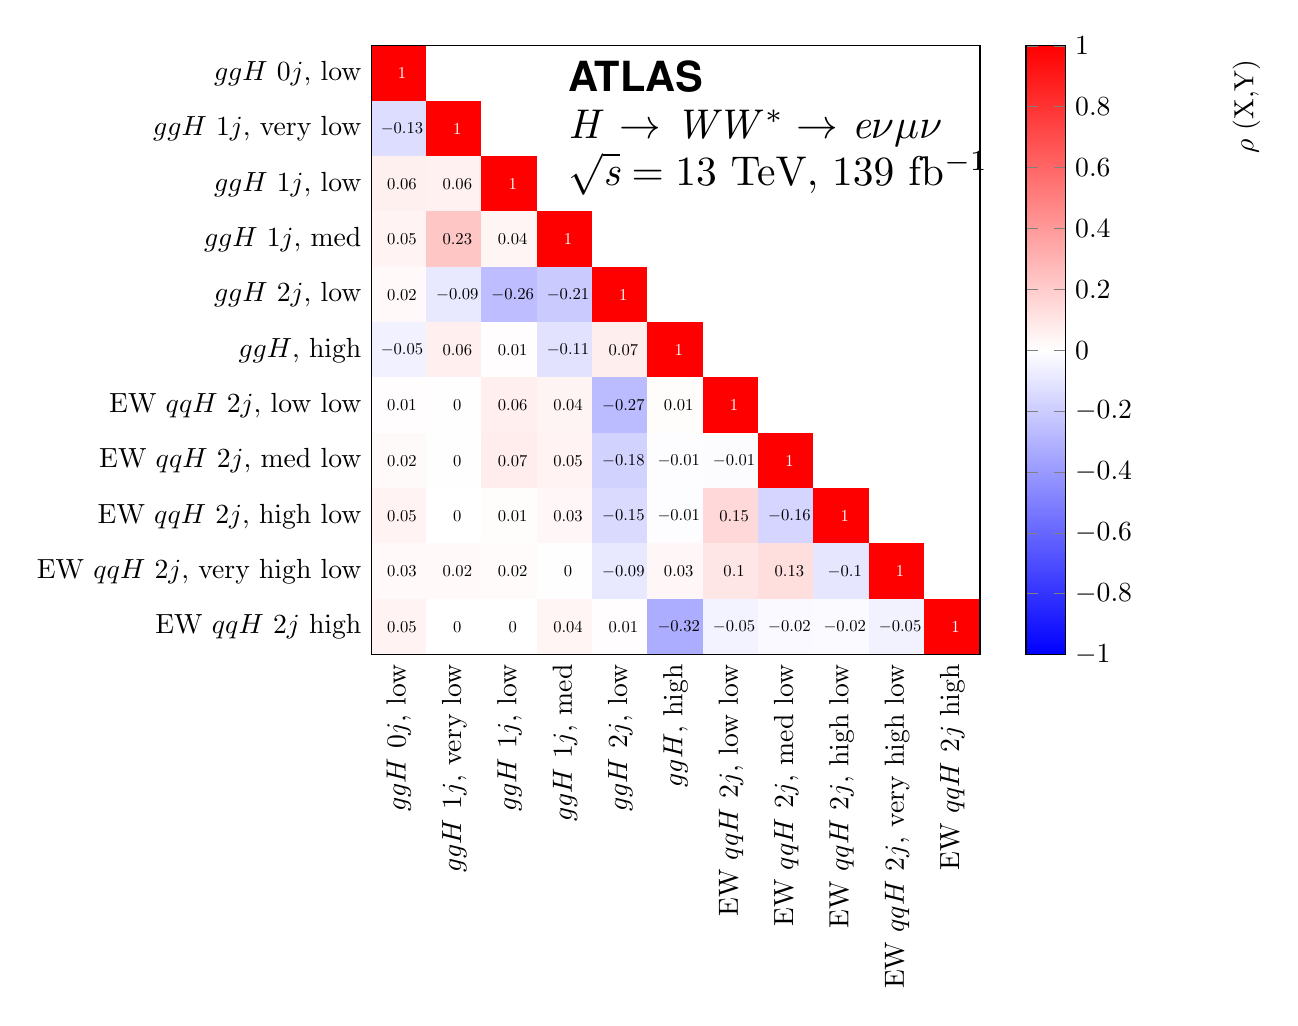
\begin{tikzpicture}
\begin{axis}[
    colormap={bluewhitered}{color=(blue) color=(white) color=(red)},
    clip=false,
    colorbar,
    colorbar style={
    ytick={-1,-0.8,...,1},
    ylabel={$\rho$ (X,Y)},
    ylabel style={
        at={(ticklabel cs:0.9)}
    },
    yticklabel style={
    text width=5em,
    ytick={-1,-0.8,...,1},
        tick style={draw=gray!}
        }
    },
    colormap name={bluewhitered},
   %  colormap/jet,
   % colorbar,
   % point meta min=0.0,
   % point meta max=0.2860,
   %  colorbar style={ height= 10 cm},xtick={0,0.286},
    % x=1em,
    % y=1em,
    x=2em,
    y=2em,
    xtick=data,
    ytick=data,
    ymin={$ggH~0j$, low \pTH},
    ymax={EW $qqH~2j$ high \pTH},
    xmin={$ggH~0j$, low \pTH},
    xmax={EW $qqH~2j$ high \pTH},
    y dir=reverse,
    % enlarge x limits={abs=0.5em},
    % enlarge y limits={abs=0.5em},
    enlarge x limits={abs=1em},
    enlarge y limits={abs=1em},
    point meta min=-1,
    point meta max=+1,
    % grid=both,
    major grid style={draw=none},
    visualization depends on={x\as\X},
    visualization depends on={y\as\Y},
    visualization depends on={correlations\as\Z},
    nodes near coords={\pgfmathtruncatemacro{\Z}
    {ifthenelse(\Y<\X,0,1)}
    \ifnum\Z=0
    \else\pgfmathprintnumber\pgfplotspointmeta\fi},
    % \ifthenelse{\X=+1}{\def\col{red}}{\def\col{black}},
    % every node near coord/.append style={anchor=center,scale=0.6,/pgf/number format/.cd,fixed,precision=2},
        % nodes near coord/.append={\pgfmathprintnumber\pgfplotspointmeta\,},
        % % ---------------------------------------------------------------------
        % % show `nodes near coords' but adapt the style so that values
        % % above a threshold get another style
        % % (adapted from <http://tex.stackexchange.com/a/141006/95441>)
        % % #1: the THRESHOLD after which we switch to a special display.
        nodes near coords black white/.style={
            small value/.style={
                text=black,
            },
            large value/.style={
                text=white,
            },
            every node near coord/.style={
                check for zero/.code={
                    \pgfmathfloatifflags{\pgfplotspointmeta}{0.0}{
                        % If meta=0, make the node a coordinate
                        % (which doesn't have text)
                        \pgfkeys{/tikz/coordinate}
                    }{
                        \begingroup
                        % this group is merely to switch to FPU locally.
                        % Might be unnecessary, but who knows.
                        \pgfkeys{/pgf/fpu}
                        \pgfmathparse{\pgfplotspointmeta<#1}
                        \global\let\result=\pgfmathresult
                        \endgroup
                        %
                        % simplifies debugging:
                        % \show\result
                        %
                        \pgfmathfloatcreate{0}{0.0}{0}
                        \let\ONE=\pgfmathresult
                        \ifx\result\ONE
                            \pgfkeysalso{/pgfplots/large value}
                        \else
                            \pgfkeysalso{/pgfplots/small value}
                        \fi
                    }
                },
                check for zero,
            }
        },
        % % asign a value to the new style thich is the threshold at which
        % % the two style `small value' or `large value' are used
        nodes near coords black white=0.9,
    every node near coord/.append style={font=\bfseries,anchor=center,scale=0.6,/pgf/number format/.cd,fixed,precision=2},
    minor tick num=1,
    symbolic x coords={{$ggH~0j$, low \pTH},{$ggH~1j$, very low \pTH},{$ggH~1j$, low \pTH},{$ggH~1j$, med \pTH},{$ggH~2j$, low \pTH},{$ggH$, high \pTH},{EW $qqH~2j$, low \mjj low \pTH},{EW $qqH~2j$, med \mjj low \pTH},{EW $qqH~2j$, high \mjj low \pTH},{EW $qqH~2j$, very high \mjj low \pTH},{EW $qqH~2j$ high \pTH}},
    symbolic y coords={{$ggH~0j$, low \pTH},{$ggH~1j$, very low \pTH},{$ggH~1j$, low \pTH},{$ggH~1j$, med \pTH},{$ggH~2j$, low \pTH},{$ggH$, high \pTH},{EW $qqH~2j$, low \mjj low \pTH},{EW $qqH~2j$, med \mjj low \pTH},{EW $qqH~2j$, high \mjj low \pTH},{EW $qqH~2j$, very high \mjj low \pTH},{EW $qqH~2j$ high \pTH}},
    axis on top,
    x tick label style={rotate=90},
    tick style={draw=none}
]
\addplot [matrix plot*,point meta=explicit,mesh/cols=11] table [meta=correlations] {
 x,  y,  correlations
 {$ggH~0j$, low \pTH} {$ggH~0j$, low \pTH} 1
 {$ggH~0j$, low \pTH} {$ggH~1j$, very low \pTH} -0.131324
 {$ggH~0j$, low \pTH} {$ggH~1j$, low \pTH}  0.059467
 {$ggH~0j$, low \pTH} {$ggH~1j$, med \pTH} 0.0490537
 {$ggH~0j$, low \pTH} {$ggH~2j$, low \pTH}  0.022738
 {$ggH~0j$, low \pTH} {$ggH$, high \pTH} -0.0546376
 {$ggH~0j$, low \pTH} {EW $qqH~2j$, low \mjj low \pTH} 0.0077486
 {$ggH~0j$, low \pTH} {EW $qqH~2j$, med \mjj low \pTH} 0.0211314
 {$ggH~0j$, low \pTH} {EW $qqH~2j$, high \mjj low \pTH}  0.0486984
 {$ggH~0j$, low \pTH} {EW $qqH~2j$, very high \mjj low \pTH} 0.0256006
 {$ggH~0j$, low \pTH} {EW $qqH~2j$ high \pTH} 0.0470472

 {$ggH~1j$, very low \pTH} {$ggH~0j$, low \pTH} 0
 {$ggH~1j$, very low \pTH} {$ggH~1j$, very low \pTH} 1
 {$ggH~1j$, very low \pTH} {$ggH~1j$, low \pTH}   0.0551626
 {$ggH~1j$, very low \pTH} {$ggH~1j$, med \pTH}  0.225791
 {$ggH~1j$, very low \pTH} {$ggH~2j$, low \pTH}   -0.0878372
 {$ggH~1j$, very low \pTH} {$ggH$, high \pTH}  0.0621163
 {$ggH~1j$, very low \pTH} {EW $qqH~2j$, low \mjj low \pTH}  0.00339789
 {$ggH~1j$, very low \pTH} {EW $qqH~2j$, med \mjj low \pTH}  0.0030145
 {$ggH~1j$, very low \pTH} {EW $qqH~2j$, high \mjj low \pTH}   0.00142807
 {$ggH~1j$, very low \pTH} {EW $qqH~2j$, very high \mjj low \pTH}   0.0224454
 {$ggH~1j$, very low \pTH} {EW $qqH~2j$ high \pTH} -0.00020307

 {$ggH~1j$, low \pTH}  {$ggH~0j$, low \pTH} 0
 {$ggH~1j$, low \pTH}  {$ggH~1j$, very low \pTH} 0
 {$ggH~1j$, low \pTH}  {$ggH~1j$, low \pTH}  1
 {$ggH~1j$, low \pTH}  {$ggH~1j$, med \pTH}  0.0382673
 {$ggH~1j$, low \pTH}  {$ggH~2j$, low \pTH}   -0.260164
 {$ggH~1j$, low \pTH}  {$ggH$, high \pTH}  0.00778543
 {$ggH~1j$, low \pTH}  {EW $qqH~2j$, low \mjj low \pTH}  0.0640812
 {$ggH~1j$, low \pTH}  {EW $qqH~2j$, med \mjj low \pTH}  0.0702857
 {$ggH~1j$, low \pTH}  {EW $qqH~2j$, high \mjj low \pTH}   0.014091
 {$ggH~1j$, low \pTH}  {EW $qqH~2j$, very high \mjj low \pTH}  0.0167539
 {$ggH~1j$, low \pTH}  {EW $qqH~2j$ high \pTH}  0.00113077

 {$ggH~1j$, med \pTH} {$ggH~0j$, low \pTH} 0
 {$ggH~1j$, med \pTH} {$ggH~1j$, very low \pTH} 0
 {$ggH~1j$, med \pTH} {$ggH~1j$, low \pTH}  0
 {$ggH~1j$, med \pTH} {$ggH~1j$, med \pTH} 1
 {$ggH~1j$, med \pTH} {$ggH~2j$, low \pTH}  -0.207511
 {$ggH~1j$, med \pTH} {$ggH$, high \pTH} -0.114735
 {$ggH~1j$, med \pTH} {EW $qqH~2j$, low \mjj low \pTH} 0.0425279
 {$ggH~1j$, med \pTH} {EW $qqH~2j$, med \mjj low \pTH} 0.0476515
 {$ggH~1j$, med \pTH} {EW $qqH~2j$, high \mjj low \pTH}  0.0336961
 {$ggH~1j$, med \pTH} {EW $qqH~2j$, very high \mjj low \pTH} 0.00431544
 {$ggH~1j$, med \pTH} {EW $qqH~2j$ high \pTH} 0.0390297

 {$ggH~2j$, low \pTH}  {$ggH~0j$, low \pTH} 0
 {$ggH~2j$, low \pTH}  {$ggH~1j$, very low \pTH} 0
 {$ggH~2j$, low \pTH}  {$ggH~1j$, low \pTH}  0
 {$ggH~2j$, low \pTH}  {$ggH~1j$, med \pTH} 0
 {$ggH~2j$, low \pTH}  {$ggH~2j$, low \pTH}  1
 {$ggH~2j$, low \pTH}  {$ggH$, high \pTH} 0.0669787
 {$ggH~2j$, low \pTH}  {EW $qqH~2j$, low \mjj low \pTH} -0.265444
 {$ggH~2j$, low \pTH}  {EW $qqH~2j$, med \mjj low \pTH} -0.176917
 {$ggH~2j$, low \pTH}  {EW $qqH~2j$, high \mjj low \pTH}  -0.145543
 {$ggH~2j$, low \pTH}  {EW $qqH~2j$, very high \mjj low \pTH} -0.0889487
 {$ggH~2j$, low \pTH}  {EW $qqH~2j$ high \pTH} 0.00671903

 {$ggH$, high \pTH} {$ggH~0j$, low \pTH} 0
 {$ggH$, high \pTH} {$ggH~1j$, very low \pTH} 0
 {$ggH$, high \pTH} {$ggH~1j$, low \pTH}  0
 {$ggH$, high \pTH} {$ggH~1j$, med \pTH} 0
 {$ggH$, high \pTH} {$ggH~2j$, low \pTH}  0
 {$ggH$, high \pTH} {$ggH$, high \pTH} 1
 {$ggH$, high \pTH} {EW $qqH~2j$, low \mjj low \pTH} 0.0119376
 {$ggH$, high \pTH} {EW $qqH~2j$, med \mjj low \pTH} -0.00631914
 {$ggH$, high \pTH} {EW $qqH~2j$, high \mjj low \pTH}  -0.0071606
 {$ggH$, high \pTH} {EW $qqH~2j$, very high \mjj low \pTH} 0.0303077
 {$ggH$, high \pTH} {EW $qqH~2j$ high \pTH} -0.322628

 {EW $qqH~2j$, low \mjj low \pTH} {$ggH~0j$, low \pTH} 0
 {EW $qqH~2j$, low \mjj low \pTH} {$ggH~1j$, very low \pTH} 0
 {EW $qqH~2j$, low \mjj low \pTH} {$ggH~1j$, low \pTH} 0
 {EW $qqH~2j$, low \mjj low \pTH} {$ggH~1j$, med \pTH} 0
 {EW $qqH~2j$, low \mjj low \pTH} {$ggH~2j$, low \pTH} 0
 {EW $qqH~2j$, low \mjj low \pTH} {$ggH$, high \pTH} 0
 {EW $qqH~2j$, low \mjj low \pTH} {EW $qqH~2j$, low \mjj low \pTH} 1
 {EW $qqH~2j$, low \mjj low \pTH} {EW $qqH~2j$, med \mjj low \pTH} -0.0093563
 {EW $qqH~2j$, low \mjj low \pTH} {EW $qqH~2j$, high \mjj low \pTH}  0.148795
 {EW $qqH~2j$, low \mjj low \pTH} {EW $qqH~2j$, very high \mjj low \pTH} 0.0993198
 {EW $qqH~2j$, low \mjj low \pTH} {EW $qqH~2j$ high \pTH} -0.0476769

 {EW $qqH~2j$, med \mjj low \pTH} {$ggH~0j$, low \pTH} 0
 {EW $qqH~2j$, med \mjj low \pTH} {$ggH~1j$, very low \pTH} 0
 {EW $qqH~2j$, med \mjj low \pTH} {$ggH~1j$, low \pTH} 0
 {EW $qqH~2j$, med \mjj low \pTH} {$ggH~1j$, med \pTH} 0
 {EW $qqH~2j$, med \mjj low \pTH} {$ggH~2j$, low \pTH} 0
 {EW $qqH~2j$, med \mjj low \pTH} {$ggH$, high \pTH} 0
 {EW $qqH~2j$, med \mjj low \pTH} {EW $qqH~2j$, low \mjj low \pTH} 0
 {EW $qqH~2j$, med \mjj low \pTH} {EW $qqH~2j$, med \mjj low \pTH} 1
 {EW $qqH~2j$, med \mjj low \pTH} {EW $qqH~2j$, high \mjj low \pTH}  -0.162325
 {EW $qqH~2j$, med \mjj low \pTH} {EW $qqH~2j$, very high \mjj low \pTH} 0.129734
 {EW $qqH~2j$, med \mjj low \pTH} {EW $qqH~2j$ high \pTH} -0.0214162


 {EW $qqH~2j$, high \mjj low \pTH}  {$ggH~0j$, low \pTH} 0
 {EW $qqH~2j$, high \mjj low \pTH}  {$ggH~1j$, very low \pTH} 0
 {EW $qqH~2j$, high \mjj low \pTH}  {$ggH~1j$, low \pTH} 0
 {EW $qqH~2j$, high \mjj low \pTH}  {$ggH~1j$, med \pTH} 0
 {EW $qqH~2j$, high \mjj low \pTH}  {$ggH~2j$, low \pTH} 0
 {EW $qqH~2j$, high \mjj low \pTH}  {$ggH$, high \pTH} 0
 {EW $qqH~2j$, high \mjj low \pTH}  {EW $qqH~2j$, low \mjj low \pTH} 0
 {EW $qqH~2j$, high \mjj low \pTH}  {EW $qqH~2j$, med \mjj low \pTH} 0
 {EW $qqH~2j$, high \mjj low \pTH}  {EW $qqH~2j$, high \mjj low \pTH}  1
 {EW $qqH~2j$, high \mjj low \pTH}  {EW $qqH~2j$, very high \mjj low \pTH} -0.0961078
 {EW $qqH~2j$, high \mjj low \pTH}  {EW $qqH~2j$ high \pTH} -0.0200312

 {EW $qqH~2j$, very high \mjj low \pTH} {$ggH~0j$, low \pTH} 0
 {EW $qqH~2j$, very high \mjj low \pTH} {$ggH~1j$, very low \pTH} 0
 {EW $qqH~2j$, very high \mjj low \pTH} {$ggH~1j$, low \pTH} 0
 {EW $qqH~2j$, very high \mjj low \pTH} {$ggH~1j$, med \pTH} 0
 {EW $qqH~2j$, very high \mjj low \pTH} {$ggH~2j$, low \pTH} 0
 {EW $qqH~2j$, very high \mjj low \pTH} {$ggH$, high \pTH} 0
 {EW $qqH~2j$, very high \mjj low \pTH} {EW $qqH~2j$, low \mjj low \pTH} 0
 {EW $qqH~2j$, very high \mjj low \pTH} {EW $qqH~2j$, med \mjj low \pTH} 0
 {EW $qqH~2j$, very high \mjj low \pTH} {EW $qqH~2j$, high \mjj low \pTH} 0
 {EW $qqH~2j$, very high \mjj low \pTH} {EW $qqH~2j$, very high \mjj low \pTH} 1
 {EW $qqH~2j$, very high \mjj low \pTH} {EW $qqH~2j$ high \pTH} -0.0513732

 {EW $qqH~2j$ high \pTH} {$ggH~0j$, low \pTH} 0
 {EW $qqH~2j$ high \pTH} {$ggH~1j$, very low \pTH} 0
 {EW $qqH~2j$ high \pTH} {$ggH~1j$, low \pTH} 0
 {EW $qqH~2j$ high \pTH} {$ggH~1j$, med \pTH} 0
 {EW $qqH~2j$ high \pTH} {$ggH~2j$, low \pTH} 0
 {EW $qqH~2j$ high \pTH} {$ggH$, high \pTH} 0
 {EW $qqH~2j$ high \pTH} {EW $qqH~2j$, low \mjj low \pTH} 0
 {EW $qqH~2j$ high \pTH} {EW $qqH~2j$, med \mjj low \pTH} 0
 {EW $qqH~2j$ high \pTH} {EW $qqH~2j$, high \mjj low \pTH} 0
 {EW $qqH~2j$ high \pTH} {EW $qqH~2j$, very high \mjj low \pTH} 0
 {EW $qqH~2j$ high \pTH} {EW $qqH~2j$ high \pTH} 1
};
\node (atlas) [above right, font={\fontfamily{phv}\fontseries{b}\selectfont},scale=1.5] at (rel axis cs:0.3,0.9) {ATLAS};
% \node (internal) [anchor=west,scale=1.5] at (atlas.east) {Internal};
\node (secondline)[above right,scale=1.5] at (rel axis cs:0.3,0.81) {\emph{H} $\to$ \emph{WW}$^{*} \to$ \emph{e$\nu\mu\nu$}};
\node (thirdline)[above right,scale=1.5] at (rel axis cs:0.3,0.73) {$\sqrt{\emph{s}} = 13$ TeV, 139 fb$^{-1}$};
%\node[rotate=90] at (120,100){$\rho$ (X,Y)};
\end{axis}
\end{tikzpicture}
% \end{document}

%\includegraphics[width=1.2\textwidth]{\paperfiguredir/CorrelationMatrix} % Only to be used for the figure extraction script
}
\caption{
  Correlations between the cross-section measurements in the 11 STXS bins for the \hwwenmn analysis.
  \label{fig:STXS-correlation}
}
\end{figure}

% Table with yields in each STXS SR (likely to go in auxiliary material)
%%%%%%%%%%%%%%%%%%%%%%%%%%%%%%%%%%%%####################################



% Table with STXS XSec measurements and their uncertainties
%%%%%%%%%%%%%%%%%%%%%%%%%%%%%%%%%%%%%%%%%%%%%%%%%%%%%%%%%%%%%%%%%%%%%%%%%%%%%

\begin{table}[htp]
  \caption{
    Best-fit values and uncertainties for the production cross section times $\hww$ branching fraction $({\sigma_i \cdot \mathcal{B}_{H \to WW^{\ast}}})$ in each STXS bin.
    }
  \begin{center}
  \small
   \renewcommand{\arraystretch}{1.5}
    \scalebox{0.90}{
    \begin{tabular}{l|rccccc|S[table-format=5,table-number-alignment=right]@{$\,\pm\,$}
                                    S[table-format=3,table-number-alignment=left]}
      \hline \hline
      \multirow{2}{*}{STXS bin $({\sigma_i \cdot \mathcal{B}_{H \to WW^{\ast}}})$} & \multicolumn{1}{c}{Value} & \multicolumn{5}{c|}{ Uncertainty [fb]} & \multicolumn{2}{c}{SM prediction} \\
                             &  \multicolumn{1}{c}{[fb]} &     Total                 & Stat.                       & Exp.\ Syst.                  & Sig.\ Theo.                  &    Bkg.\ Theo.    & \multicolumn{2}{c}{[fb]}   \\
\hline
\makecell[l]{\noalign{\vskip 2mm} \ggHZeroJ  \\ {\scriptsize \ggHZeroJMath}}                  & $7100$                    & $^{+ 950}_{-910}$           & $^{+480}_{-470}$          & $^{+570}_{-530}$            & $^{+320}_{-260}$            & $^{+490}_{-480}$          & 5870  & 390           \\ [0.4cm]
\makecell[l]{\noalign{\vskip 1mm}\ggHOneJVLowPt  \\ {\scriptsize \ggHOneJVLowPtMath}}          & $1140$                    & $^{+ 800}_{-820}$           & $^{+420}_{-410}$          & $^{+380}_{-380}$            & $^{+80\phantom{0}}_{-70}$   & $^{+570}_{-600}$          & 1400 &  190            \\ [0.4cm]
\makecell[l]{\ggHOneJLowPt  \\ {\scriptsize \ggHOneJLowPtMath}}                 & $540$                     & $^{+ 470}_{-470}$           & $^{+310}_{-310}$          & $^{+230}_{-230}$            & $^{+42\phantom{0}}_{-47}$   & $^{+270}_{-280}$          & 970  & 150             \\ [0.4cm]
\makecell[l]{\ggHOneJMedPt  \\ {\scriptsize \ggHOneJMedPtMath}}                 & $230$                     & $^{+ 130}_{-120}$           & $^{+100}_{-100}$ & $^{+60\phantom{0}}_{-60}$   & $^{+10\phantom{0}}_{-10}$   & $^{+50\phantom{0}}_{-50}$ & 160  & 30             \\ [0.4cm]
\makecell[l]{\ggHTwoJ  \\ {\scriptsize \ggHTwoJMath}}                     & $1610$                    & $^{+ 900}_{-890}$           & $^{+440}_{-440}$          & $^{+430}_{-420}$            & $^{+300}_{-150}$   & $^{+640}_{-650}$          & 1010  & 220             \\ [0.4cm]
\makecell[l]{\ggHHighPt  \\ {\scriptsize \ggHHighPtMath}}                  & $260$                     & $^{+ 100}_{-100}$           & $^{+80\phantom{0}}_{-80}$ & $^{+40\phantom{0}}_{-40}$   & $^{+40\phantom{0}}_{-20}$   & $^{+40\phantom{0}}_{-40}$ & 122 & 31             \\ [0.4cm]
\makecell[l]{\qqHLowMjj \\ {\scriptsize \qqHLowMjjMath}}                  & $6$                     & $^{+ 63\phantom{0}}_{-62}$  & $^{+46\phantom{0}}_{-42}$ & $^{+31\phantom{0}}_{-34}$   & $^{+11\phantom{0}}_{-14}$   & $^{+24\phantom{0}}_{-26}$ & 109 & 7             \\ [0.4cm]
\makecell[l]{\qqHMedMjj \\ {\scriptsize \qqHMedMjjMath}}                   & $31$                      & $^{+ 35\phantom{0}}_{-33}$  & $^{+30\phantom{0}}_{-27}$ & $^{+15\phantom{0}}_{-14}$   & $^{+8\phantom{0}}_{-7}$    & $^{+11\phantom{0}}_{-10}$ & 56 & 4             \\ [0.4cm]
\makecell[l]{\qqHHighMjj \\ {\scriptsize \qqHHighMjjMath}}                 & $60$                      & $^{+ 26\phantom{0}}_{-23}$  & $^{+23\phantom{0}}_{-21}$ & $^{+7\phantom{00}}_{-7}$    & $^{+9\phantom{00}}_{-5}$    & $^{+5\phantom{00}}_{-5}$  & 51 & 4            \\ [0.4cm]
\makecell[l]{\qqHVHighMjj \\ {\scriptsize \qqHVHighMjjMath}}          & $57$                      & $^{+ 20\phantom{0}}_{-18}$  & $^{+18\phantom{0}}_{-17}$ & $^{+5\phantom{00}}_{-5}$    & $^{+3\phantom{00}}_{-3}$    & $^{+4\phantom{00}}_{-4}$  & 50 & 4             \\ [0.4cm]
\makecell[l]{\qqHHighPt \\ {\scriptsize   \qqHHighPtMath}}                & $37$                      & $^{+ 16\phantom{0}}_{-14}$  & $^{+14\phantom{0}}_{-13}$ & $^{+4\phantom{00}}_{-3}$    & $^{+4\phantom{00}}_{-3}$    & $^{+3\phantom{00}}_{-3}$  & 32 & 1            \\ [0.4cm]
\hline
    \end{tabular}
    }
  \end{center}
  \label{tab:STXS-XSecs}
\end{table}




% Not sure if I want to have the NFs!
% \begin{table}[!h]
%     \centering
%     \renewcommand{\arraystretch}{1.6}
%       \caption{
%         Post-fit normalization factors which scale the corresponding estimated yields in the relevant signal region; the dash indicates where a MC-based normalization is used.
%         The quoted uncertainties include both the statistical and systematic contributions.
%       }
%       \label{tab:CRs_NF}
%     \scalebox{1.0}{
%     \begin{tabular}{c c c c}
%     \hline\hline
%     Category      & $WW$           &   $t\bar{t}/Wt$   & $Z/\gamma^{\ast}$   \\
%     \hline\hline
%     \ZeroJet ggF    &  $1.02^{+0.07}_{-0.07}$ &  $0.93^ {+0.22}_{-0.17}$ & $0.96^ {+0.07}_{-0.06}$ \\
%     \OneJet ggF    &  $0.85^{+0.16}_{-0.15}$ &  $1.05^ {+0.19}_{-0.16}$ & $0.98^ {+0.10}_{-0.09}$ \\
%     \TwoJet ggF  &  $0.81^{+0.34}_{-0.33}$ &  $0.96^ {+0.23}_{-0.18}$ & $0.98^ {+0.18}_{-0.17}$ \\
%     \TwoJet VBF  &  --                     &  $0.92^ {+0.33}_{-0.21}$ & $0.93^ {+0.23}_{-0.19}$ \\
%     \noalign{\vskip 1mm}
%     \hline\hline
%     \end{tabular}
%     }
%     \end{table}
    

\section{Conclusion}
\label{sec:conclusion}
\chapter{Conclusion}
\label{chap:conclusion}
% RESOURCES:
% https://www.nature.com/articles/s41567-020-01054-6.pdf
%The discovery of the Higgs boson in 2012 opened 

%Bernd comment: I wonder if you should re-iterate the discovery of the Higgs Boson and how it opened a new window in particle physics etc?"}
% After the discovery of the Higgs boson by the ATLAS and CMS experiments in 2012, an era of exploration of the properties of the Higgs boson began.
% The discovery of a particle consistent with the Higgs boson of the Standard Model (SM) by the ATLAS and CMS experiments in 2012 opened a new era of exploration.
After the discovery of a particle consistent with the Higgs boson of the Standard Model (SM) of particle physics by the ATLAS and CMS experiments in 2012, an era of exploration of the properties of the Higgs boson began.
%was a milestone in the history of particles physics. 
% The Higgs boson is a unique tool in the search for the fundamental laws of nature, as it is connected to many of the open fundamental questions the SM cannot answer.
% In the search for the fundamental laws of nature, the Higgs boson is a unique tool.
% It sits at the core of the Standard Model (SM), which is known to be incomplete, or merely an approximation of a more fundamental theory. 
Precise measurements of Higgs boson interactions allow for testing a broad range of SM predictions and are therefore of paramount interest.
It enables setting strong constraints on physics beyond the SM and may point to signs of new phenomena. % 
% or could point to signs of physics beyond the Standard Model.
%provides a promising path to find possible deviations from the SM. 
% This provides a promising path to the discovery of new phenomena. 
% To test the SM and find possible deviations of its predictions, a precise understanding of all Higgs boson processes is therefore crucial. 
%The precise understanding of Higgs boson processes is therefore a crucial task. 
%OR: The study of the Higgs boson is therefore one of the most important areas of research to test the SM and find its wholes. 
%Ten years after the discovery of the Higgs boson, no experimental signs of deviations of the SM have formed. 
%The physics program at the LHC provides a dataset unprecedented in size and well-suited for the study of Higgs boson processes. 

In this thesis, contributions to this endeavor were presented across different areas that build upon each other. 
First, the measurement of the noise term of the jet energy resolution (JER) was presented. 
This was performed for the first time for particle flow jets and is an important input to the calibration of the JER used in many physics analyses performed with the ATLAS experiment. 
The calibrations are also crucial for the results presented in the second and main part of this work: the measurements of the gluon fusion (ggF) and vector-boson fusion (VBF) production cross sections of the Higgs boson identified by its decay to a pair of $W$ bosons.

The analysis of \HWW\ decays was carried out using the full dataset collected by the ATLAS experiment during \RunTwo of the LHC, corresponding to 139\,\ifb\ proton-proton collisions at a center-of-mass energy of $\sqrt{s} = 13\,$TeV. 
Compared to the previous results from the ATLAS collaboration~\cite{HIGG-2016-07} that uses a partial \RunTwo dataset, the relative uncertainty on the measurements of the inclusive ggF and VBF production cross sections times branching fraction was reduced by almost 40\% and 60\%, respectively, yielding 
\begin{eqnarray*}
    \sigma_{\mathrm{ggF}} \cdot \mathcal{B}_{H \to WW^{\ast}} &=& 12.0 \pm 1.4~\mathrm{pb}, \,\text{and} \\
    \sigma_{\mathrm{VBF}} \cdot \mathcal{B}_{H \to WW^{\ast}} &=& 0.75\;^{+0.19}_{-0.16}~\mathrm{pb},
\end{eqnarray*}
which is in agreement with the SM predictions.
The measurement of the VBF production mode benefited significantly from the author's work on the development of a deep neural network that distinguishes the VBF, \HWW signal from the backgrounds.
This allowed observing the VBF production mode of the Higgs boson for the first time in the \HWW channel with a significance of $5.8\,\sigma$ above the background expectation, where $6.2\,\sigma$ were expected assuming the SM.
In addition, cross-section measurements of the ggF and VBF production mode have been performed in 11 separate kinematic regions, using the framework of Simplified Template Cross Sections (STXS). This probes the Higgs boson production in exclusive kinematic regions that have not been measured before with \HWW decays.
The results more firmly establish the Higgs boson in the SM, as they are all found to be compatible with the SM predictions.

The results from the \HWW analysis will be the baseline for future analyses and combinations, as well as reinterpretations such as in Effective Field Theories.
The author also suggested changes to the analysis strategy that could further improve the \HWW cross-section measurements, in particular in the analysis categories with two or more jets.

The measurements were already used as inputs to combined Higgs boson measurements~\cite{NaturePaper}, where they made an essential contribution. 
They contributed to some of the most precise measurements of inclusive Higgs boson production as well as to measurements of the kinematic properties of Higgs boson production.
% In particular, it led to the most precise measurement to date of the coupling of the Higgs boson to vector bosons yielding $\kappa_{V} = 1.035 \pm 0.031$, using the $\kappa$ framework~\cite{LHCHandbookV3}.
In particular, the input from the \HWW analysis drives the most precise measurement to date of the coupling of the Higgs boson to $W$ bosons, yielding $\kappa_{W} = 1.05 \pm 0.06$, using the $\kappa$ framework~\cite{LHCHandbookV3}.

These in-depth studies of some of the properties of the Higgs boson continue the highly successful Higgs boson physics program at the LHC and its experiments. 
So far, no deviations of the SM have been found. However, some of the uncertainties are still sizable and further measurements are needed to make progress in understanding the exact role the Higgs boson plays in nature. 

% using improved analysis strategies as, for example, suggested by the author of this thesis. 
% There is still room to improve the analysis strategies, as studied by the author to further improv the \HWW cross-section measurements.
% For the \HWW analysis, for example, the author suggested alternative analysis strategies that could further improve the \HWW cross-section measurements. 
%, which are expected to make a substantial impact on constraining theories beyond the SM and may open doors to new phenomena.

% \TDinote{}{Will be one of the goals in the future to combine measurements to get the most out of the data}
% Furthermore, the analysis presented was crucial input to combined Higgs boson measurements that combine analyses of multiple Higgs boson processes. In particular, the \HWW analysis is the most important input to the measurement of the coupling of the Higgs boson to vector-bosons, determined to be $\kappa_V = 1.035 \pm 0.031$.
% The data analysis of the full \RunTwo dataset has not been fully completed. 
% More results are imminent, aiming at an even more comprehensive experimental map of Higgs boson processes and other phenomena. 
% Looking ahead, the data analysis of the full \RunTwo dataset has not yet been completed and consolidated results are expected in the coming years.
Looking ahead, the data taking at the LHC continued with \RunThr in July 2022, operating under similar data taking conditions as \RunTwo. 
With more data, as well as more sophisticated analysis strategies, the properties of the Higgs boson can be studied at even higher precision and new Higgs boson processes will become experimentally accessible. 
This will allow rare Higgs boson processes to be investigated, for example, the $H \to \mu\mu$ or $H \to Z\gamma$ decays or the coupling of the Higgs boson to itself.
%The latter includes the production of di-Higgs processes, allowing to measure , and other rare Higgs processes. 
% room for new phenomena beyond the SM
Even more potential to measure these key properties and other phenomena is expected from the High-Luminosity LHC and its upgraded experiments after 2029.
%, which are currently estimated to collect about 20 times the amount of data recorded during \RunTwo of the LHC. 
The study of the Higgs boson and its unique properties will continue to be of utmost importance, guiding the particle physics community in the search for the fundamental laws of nature. 

% At the time of writing, in between \RunTwo and \RunThr of the LHC, it would be a miss not to mention that many physicists had hoped for more discoveries of fundamental particles at the LHC than have been reported so far.
% Yet, no experimental signs of deviations of the SM have formed.
% % In a way, this is the very nature of fundamental physics, which is driven by curiosity and can never be too certain of what lies ahead, making it one of the most exciting research fields. 
% The current situation in particle physics, i.e. the discovery of the Higgs boson and the exclusion of the existence of many other fundamental particles that were predicted by theoretical models, most notably the ones predicted by supersymmetric models, requires a close examination of existing theories. This special circumstance can also be considered a unique opportunity to stimulate new groundbreaking ideas.
% %and to revisit the most fundamental principles. 
% The study of the Higgs boson and its unique properties will guide the physics community in this pursuit.
% %, striving to find hints of new phenomena through precision measurements. 
% With a wealth of physics data yet to be collected at the LHC and new research facilities in planning, substantial progress in this area is expected in the years to come. 
% If scientists continue to push beyond the boundaries of technology and collaborative practices, as has been so successfully demonstrated by the LHC program, new insights will be gained that could shed light on the open mysteries of the universe and bring humanity closer to having a complete description of the fundamental laws of nature. 

%could potentially disrupt our entire understanding of the universe and 
% Guided by the data from full \RunTwo of the LHC, it is important to set out new research directions.
% Since no signs of physics beyond the SM have been found to date, it is a crucial task to deepen our understanding of the physics we already know. 
% A prime study is the one of the Higgs boson, which sits at the core of the SM and builds an important building block for many theories beyond the SM.
% This thesis presented the study of Higgs bosons in their decays to $W$ bosons, providing measurements of unprecedented precision as well as resolution. 
% \TDinote{}{Mention machine learning to close the circle with the intro!}
% The analysis will be the baseline for many future combinations and reinterpretations such as in Effective Field Theories. 
% The results were also crucial input to combined Higgs boson measurements that provide a comprehensive study of Higgs boson processes.

% suggest that the SM is merely an approximation of a more fundamental theory. 
% While the physics program at the LHC has been a great success, delivering results with unprecedented precision and constraining many of the theories beyond the SM, ...
% pushing the boundaries of technology and collaborative efforts and leaving no doubt about a huge experimental success.

% Nevertheless, the physics community seems to be slowly growing impatient, and it would be a miss not to mention that several physicists had hoped for the LHC program to provide more answers than it has delivered to date. 
% Several questions remain to be answered and no clear hints on where new physics may hide have been provided.
% In the case of theories beyond the SM such as supersymmetry, for example, it may be deemed disappointing rather than a success that no signs of it being realized in nature have been found so far. 
% In fact, this seems to be how it is often perceived from outside the physics community. 
% Whatever the framing might be, the LHC and its experiments have delivered outstanding results, pushing the boundaries of technology and collaborative efforts and leaving no doubt about a huge experimental success.
% In fact, if looking at physics for what it is, a fundamentally data-driven science, the LHC has done exactly as promised, providing a rich dataset to be explored. 
% From an experimentalist point of view, there is no doubt that the LHC including his experiments were a huge success.
%At the time of writing, 10 years after the Higgs boson discovery, it is therefore a good time to look at physics for what it is, a fundamentally data-driven science.

% % % % %-------------------------------------------------------------------------------
\chapter{Summary of Combined Measurements of Higgs Boson Interactions}
% \chapter{$H\rightarrow W^{\pm}W^{\mp^*}$ Cross-Sections Measurements}
% \chapter{Measurements of $H\rightarrow W^{\pm}W^{\mp^*}$ Cross sections}
\label{chap:comb}

The analysis of \HWW decays presented in \cref{chap:hww} is combined with other measurements of Higgs boson production and decays. This is crucial to probe every aspect of the rich phenomenology of Higgs boson physics (see \cref{chap:higgs}).
The results from the ATLAS collaboration are published in \ccite{NaturePaper} and as the title of the paper states establish a ``detailed map of Higgs boson interactions [\ldots] ten years after the discovery''. 
Together with similar measurements performed by the CMS collaboration~\cite{CMSNaturePaper} they represent the most precise and comprehensive measurements of the properties of the Higgs boson to date.
This chapter summarizes the results of the ATLAS collaboration, highlighting the impact of the \HWW analysis.
All measurements are found to be consistent with the SM expectations, thereby setting strong constraints on couplings to new particles beyond the SM.  

\section{Input Measurements and Fit Procedure}
The combined measurement is performed using the results of the analyses of various Higgs boson decay modes.
This includes the diboson decay modes: \HZZ, $H \to \gamma\gamma$, \HWW, and $H \to Z\gamma$; as well as the fermion decay modes: $H \to b\bar{b}$, $H \to \tau\bar{\tau}$, $H \to \mu\mu$, and $H \to c\bar{c}$. 
Different Higgs boson production modes are considered for each analysis including ggF, VBF, $VH$, $t\bar{t}H$, $tH$, and $bbH$. 
Most input measurements use the full set of \RunTwo data recorded by the ATLAS experiment at the LHC, corresponding to 139\ifb.

The combined measurements are performed by fitting a combined likelihood formed by the product of the likelihood function of each of the input measurements. 
The systematic uncertainties affecting multiple measurements are treated coherently in the combined fit to take into account the correlations between the NPs. 
Several combined fits are performed, testing different scenarios that differ, for example, in the definition of signal strengths in the likelihood.

% \section{Global Signal Strength Measurement}
% %%%%%%%%%%%%%%%%%%%%%%%%%%%%%%%%%%%%%%%

\section{Cross-Section Measurements}
When assuming that all production and decay processes scale with the same signal strength $\mu$, the fully inclusive Higgs boson signal strength is measured to be 
\begin{equation*}
   \mu =1.05 \pm 0.06 = 1.05\pm 0.03\, (\text{stat.})\, \pm 0.03\, (\text{exp.})\, \pm 0.04\, (\text{sig.\ th.})\, \pm 0.02\, (\text{bkg.\ th.}).
\end{equation*}

%%%%%%%%%%%%%%%%%%%%%%%%%%%%%%%%%%%%%%%
% Prod mode cross section
The cross sections of the different Higgs boson production modes times branching fraction are measured for specific combinations of production and decay processes. 
The results of a combined fit are shown in \cref{fig:prod-per-channel} and reveal the varying precision with which different Higgs boson processes have been measured to date. 
The contribution from the \HWW\ analysis is among the most important for the measurement of the ggF and VBF production modes.
%As can be seen, 
\begin{figure}
  \newImageResizeCustom{1}{figures/theory/higgs-measurements/fig4.pdf}
  \caption{Ratio of observed rate to predicted SM event rate for different combinations of
  Higgs boson production and decay processes. The horizontal bar on each point denotes the 68\% confidence interval. The narrow grey bands indicate the theory uncertainties in the SM cross section times the branching
fraction predictions. The $p$-value for compatibility of the measurement and the SM prediction is
72\%. Figure and caption taken from \ccite{NaturePaper}.}
  \label{fig:prod-per-channel}
\end{figure}
%%%%%%%%%%%%%%%%%%%%%%%%%%%%%%%%%%%%%%%%%%
% Decay fractions
% \todo{Maybe putting the decay fraction results is not necessary here!}
% The Higgs decay branching fractions can be measured by fixing the production mode cross section to the respective SM expectation and assuming that there are no non-SM decays. The results can be seen in \cref{fig:br-per-channel}.

%%%%%%%%%%%%%%%%%%%%%%%%%%%%%%%%%%%%%%%%%%
% - Latest STXS combination (from nature)
The kinematic properties of Higgs boson production are measured following the Stage 1.2 STXS scheme. 
The results are shown in \cref{fig:stxs-stage12}. 
The classification of Higgs boson production into 5 classes ($t\bar{t}H$, $tH$, $qq\to Hqq$, $pp\to VH$, and $gg\to H$) is detailed in \ccite{NaturePaper}. 
In particular, the measurements of $qq\to Hqq$ production at large \mjj benefit significantly from the input of the \HWW analysis. 
\TDinote{}{Messungen ergaenzen sich nicely gegenseitig.}
% From nature paper
% Higgs boson production is first classified according to the nature of the initial state and the associated particles, the latter including the decay products of $W$ and $Z$ bosons if they are present. These classes are: $t\bar{t}H$ and $tH$ processes; $qq'\to Hqq'$ processes, with contributions from both VBF and quark-initiated $VH$ (where $V=W, Z$) production with a hadronic decay of the vector boson; $pp\to VH$ production with a leptonic decay of the vector boson ($V(\ell\ell,\ell\nu)H$), including $gg\to ZH \to \ell\ell H$ production; and finally the ggF process combined with $gg\to ZH \to q\bar{q}H$ production to form a single $gg\to H$ process. The contribution of the $b\bar{b}H$ production process is taken into account as a $1\%$~\cite{YR4} increase of the \ggtoH\ yield in each kinematic region, since the acceptances for both processes are similar for all input analyses~\cite{YR4}.

\begin{figure}
  \newImageResizeCustom{1}{figures/theory/higgs-measurements/fig8.pdf}
  \caption{Observed and predicted Higgs boson production cross sections in different
  kinematic regions. The vertical bar on each point denotes the 68\% confidence interval. The $p$-value for compatibility of the combined measurement and the SM prediction is 94\%. Kinematic regions are defined separately for each production process, based on the jet multiplicity, the transverse momentum of the Higgs ($p_{\textrm{T}}^H$) and vector bosons ($p_{\textrm{T}}^W$ and $p_{\textrm{T}}^Z$) and the two-jet invariant mass ($m_{jj}$).
The `VH-enriched' and `VBF-enriched' regions with the respective requirements of $m_{jj}\in[60, 120)$ \GeV\ and $m_{jj}\notin[60,120)$ \GeV\ are enhanced in signal events from $VH$ and VBF productions, respectively. Figure and caption taken from \ccite{NaturePaper}.
  }
  \label{fig:stxs-stage12}
\end{figure}

\section{Higgs Boson Coupling Strenghts}
% The couplings of the Higgs boson to individual particles can be measured by parametrizing the cross sections and branching fractions for the individual Higgs boson processes in terms of coupling-strength modifiers, $\kappa$, following the $\kappa$ framework~\cite{LHCHandbookV3}. 
% For a production (decay) via the coupling to a given particle $p$, the modifier $\kappa_p$ is defined as $\kappa_p^2 = \sigma_p / \sigma_p^\text{SM}$ ($\kappa_p^2 = \Gamma_p/\Gamma_p^\text{SM}$), where $\Gamma_p$ is the partial decay width into a pair of particles $p$.\cite{NaturePaper}
%Different statistical models with varying assumptions that are detailed in \cite{NaturePaper} may be considered. 
The couplings of the Higgs boson to individual particles are measured for different scenarios following the $\kappa$ framework introduced in \cref{subsec:coupling-measurements}.
Assuming that there are only SM processes that interact exactly as predicted, and independently measuring coupling-strength modifiers for all included particles ($\kappa_W$, $\kappa_Z$, $\kappa_t$, $\kappa_b$, $\kappa_c$, $\kappa_\tau$, and $\kappa_\mu$), the results can be visualized as shown in \cref{fig:h-couplings}. 
This finds good consistency of the internal structure of the SM, but at the same time reveals that the uncertainties on the measurements are still sizable. 
The $\kappa_W$ modifier is measured with relative uncertainties of about 5-10\%, depending on the model assumed. 
This measurement is largely driven by the VBF, \HWW analysis, because it is sensitive to $\kappa_W$ in both the production and decay mode.
The VBF production mode is parametrized as $\kappa_\mathrm{VBF}^2 = 0.733 \kappa^2_W + 0.267 \kappa^2_Z$ in the combined measurement.

If the measurement is performed using only two independent coupling-strength modifiers, one for the vector bosons, $\kappa_V = \kappa_W = \kappa_Z$, and one for all fermions, $\kappa_F$, the results are $\kappa_V = 1.035 \pm 0.031$ and $\kappa_F = 0.95 \pm 0.05$. 
%and Higgs boson to fermion coupling, $\kappa_{F}$, are measured with a relative uncertainty of the order of 10\% and 20\%, respectively. 
% The VBF, \HWW analysis provides the most sensitive input to measure both $\kappa_W$ and $\kappa_V$, since the $HW$ vertex appears twice in the diagram. The VBF production mode enters the parametrization in the $\kappa$ framework (\cref{eq:kappa-parametrization}) as $\kappa_\mathrm{VBF}^2 = 0.733 \kappa^2_W + 0.267 \kappa^2_Z$~\cite{NaturePaper}. 
\begin{figure}
  \newImageResizeCustom{0.7}{figures/theory/higgs-measurements/fig6_paper.pdf}
  \caption{
    Reduced Higgs boson coupling strength modifiers and their uncertainties. They are defined as $\kappa_F \cdot m_F / \text{vev}$ for fermions
($F=t,b,\tau,\mu$) and $\sqrt{\kappa_V}\cdot m_V/\text{vev}$ for vector bosons as a
function of their masses $m_F$ and $m_V$. Two fit scenarios with $\kappa_c =
\kappa_t$ (colored circle markers), or $\kappa_c$ left free-floating in the fit (grey
cross markers) are shown. Loop-induced processes are assumed to have the SM structure, and Higgs boson decays to non-SM particles are not allowed. The vertical bar on each point denotes the 68\% confidence interval. The $p$-value for compatibility of the combined measurement and the SM prediction are 56\% and 65\% for the respective scenarios. The lower panel shows the values of the coupling strength modifiers. The grey arrow points in the direction of the best-fit value and the corresponding grey uncertainty bar extends beyond the lower panel range. Figure and caption taken from \ccite{NaturePaper}.}
  \label{fig:h-couplings}
\end{figure}


\bookmarksetup{startatroot}
% % % % %-------------------------------------------------------------------------------
\chapter{Conclusion}
\label{chap:conclusion}
% RESOURCES:
% https://www.nature.com/articles/s41567-020-01054-6.pdf
%The discovery of the Higgs boson in 2012 opened 

%Bernd comment: I wonder if you should re-iterate the discovery of the Higgs Boson and how it opened a new window in particle physics etc?"}
% After the discovery of the Higgs boson by the ATLAS and CMS experiments in 2012, an era of exploration of the properties of the Higgs boson began.
% The discovery of a particle consistent with the Higgs boson of the Standard Model (SM) by the ATLAS and CMS experiments in 2012 opened a new era of exploration.
After the discovery of a particle consistent with the Higgs boson of the Standard Model (SM) of particle physics by the ATLAS and CMS experiments in 2012, an era of exploration of the properties of the Higgs boson began.
%was a milestone in the history of particles physics. 
% The Higgs boson is a unique tool in the search for the fundamental laws of nature, as it is connected to many of the open fundamental questions the SM cannot answer.
% In the search for the fundamental laws of nature, the Higgs boson is a unique tool.
% It sits at the core of the Standard Model (SM), which is known to be incomplete, or merely an approximation of a more fundamental theory. 
Precise measurements of Higgs boson interactions allow for testing a broad range of SM predictions and are therefore of paramount interest.
It enables setting strong constraints on physics beyond the SM and may point to signs of new phenomena. % 
% or could point to signs of physics beyond the Standard Model.
%provides a promising path to find possible deviations from the SM. 
% This provides a promising path to the discovery of new phenomena. 
% To test the SM and find possible deviations of its predictions, a precise understanding of all Higgs boson processes is therefore crucial. 
%The precise understanding of Higgs boson processes is therefore a crucial task. 
%OR: The study of the Higgs boson is therefore one of the most important areas of research to test the SM and find its wholes. 
%Ten years after the discovery of the Higgs boson, no experimental signs of deviations of the SM have formed. 
%The physics program at the LHC provides a dataset unprecedented in size and well-suited for the study of Higgs boson processes. 

In this thesis, contributions to this endeavor were presented across different areas that build upon each other. 
First, the measurement of the noise term of the jet energy resolution (JER) was presented. 
This was performed for the first time for particle flow jets and is an important input to the calibration of the JER used in many physics analyses performed with the ATLAS experiment. 
The calibrations are also crucial for the results presented in the second and main part of this work: the measurements of the gluon fusion (ggF) and vector-boson fusion (VBF) production cross sections of the Higgs boson identified by its decay to a pair of $W$ bosons.

The analysis of \HWW\ decays was carried out using the full dataset collected by the ATLAS experiment during \RunTwo of the LHC, corresponding to 139\,\ifb\ proton-proton collisions at a center-of-mass energy of $\sqrt{s} = 13\,$TeV. 
Compared to the previous results from the ATLAS collaboration~\cite{HIGG-2016-07} that uses a partial \RunTwo dataset, the relative uncertainty on the measurements of the inclusive ggF and VBF production cross sections times branching fraction was reduced by almost 40\% and 60\%, respectively, yielding 
\begin{eqnarray*}
    \sigma_{\mathrm{ggF}} \cdot \mathcal{B}_{H \to WW^{\ast}} &=& 12.0 \pm 1.4~\mathrm{pb}, \,\text{and} \\
    \sigma_{\mathrm{VBF}} \cdot \mathcal{B}_{H \to WW^{\ast}} &=& 0.75\;^{+0.19}_{-0.16}~\mathrm{pb},
\end{eqnarray*}
which is in agreement with the SM predictions.
The measurement of the VBF production mode benefited significantly from the author's work on the development of a deep neural network that distinguishes the VBF, \HWW signal from the backgrounds.
This allowed observing the VBF production mode of the Higgs boson for the first time in the \HWW channel with a significance of $5.8\,\sigma$ above the background expectation, where $6.2\,\sigma$ were expected assuming the SM.
In addition, cross-section measurements of the ggF and VBF production mode have been performed in 11 separate kinematic regions, using the framework of Simplified Template Cross Sections (STXS). This probes the Higgs boson production in exclusive kinematic regions that have not been measured before with \HWW decays.
The results more firmly establish the Higgs boson in the SM, as they are all found to be compatible with the SM predictions.

The results from the \HWW analysis will be the baseline for future analyses and combinations, as well as reinterpretations such as in Effective Field Theories.
The author also suggested changes to the analysis strategy that could further improve the \HWW cross-section measurements, in particular in the analysis categories with two or more jets.

The measurements were already used as inputs to combined Higgs boson measurements~\cite{NaturePaper}, where they made an essential contribution. 
They contributed to some of the most precise measurements of inclusive Higgs boson production as well as to measurements of the kinematic properties of Higgs boson production.
% In particular, it led to the most precise measurement to date of the coupling of the Higgs boson to vector bosons yielding $\kappa_{V} = 1.035 \pm 0.031$, using the $\kappa$ framework~\cite{LHCHandbookV3}.
In particular, the input from the \HWW analysis drives the most precise measurement to date of the coupling of the Higgs boson to $W$ bosons, yielding $\kappa_{W} = 1.05 \pm 0.06$, using the $\kappa$ framework~\cite{LHCHandbookV3}.

These in-depth studies of some of the properties of the Higgs boson continue the highly successful Higgs boson physics program at the LHC and its experiments. 
So far, no deviations of the SM have been found. However, some of the uncertainties are still sizable and further measurements are needed to make progress in understanding the exact role the Higgs boson plays in nature. 

% using improved analysis strategies as, for example, suggested by the author of this thesis. 
% There is still room to improve the analysis strategies, as studied by the author to further improv the \HWW cross-section measurements.
% For the \HWW analysis, for example, the author suggested alternative analysis strategies that could further improve the \HWW cross-section measurements. 
%, which are expected to make a substantial impact on constraining theories beyond the SM and may open doors to new phenomena.

% \TDinote{}{Will be one of the goals in the future to combine measurements to get the most out of the data}
% Furthermore, the analysis presented was crucial input to combined Higgs boson measurements that combine analyses of multiple Higgs boson processes. In particular, the \HWW analysis is the most important input to the measurement of the coupling of the Higgs boson to vector-bosons, determined to be $\kappa_V = 1.035 \pm 0.031$.
% The data analysis of the full \RunTwo dataset has not been fully completed. 
% More results are imminent, aiming at an even more comprehensive experimental map of Higgs boson processes and other phenomena. 
% Looking ahead, the data analysis of the full \RunTwo dataset has not yet been completed and consolidated results are expected in the coming years.
Looking ahead, the data taking at the LHC continued with \RunThr in July 2022, operating under similar data taking conditions as \RunTwo. 
With more data, as well as more sophisticated analysis strategies, the properties of the Higgs boson can be studied at even higher precision and new Higgs boson processes will become experimentally accessible. 
This will allow rare Higgs boson processes to be investigated, for example, the $H \to \mu\mu$ or $H \to Z\gamma$ decays or the coupling of the Higgs boson to itself.
%The latter includes the production of di-Higgs processes, allowing to measure , and other rare Higgs processes. 
% room for new phenomena beyond the SM
Even more potential to measure these key properties and other phenomena is expected from the High-Luminosity LHC and its upgraded experiments after 2029.
%, which are currently estimated to collect about 20 times the amount of data recorded during \RunTwo of the LHC. 
The study of the Higgs boson and its unique properties will continue to be of utmost importance, guiding the particle physics community in the search for the fundamental laws of nature. 

% At the time of writing, in between \RunTwo and \RunThr of the LHC, it would be a miss not to mention that many physicists had hoped for more discoveries of fundamental particles at the LHC than have been reported so far.
% Yet, no experimental signs of deviations of the SM have formed.
% % In a way, this is the very nature of fundamental physics, which is driven by curiosity and can never be too certain of what lies ahead, making it one of the most exciting research fields. 
% The current situation in particle physics, i.e. the discovery of the Higgs boson and the exclusion of the existence of many other fundamental particles that were predicted by theoretical models, most notably the ones predicted by supersymmetric models, requires a close examination of existing theories. This special circumstance can also be considered a unique opportunity to stimulate new groundbreaking ideas.
% %and to revisit the most fundamental principles. 
% The study of the Higgs boson and its unique properties will guide the physics community in this pursuit.
% %, striving to find hints of new phenomena through precision measurements. 
% With a wealth of physics data yet to be collected at the LHC and new research facilities in planning, substantial progress in this area is expected in the years to come. 
% If scientists continue to push beyond the boundaries of technology and collaborative practices, as has been so successfully demonstrated by the LHC program, new insights will be gained that could shed light on the open mysteries of the universe and bring humanity closer to having a complete description of the fundamental laws of nature. 

%could potentially disrupt our entire understanding of the universe and 
% Guided by the data from full \RunTwo of the LHC, it is important to set out new research directions.
% Since no signs of physics beyond the SM have been found to date, it is a crucial task to deepen our understanding of the physics we already know. 
% A prime study is the one of the Higgs boson, which sits at the core of the SM and builds an important building block for many theories beyond the SM.
% This thesis presented the study of Higgs bosons in their decays to $W$ bosons, providing measurements of unprecedented precision as well as resolution. 
% \TDinote{}{Mention machine learning to close the circle with the intro!}
% The analysis will be the baseline for many future combinations and reinterpretations such as in Effective Field Theories. 
% The results were also crucial input to combined Higgs boson measurements that provide a comprehensive study of Higgs boson processes.

% suggest that the SM is merely an approximation of a more fundamental theory. 
% While the physics program at the LHC has been a great success, delivering results with unprecedented precision and constraining many of the theories beyond the SM, ...
% pushing the boundaries of technology and collaborative efforts and leaving no doubt about a huge experimental success.

% Nevertheless, the physics community seems to be slowly growing impatient, and it would be a miss not to mention that several physicists had hoped for the LHC program to provide more answers than it has delivered to date. 
% Several questions remain to be answered and no clear hints on where new physics may hide have been provided.
% In the case of theories beyond the SM such as supersymmetry, for example, it may be deemed disappointing rather than a success that no signs of it being realized in nature have been found so far. 
% In fact, this seems to be how it is often perceived from outside the physics community. 
% Whatever the framing might be, the LHC and its experiments have delivered outstanding results, pushing the boundaries of technology and collaborative efforts and leaving no doubt about a huge experimental success.
% In fact, if looking at physics for what it is, a fundamentally data-driven science, the LHC has done exactly as promised, providing a rich dataset to be explored. 
% From an experimentalist point of view, there is no doubt that the LHC including his experiments were a huge success.
%At the time of writing, 10 years after the Higgs boson discovery, it is therefore a good time to look at physics for what it is, a fundamentally data-driven science.

%-------------------------------------------------------------------------------
\clearpage
\addcontentsline{toc}{part}{Appendix}
\appendix
\renewcommand{\chaptermark}[1]{\markboth{\MakeUppercase{Appendix \hfill \chaptername\ \thechapter.\ #1}}{}}
\part*{Appendix}

% -------------------------------------------------------------------------------

\chapter{Development of the VBF DNN}


\section{Software suite for the development of the VBF DNN}
\label{app:dnn:software-suite}
The software used for the development of the DNN is based on industry-standard state-of-the-art ML libraries. 
The entire workflow is based on Docker images that provide the necessary packages that are all built with a Python frontend. The simulated MC samples provided centrally within the ATLAS collaboration are first transformed in order to remove the ATLAS software dependencies and make them easily useable with open-source ML libraries. The data is then stored in hdf5 format, and handled with the numpy and pandas packages. The training is performed using Keras and TensorFlow. The scikit-learn library is included in the training, and the matplotlib package is used for data visualization. The final DNN model is stored in JSON format and deployed in the \HWW\ analysis using the C++ based LightWeight Tagger Neural Network (lwtnn) package [148].
\todo{REFERENCES!}
\todo{Mention FreeForestML}


\section{Optimization studies for the development of the VBF DNN}
\label{app:dnn:opt-studies}

Different optimization studies for the VBF DNN were performed during the course of the author's PhD thesis.
The following studies were performed with an earlier version of the DNN training setup, including an earlier version of the training data. For this reason, the absolute values of $Z0$(40 bins) are not necessarily comparable with other results presented in this thesis. However, they are perfectly suitable for drawing conclusions when being compared against each other.

Many sets of observables were studied for use as DNN input variables.
As baseline, the set of variables that was used in the BDT-based analysis of the previous iteration of the \HWW\ measurement \cite{HIGG-2016-07} is chosen, comprising in total 8 variables.
The most important comparisons of the performances of models using an increasing number of variables are shown in \cref{tab:input-var-opt}.
Comparing the baseline to the results labelled ``S1'' shows significant improvements. This is an indication that the DNN exploits the correlations between the single $m_{\ell_\alpha j_\beta}$ (with $\alpha, \beta = 1, 2$) and other observables. 
Although the discrimination power of \pTjone and \pTjtwo in linear dimension is limited, they also introduce a significant performance improvement when being included (``S2''). The same is true for the \pTjthree observable (``S3''), which adds information about whether a third jet is present in the event. 
The final variable that was added and showed benefits is \METSig (``S4''). This observable has only recently been developed for use in the ATLAS collaboration \cite{ATLAS-CONF-2018-038} and is a strong discriminant between events with real undetected high-\pT particles and events where the \MET is the result of resolution effects. 
Overall the significance metric $Z0$(40 bins) improves by a maximum of almost 50\% when comparing the baseline with the best performing set.
These results motivate the use of the 15 input variables that correspond to the set labelled ``S4'' in \cref{tab:input-var-opt}.
In addition to the comparisons shown, several other observables were studied but did not lead to further improvements. 
These tests included (i) using the $C_\ell$ observable separately instead of the sum for both leptons, (ii) using \MET instead of \METSig, and (iii) using the \pT of both leptons on top of the other 15 variables.
Furthermore, the performance of DNN models trained with all 15 variables except one was studied. It was seen, that all of the chosen 15 variables provide discrimination power, although dropping highly correlated observables such as \mjj and \dyjj did not show strong performance losses.

The physics-motivated optimization of the input variables was followed by the rather technical optimization of the neural network architecture. 
The performances of different setups are shown in \cref{tab:architecture-opt}. All results are very similar to each other. Among the best performing architectures, the one with the least layers is chosen, which corresponds to the architecture labelled ``A4''. The results were produced with the set of variables labelled ``S3'' in \cref{tab:input-var-opt}

\begin{table}[h]
    \centering
    \small
    \begin{tabular}{ l l | r}
        \toprule
        Identifier & Input Variables                                                                                         & $Z0$(40 bins) \\
        \midrule
        Baseline   & \mjj, \dyjj, \lepetacent, \dphill, \mll, \mT, \pttot, $\sum_{\alpha,\beta=1,2} m_{\ell_\alpha j_\beta}$ & 7.7           \\
        S1         & Baseline w/ separate \mlonejone, \mlonejtwo, \mltwojone, \mltwojtwo,                                    & 8.57          \\
        S2         & S1 + \pTjone, \pTjtwo                                                                                   & 9.55          \\
        S3         & S2 + \pTjthree                                                                                          & 10.92         \\
        S4  & S3 + \METSig                                                                                            & 11.5          \\
        \bottomrule
    \end{tabular}
    \caption{Comparison of the significance metric $Z0$(40 bins) for DNN models trained with different input variables.}
    \label{tab:input-var-opt}
\end{table}

\begin{table}[h]
    \centering
    \small
    \begin{tabular}{ l l | r}
        \toprule
        Identifier & Hidden layers                      & $Z0$(40 bins) \\
        \midrule
        A1         & {32, 16, 8}                        & 10.4          \\
        A2         & {64, 32, 24, 16, 8}                & 10.6          \\
        A3         & {128, 64, 32, 24, 16, 8}           & 10.7          \\
        A4      & {256, 128, 64, 32, 24, 16, 8}      & 10.8          \\
        A5         & {128, 128, 64, 64}                 & 10.5          \\
        A6         & {512, 256, 128, 64, 32, 24, 16, 8} & 10.8          \\
        \bottomrule
    \end{tabular}
    \caption{Comparison of the significance metric $Z0$(40 bins) for DNN models using different architectures.}
    \label{tab:architecture-opt}
\end{table}


\section{Optimization of the EW $WW$ training fraction}
\label{app:sec:ewww-sample-fraction-optimization}
In a previous iteration of the VBF, \HWW\ analysis it was found that theoretical uncertainties related to particular processes dominate the final measurement uncertainties. In particular EW $WW$ processes that mimic the VBF signal signature contributed significantly in the highest DNN bin, which lead to large uncertainties.
This prompted a change in the training procedure that places more emphasis on suppressing the EW $WW$ background by increasing the training fraction of the EW $WW$ sample in the training.
In addition, the performance metric $Z0$(var. bins + syst. unc.) (see \cref{subsec:performance-metrics}) was introduced to take into account theoretical uncertainties on the different processes when comparing different DNN trainings.

The results of this final optimization of the VBF DNN are shown by means of the expected number of events in the highest DNN bin in \cref{fig:bkg-fractions}. The contributions for each process without and with an increased training fraction for the EW $WW$ processes are displayed.
The goal of this optimization is to achieve approximately equal number of expected events in the highest DNN bin for the dominant background processes with large uncertainties (which are ggF, EW $WW$, $WW$, and \ttbar, see \cref{tab:DNNtrainingstats}).
This is expected to prove beneficial when combining the uncertainties in the statistical analysis, compared to a scenario where one of the backgrounds dominates.
%Due to this change, the final measurement uncertainties of the VBF, \HWW\ production cross-section were reduced by roughly 5\%. 
The details of this study that lead to the final choice of the EW $WW$ training fraction are visualized in \cref{fig:ew-fraction-scan}.
It can be seen that the EW $WW$ fraction of the total background in the highest DNN bin decreases as the training fraction used for EW $WW$ processes in the training is increased.
The training with an EW $WW$ training fraction of 0.05 roughly corresponds to the values shown in \cref{fig:bkg-fraction-a}.
In the range of [0.06-0.12], the significance metrics that do not take into account theory uncertainties show a slight downward trend. The $Z0$(var. bins + syst. unc.) metric, on the other hand, shows a very subtle upward trend, indicating a benefit of suppressing the EW $WW$ content. While this metric does not cover all aspects that determine the final measurement uncertainties, it helps to select the model that performs best in the final statistical analysis and therefore provides an improved measure over the more simple metrics that do not account for theory uncertainties.

\begin{table}[h]
    \centering
    \small
    \begin{tabular}{ c  | c}
        \toprule
        Background sample   & $\sigma^\text{rel}_\text{approx}$ \\
        \midrule
        $H_{\mathrm{VBF}}$  & 0.3                               \\
        $H_{\mathrm{ggF}}$  & 0.5                               \\
        $t\bar{t}$          & 0.3                               \\
        $Wt$                & 0.5                               \\
        $WW$ (Strong)       & 0.3                               \\
        $WW$ (EW)           & 0.5                               \\
        $Z/\gamma*$         & 0.25                              \\
        $V\gamma$           & 1                                 \\
        Other $VV$          & 0.12                              \\
        \bottomrule
    \end{tabular}
    \caption{Relative systematic uncertainty $\sigma^\text{rel}_\text{approx}$ assumed on the different processes for constructing a metric.}
    \label{tab:rough-uncertainties}
\end{table}

% Significance Z0:
% hww_syst_unc = {"Vgamma": 1, "otherVV":0.12, "Zjets": 0.25, "WW":0.3, "EWWW": 0.5, "singletop":0.5, "ttbar":0.3, "ggF":0.5, "VBF":0.3}

\begin{figure}[t]
    \subfloat[No optimized training fractions] {
        \includegraphics[width=0.49\textwidth,trim=35 0 0 0]{figures/plots/bkg-fraction-highest-bin/pie-chart-fractions-old.pdf}
        \label{fig:bkg-fractions-a}
    }
    \subfloat[Optimized EW $WW$ training fractions] {
        \includegraphics[width=0.49\textwidth,trim=35 0 0 0]{figures/plots/bkg-fraction-highest-bin/pie-chart-fractions-new.pdf}
        \label{fig:bkg-fractions-b}
    }
    \caption{Fraction of background in highest DNN output bin based on the validation set. }
    \label{fig:bkg-fractions}
\end{figure}

% Plots made with SFUsMLKit on cedar with:
% ./plot.py -c configs/HWW/winningSubmission.cfg --trainingFolderName dropout-02-5-fold-aggressive-lr-schedule-2-fine-scan-ewww-scan-etafix/210805_9_0.12_8226149877761426764
\begin{figure}[t]
    % \subfloat[] {
    %     \newImageResizeCustom{0.47}{figures/plots/sample-fractions/sig_vs_lrate.pdf}
    % }
    % \subfloat[] {
    \newImageResizeCustom{0.5}{figures/plots/sample-fractions/sig_vs_ew_fraction_lr9.pdf}
    % }
    \caption{}
    \label{fig:ew-fraction-scan}
\end{figure}




\section{Distributions of the input variables of the VBF DNN}
\label{app:dnn:input-vars}


% %-----------------------------------------------------------------------
% %-----------------------------------------------------------------------
% \chapter{Mismodelling of data at the jet constituent level}
% \label{app:constituents-mismodelling}

% The reason is the challenge to model pile-up correctly, as it is impacted by non-perturbative effects.

% The MC samples therefore rely on theoretical models which parameters are \emph{tuned} to correctly describe the data in as many variables as possible.

% The effect is constant with pile-up and independent of the energy of the jet. The jet calibration can thereforegreatly reduce the effects of this mismodelling.

% \TDinote{Checkout notes for pile-up task force meetings}

% %-----------------------------------------------------------------------
% %-----------------------------------------------------------------------
% \chapter{Noise Term Measurement for \Rscan Jets}
% \label{app:noise-term-rscan}


% \section{Cluster Weighting}
% An alternative approach to correct for energy losses is the so-called \emph{local hadronic cell weighting} (LCW), which applies energy corrections already at cluster level.
% This approach is used for different jet definitions, one of which is described in \cref{app:noise-term-rscan}
% Different variables can be defined to characterize a topo-cluster based on its shape and other properties. These observables, known as \emph{cluster moments}, are used to extract information about the hadronic signal content in a given cluster which in turn is used to correct the energy to the \emph{LCW scale}. More information can be found in \ccite{PERF-2014-07}.

% \section{Definition and Calibration of \Rscan jets}

% \section{Changes to Noise Term Measurement}

% - Additional uncertainty from mu=0 fit range

% - Additional uncertainty based on the difference between different parametrisations


% \section{Results}


%-------------------------------------------------------------------------------
% If you use biblatex and either biber or bibtex to process the bibliography
% just say \printbibliography here.
\bookmarksetup{startatroot}
\addcontentsline{toc}{chapter}{Bibliography}
\printbibliography
%-------------------------------------------------------------------------------

% -------------------------------------------------------------------------------
\addcontentsline{toc}{chapter}{Acknowledgements}
\renewcommand{\chaptermark}[1]{\markboth{\MakeUppercase{Acknowledgements}}{}}
\chapter*{Acknowledgements}
% - This work would not have been possible without the support of countless people.
% - HEP is collaborative, you can't manage to do anything on your own.
% \begin{itemize}
%     \item Supervisors: Bernd, expertise, trust, for support to travel, pitching new ideas, encouraging to apply for grants, competitions, .... Mike. expertise, support, ...
%     \item Eric: for most hilarious/inspiring/... meeting announcements
%     \item SFU students, in particular, Konstantin for great discussions, Steven Metalconcerts
%     \item Freiburg students, Karsten Koeneke
%     \item Brian, Manu, Chris Boehm
%     \item ATLAS groups and everybody at CERN: the brightest people I have ever met were people at CERN.
%     \item In particular the Jet/Etmiss group. Incredible workshops at the HCW. Tae Hyoun Park
%     \item HWW group: Karsten, Benedict, Carsten, Yun-Ju
%     \item HWW task force: Hayden, Robin, Konstantin, Federica. Incredible weeks before deadline
%     \item (segway with pandemic, sitting at home) Vancouver one of my best decisions in life, thank you to Chenyi for sending me along this ride and broadcasting to people outside of physics how cool physics is
%     \item Friends in VAN: Patrick, Karam, Olivia
%     \item All friends in Van. Sorry for not naming anyone I am afraid I would miss someone. Being one of the most relaxed person that exists on earth: Bassel. Parties: Anthony, Annissa.
%     \item Friends in GER: Like no time has passed. For visiting me in Vancouver, Belek, Zaum. 
%     \item Andy Rive Leute for sharing the music taste and inspiring me regularly with new jams. 
%     \item I want to thank Melina, countless hours on the phone, making life feel easy, never stops to surprise me, keeping me grounded, her love and appreciation, for reminding me to slow down and taking time off, amazing holidays, being a safe haven, supporting me...
%     \item I want to thank my brother
%     \item My parents and family. 
% \end{itemize}
The end of my PhD studies marks the 10 years anniversary of my academic career, during which I had the pleasure to work and interact with truly amazing people and make lasting connections and friends.
I feel incredibly grateful and lucky that I have been able to pursue the things I enjoy, and am very aware that this would not have been possible without the support and love of countless people. 
I would like to take this opportunity to thank some of those special people explicitly.
These include colleagues, fellow researchers, friends I have met through university and research, and also friends outside of physics who have supported me and made my life incredibly enjoyable. 
If you are not mentioned here, rest assured that I am still very grateful for all the encounters we have had.
% The end of my PhD studies marks the 10 years anniversary of my academic life (so almost exactly one third of my lifetime!) during which I had the pleasure to interact and work with truly amazing people and make lasting connections and friends.
% I want to take this chance to say thank you to every single one of them. If you are not mentioned explicitly in the following, rest assured that I am still grateful for our encounters. Similar to the work in HEP, which is highly collaborative by nature with individuals working on a small piece of the greater picture, I think about life similarly, in that I believe that every little conversation, every small input from another person, influences us in some way, if not noticeably it does so subconsciously. This makes us the persons we become at the place we end up at. 
% I couldn't be more grateful for the place I ended up at this moment. 
% can nudge you in unexpected directions 
% - HEP is collaborative, you can't manage to do anything on your own.

First, I would like to thank my supervisor, Bernd Stelzer, for the unique opportunity to join SFU in 2018 and the support and guidance over the years in all aspects of a PhD student's life. 
I am grateful for the freedom I was granted during my studies, while always knowing that the door is open to get your expert opinion on any scientific matter.
Your reminders to think about the big picture, your support to participate in physics workshops and conferences, and your unique approaches to the scientific endeavor shaped me as a researcher. 
% and his support to participate in physics workshops and conferences 
% Living a scientific culture that sees the most benefits when researchers have the freedom to pursue what they like and let curiosity guide the way. 

I would also like to thank Mike Vetterli for his great supervision and support especially in my first year at SFU. 
I benefitted greatly from your immense expertise, and learning about your rigorous approaches to scientific problems made me a better researcher. 

I would also like to thank Dugan O'Neil, the third member of my supervisory committee, for your support and feedback throughout the years. 

For almost the entire five years at SFU, I have had the chance to work closely with Konstantin Lehmann and am very grateful that we became good friends. Sharing ideas, discussing complex problems, and working toward the same goals were not only immensely helpful with you, but also truly enjoyable. 
% , and I am looking forward for our next encounter. 

I cannot leave unmentioned Eric Drechsler. Thank you for writing the most refreshing meeting announcements, sharing your knowledge, and demonstrating how delightful collaboration can be.

I would also like to thank the broader SFU physics group, for inspiring chats during lunch, for great social events, and, of course, to my fellow office colleagues for great discussions about HEP.
% I wished we would have been able to live a normal university and office culture for longer than the pandemic allowed. 
I owe an explicit thanks to Steven Large. Sharing the PhD experience with you has been a delight, and thank you for having the best music taste. 

It is not too far from SFU to UBC (depending on who you ask), so I would like to acknowledge the connections and friends I have made at UBC, made possible by the joint meetings of Bernd's and his brother Oliver Stelzer's group. 
Thank you for fostering a science culture where everyone is welcome to share their ideas and opinions. 
In particular, I would like to thank Robin Hayes, a fellow student, colleague, and friend from whom I have benefited greatly. You were never too tired to help, and your thorough approaches and curiosity to get to the bottom of everything have motivated me over the years and made working with you a pleasure. 
%I wish you all the best for your new challenges, and hope to see you soon, at Kitsilano beach or somewhere else. 

Prior to my PhD studies at SFU, I completed five years of bachelor's and master's studies in Freiburg. 
The Freiburg HEP group, especially Karl Jakobs' group, got me passionate about particle physics and laid the foundation for my research life.
In particular, I would like to thank Karsten Köneke for the great supervision during my master's studies.
From him, I learned most of what it takes to be a researcher in a large collaboration like the ATLAS experiment, which helped me a lot, especially at the beginning of my PhD studies.

At Freiburg University, I also made lasting connections and friends. Thank you Brian Moser, Manuel Guth, and Christopher Böhm for funny, intense, and inspiring discussions about science and life over the years.
I am especially grateful to Brian Moser. The time I shared an office with you was one of my favorite times during my academic life. Thanks for the discussions about countless scientific problems, always sharing your insights and knowledge about the most pressing topics in particle physics, and for being a true inspiration in life.

% \item In particular the Jet/Etmiss group. Incredible workshops at the HCW. Tae Hyoun Park
% \item HWW group: Karsten, Benedict, Carsten, Yun-Ju
% \item HWW task force: Hayden, Robin, Konstantin, Federica. Incredible weeks before deadline
% Segway: Got to know a lot of people via the ATLAS collaboration. Countless!
% Because of the enormous team work necessary to make valuable research in HEP
% Valuable research in HEP is not possible without collaboration. 
I also owe a big thanks to the fellow researchers I have met through working in two different subgroups of the ATLAS collaboration. 

The Jet/ETmiss subgroup offered an especially pleasant working environment, with everyone trying to support each other. I had an amazing time at two of the Hadronic Calibration Workshops, which I am sure will remain prime examples of fruitful discussion and collaboration for me in the years to come. 

I have been involved in the \HWW analysis subgroup for about 6 years.
Thank you to all conveners that organized and managed the group, and aligned the group's work with the big picture goals: Frank Filthaut, Kathrin Becker, Jonas Strandberg, Claudia Bertella, Kristin Lohwasser, Yun-Ju Lu, Benedict Tobias Winter, and Carsten Burgard. 
I owe a particular thanks to Benedict, who did an amazing job guiding the group through a long and intense review process for the analysis described in this thesis. 
Many thanks also to Carsten Burgard and Ralf Gugel, who are the pillars of the analysis software framework, for tirelessly supporting people in software-related questions, and also helping me immensely in my first years in the \HWW subgroup. 
I cannot leave unmentioned David ``Git'' Shope, who gave me incredible guidance especially in my first years in the ATLAS collaboration, and as analysis contact and paper editor went through a lot of the hard work necessary to publish our analysis. I do not think it is an exaggeration to say that your appreciation for Git version control made me think differently about software and collaboration in general. 
%My appreciation for git, and thus my ability to collaborate, would not be at the current level without his help. 

It was also an incredible pleasure for me to work closely with a number of PhD students in the \HWW subgroup: 
Federica Pasquali, Hayden Smith, Tae Hyoun Park, Robin Hayes, Konstantin Lehmann. 
I will never forget the weeks leading up to the Summer 2020 and February/March 2021 deadlines to prepare our analysis for publication. We did it!
This might have been the most efficient teamwork I will ever experience when we worked in a day and a night shift in Europe and Canada. 
Much of it was hard work, yes, but mostly it was a joy being part of such an amazing research team that relentlessly worked toward the same goals. It was an honor to have had the opportunity to experience something like that. 

I am also grateful for having had the opportunity of spending in total almost a year at CERN, to attend several workshops and conferences, and also to call it my office environment for longer periods of time. 
I had the pleasure to meet and work with the brightest people I have ever met, and I am deeply grateful for having been part of such an amazing community. 
%It has been an honor to feel like a small puzzle piece of the big picture.
% CERN remains the most inspiring place I have ever been.
% \item ATLAS groups and everybody at CERN: the brightest people I have ever met were people at CERN.
% individuals working on a small piece of the greater picture. Truly grateful for all encounters at CERN, talking to some of the brightest people I have ever met. 
% Work in HEP, which is highly collaborative by nature with individuals working on a small piece of the greater picture. Truly grateful for all encounters at CERN, talking to some of the brightest people I have ever met. 

Besides the people I have met through research in particle physics, I would like to thank many of the people and friends that have been part of my life in the past years, beginning with the people I got to know in Vancouver. 

Patrick Mayerhofer, I cannot overstate how grateful I am that our paths crossed at SFU. My experience in Vancouver would have been much different and likely much less enjoyable without the opportunity to share it with you.
The same goes for Karam Elabd, you have influenced me in many ways and got me passionate about things I did not even know existed before I met you. The both of are a true inspiration in life.
Olivia Aguiar, thanks for all the great conversations and support in the ups and downs of life. 
Thanks also to my ex-roommate, Bassel Tarhini, for letting me learn about a new way of thinking about life. 
Anissa, Anthony, Abbas, Mimzy, everyone I have met through SFU and elsewhere in Vancouver, and of course my current teammates at Narps FC, thanks for making my time in Vancouver outside of physics interesting and enjoyable. 
Many thanks also to Chenyi Yue for giving me the push I needed to consider Vancouver for my PhD studies in the first place. 

Since moving to Canada, I have been able to keep in touch with most of my friends from Germany. 
I am immensely grateful to call myself part of a special group of friends who have not broken apart over the years but were able to keep in touch and collect and share amazing memories.
Ich glaube das ist wirklich etwas Besonderes und ich weiß das unglaublich zu schätzen. Danke ihr Hobelfritzen: 
Anton Koch, Dominik Rockenberger, Jonas Belke, Lukas Weniger, Lukas Zaum, Manuel Jäger, Martin Wehr, Niclas Braun, Nils Erley, Philipp Rassbach, Richard Combé, Simon Neuhaus.
I owe a special thanks to Jonas Belke and Lukas Zaum, who visited me in Vancouver, who I can always count on, and who never hesitate to challenge me in whatever new sports they come up with. 
A special thanks to my brother, Manu, for always making it feel like no time has passed when we see each other. You are very dear to my heart. 

A very special place in my life takes Melina Frietsch. 
I cannot put into words how lucky I feel that we met.
% and that we have been able to share so many amazing moments together in the past years.
Thank you for always supporting me, being my safe haven, and being patient with me. 
%I am in debt to you.
You keep surprising me and make life together with you a wonderful journey.
%I cannot stress enough how excited I am that you are moving to Vancouver, and we are starting a new chapter in life together.
% your love and appreciation means everything to me. 
%I did not know how enjoyable video chats can be before talking to you
% Your love, appreciation
% I feel like I am in debt with you. 
% I would like to thank Melina, countless hours on the phone, making life feel easy, never stop to surprise me, keeping me grounded, her love and appreciation, for reminding me to slow down and taking time off, amazing holidays, being a safe haven, supporting me...

% Maybe in Deutsch!
Finally, I would like to express my deep gratitude to my parents and family for everything they provide me, for their support and advice in every situation in life. 
Danke, dass ihr meine Träume unterstützt, auch wenn das bedeutet, dass ich mehr als 8000 Kilometer entfernt von euch bin. 
Ich bin unglaublich dankbar darüber, dass ich immer auf euch zählen kann. 

\paragraph{}\mbox{}\\
To all of you, I wish you all the best for your future!
Thank you for being part of my journey. 

%-------------------------------------------------------------------------------
% Author list - comment in this line when you are ready to include it.
% \clearpage
% \input{atlas_authlist}
%-------------------------------------------------------------------------------

%-------------------------------------------------------------------------------
% Auxiliary material - comment out the following line if you do not have any.
%\part*{Auxiliary material}
\addcontentsline{toc}{part}{Auxiliary material}
%-------------------------------------------------------------------------------


%-------------------------------------------------------------------------------

%-------------------------------------------------------------------------------
% Extra tables etc. for HepData - comment in the following line if you have any.
% \include{Phd-Thesis-hepdata}
%-------------------------------------------------------------------------------

\end{document}
